\documentclass[12pt,a4paper]{article}
\usepackage[utf8]{inputenc}
\usepackage[brazil]{babel}
\usepackage{graphicx}
\usepackage{hyperref}
\usepackage{abnt-alf}
\usepackage[top=3cm,bottom=2cm,left=3cm,right=2cm]{geometry}
\usepackage{indentfirst}
\usepackage{longtable}
\usepackage{lscape}
\usepackage{vaucanson-g}
\usepackage{amsmath}
\usepackage{amsfonts}
\usepackage{algorithmic}
\usepackage{algorithm}
\usepackage{float}
\usepackage{chngcntr}
\usepackage{lscape}

\counterwithin{equation}{section}
\counterwithin{figure}{section}
\counterwithin{table}{section}

% CAPA
\pagestyle{empty}
\begin{document}
\begin{center}
\large  \textbf{UNIVERSIDADE PRESBITERIANA MACKENZIE}
\large  \textbf{PROGRAMA DE PÓS-GRADUAÇÃO EM}\\
\large  \textbf{ENGENHARIA ELÉTRICA}\\
\vskip 2.0cm
\textbf{\large Wander Lairson Costa}\\
\vskip 3.5cm
\setlength{\baselineskip}{1.5\baselineskip}
\textbf{\large Complexidade de linguagens regulares de autômatos celulares elementares através da análise das matrizes de adjacências dos autômatos finitos intermediários}\\
\vskip 4.0cm
\end{center}
\hfill{\vbox{\hsize=8.5cm\noindent\strut
Dissertação de Mestrado apresentada ao\break
Programa de Pós-Graduação em Engenharia\break
Elétrica, como parte das Exigências para\break
Obtenção do Grau de Mestre em Engenharia\break
Elétrica, na Área de Concentração em\break
Engenharia da Computação.}\\
\strut}
\vskip 2.0cm
\textbf{\normalsize Orientador: Pedro Paulo Balbi de Oliveira}\\
\vskip 2.0cm
\begin{center}
São Paulo\\
ANO 2011\\
\end{center}

% AGRADECIMENTOS
\newpage
\thispagestyle{plain}
\pagenumbering{roman}
\begin{center}
\large  
\textbf{AGRADECIMENTOS}
\end{center}
\renewcommand{\baselinestretch}{0.6666666}

Agradeço primeiramente a Deus, por guiar meus passos e a meus pais, que me
ensinaram que a fé realmente move montanhas e por terem-me mostrado o
verdadeiro significado da palavra caráter.

Agradeço também aos colegas de curso, que sempre me incentivaram, em especial
agradeço aos meus amigos Israel Florentino dos Santos e Adílson Eduardo
Spagiari.

Por fim, mas não menos importante, agradeço ao meu orientador e amigo 
Prof. Pedro Paulo Balbi de Oliveira, pelo trabalho de orientação com
dedicação, empenho e amizade, e que tanto contribuiu para a elaboração e
evolução deste estudo.
\\[0.5cm]

% RESUMO
\newpage
\thispagestyle{plain}
%\pagenumbering{roman}
\begin{center}
\large  
\textbf{RESUMO}
\end{center}
\renewcommand{\baselinestretch}{0.6666666}
Autômatos celulares (ACs) são sistemas totalmente discretos que agem localmente
de forma simples e determinística, mas cujo comportamento global resultante
pode ser extremamente complexo. O conjunto de possíveis configurações globais 
em um passo de tempo $t$ finito para um AC pode ser descrito por um
linguagem regular. Este trabalho propõe o estudo da complexidade da
evolução dos ACs por meio de matrizes de adjacências. É
demonstrado que a notação clássica de matrizes de adjacências é
insuficiente para completamente descrever os semi-autômatos dos
ACs, e uma nova representação é proposta. Conclui-se que
esta nova representação facilita a análise da complexidade de ACs
e a detecção de padrões de crescimento. Sobretudo, é
mostrado que é possível obter um algoritmo para geração do semi-autômato de
tempo $t$ a partir da análise das sucessivas matrizes de adjacências.
\\[0.5cm]
\begin{flushleft}
{\bf Palavras-chave:} {\it Autômatos celulares, comportamento limite, linguagens regulares.}
\end{flushleft}

% SUMÁRIO
\newpage
\thispagestyle{empty}
\tableofcontents

% DESENVOLVIMENTO
\newpage
\pagestyle{plain}
\pagenumbering{arabic}
\renewcommand{\baselinestretch}{1.5} 
\normalsize

\newcommand{\citecustom}[1]{[\citeauthoronline{#1}, \citeyear{#1}]}

\section{Introdução}

ACs são sistemas discretos que apresentam um comportamento
local extremamente simples, mas cujo comportamento global pode ser tão
complexo quanto uma máquina de Turing \citecustom{wolfram1984a}. Ele
é caracterizado por um reticulado de células cujos estados posteriores
dependem dos estados anteriores de si próprias e de suas vizinhas.
Este tipo de comportamento, que é localmente simples mas globalmente
complexo da origem à chamada \textit{computação emergente}. 
ACs são utilizados na modelagem de diversos sistemas
físicos e naturais.

A vizinhança das células de um AC por ser definida por
um raio que tem seu centro na célula em questão. Um AC
elementar possui um raio igual a 1 e um conjunto de estados $\{0,1\}$.
Este trabalho estuda um subconjunto dos ACs elementares.

O comportamento limite de ACs pode ser descrito por meio
de linguagens formais. Uma linguagem formal é um conjunto de cadeias ou
palavras formadas a partir de um alfabeto da linguagem
\citecustom{lewis2008}. A classe mais simples de linguagens formais é
a das linguagens regulares, que pode ser gerada por uma gramática regular ou
pelas chamadas expressões regulares. Uma linguagem regular pode ser
reconhecida por um autômato finito (AF), que é um tipo de autômato que
não possui memória. As linguagens regulares são o tipo mais simples
de linguagens na hierarquia de Chomsky.

O conjunto de todas as configurações globais de um AC
elementar em um dado momento no tempo discreto pode ser descrito por
uma linguagem regular e, consequentemente, um AF
\citecustom{wolfram1984}. \citeonline{trafaniuc2004} e \citeonline{miki2006}
estudaram, em seus respectivos trabalhos, a complexidade de ACs
elementares por meio da análise da evolução dos sucessivos
AFs para diferentes instantes de tempo. Este trabalho
tem o objetivo de dar prosseguimento a este estudo, utilizando a abordagem
de representação dos AFs por meio de matrizes de adjacências.
Sobretudo, este trabalho objetiva encontrar um meio para derivar um
algoritmo para obtenção do AF limite de uma regra
do espaço elementar a partir da análise dos AFs para os sucessivos passos
de tempo.

O Capítulo \ref{sec:refteo} apresenta um referencial teórico sobre 
os ACs, linguagens formais e comportamento limite.
Adicionalmente, apresenta um resumo do trabalho feito por
\citecustom{mikietal2011}.

O Capítulo \ref{sec:desenv} descreve a proposta deste trabalho. A obtenção do
semi-autômato de tempo $t$ pode ser conseguida por meio de uma nova notação de 
matrizes de adjacências isomórfica em relação ao respectivo semi-autômato.

O Capítulo \ref{sec:conclude} apresenta as conclusões parciais obtidas até
aqui e o cronograma de trabalho.

\newpage

\section{Autômatos Celulares}\label{sec:refteo}

É comum na natureza encontrar sistemas cujo comportamento global é extremamente
complexo, ainda que as partes que formam tais sistemas sejam simples. A
complexidade é gerada pelo efeito cooperativo de componentes com regras locais
simples. Muito foi descoberto sobre a natureza dos componentes em sistemas físicos
e biológicos, mas pouco é conhecido sobre os mecanismos pelos quais tais componentes
agem cooperativamente para gerar o comportamento global observado \citecustom{wolfram1984a}.

ACs podem ser vistos como uma classe de sistemas dinâmicos de dimensão
infinita cujo tempo, espaço e estado são todos discretos e os estados de cada célula
podem ser obtidos a partir de um conjunto finito de estados possíveis \citecustom{zhisong2001}. 

ACs são, fundamentalmente, as representações matemáticas mais simples
de uma classe muito maior de sistemas complexos (onde \textit{sistema complexo} significa
qualquer sistema dinâmico que consiste de mais do que algumas poucas - tipicamente
não lineares - partes que se interagem). Assim, ACs têm se provado
serem idealizações extremamente úteis do comportamento dinâmico de muitos sistemas
complexos reais, incluindo fluídos físicos, redes neurais, sistemas dinâmicos
moleculares, ecologias naturais, comando militar e redes de controle, economia, entre
outros. Por causa de sua simplicidade subjacente, ACs são máquinas
conceituais poderosas com as quais se estuda padrões generalizados de formação. Eles
já forneceram ideias cruciais sobre auto organização de reações químicas, sistemas de
difusão, crescimento de cristais, formação de padrões de conchas e fenômenos em fluxo
de tráfego veicular, para citar alguns exemplos. Em um lado mais prático, ACs
ornecem a base de algoritmos de criptografia extremamente poderosos. Existem
até mesmo algumas sérias especulações de que ACs possam fornecer
a espinha dorsal de uma radicalmente discreta física fundamental \citecustom{ilachinski2002}.

Os primeiros estudos de ACs por John von Neumann no final da década de
40 tinham como meta desenvolver sistemas computacionais auto replicantes que também fossem
computacionalmente universais. von Neumann queria investigar dispositivos sintéticos de
computação análogos ao cérebro humano no qual a memória e as unidades de processamento
não são separadas uma da outra, e que fossem massivamente paralelos e capazes de se
auto reparar e reproduzir dado o material base necessário. Segundo sugestões de
Stanislaw Ulam, von Neumann visualizou um universo discreto consistindo de uma grade
bidimensional de máquinas de estado finito, chamadas células, interconectadas
internamente umas com as outras \citecustom{kari2005}. O autômato originalmente descrito por
von Neumann é um vetor uniforme infinito bidimensional de células, onde cada célula é
conectada pelos seus quatro vizinhos ortogonais. As primeiras estruturas estudadas eram
em sua maioria de uma ou duas dimensões, apesar de dimensões maiores também terem sido
consideradas \citecustom{sarkar2000}.

Dois tópicos imediatos surgiram a partir do trabalho de von Neumann. O primeiro, em
sua maior parte na década de 60, era uma discussão sobre a construção de autômatos
auto replicantes. O segundo foi uma tentativa de capturar mais da essência de
auto replicância por meio de estudos matemáticos de propriedades detalhadas de
ACs. Durante o curso da década de 60 foram encontradas construções
mais simples de ACs capazes de auto replicância e computação
universal. No início da década de 60 foram notadas algumas características gerais
incrivelmente simples de ACs que acreditava-se serem relevantes para
auto replicância - e foram estudadas com um formalismo técnico mais elaborado. Existiram
também várias construções de ACs cujo comportamento mostraram
características particularmente simples talvez relevantes para a auto
replicância \citecustom{wolfram2002}.

A década de 80 é um período importante na história dos ACs,
largamente devido ao trabalho executado por Stephen Wolfram. A natureza de suas questões
representa uma mudança de paradigma na pesquisa com ACs. Wolfram conduziu
uma extensa análise experimental dos padrões de crescimento de ACs
\citecustom{sarkar2000}. Seus primeiros experimentos mais importantes em ACs
datam do final de 1981. Duas características inicialmente chamaram sua atenção.
Primeiro, que iniciando de condições iniciais aleatórias, os ACs
podiam se auto organizar para produzir padrões complexos. E segundo, que em casos
como a regra 90, simples condições iniciais levavam a padrões fractais auto similares.
Durante a metade de 1982, ele trabalhou duramente em analisar o comportamento de
ACs usando ideias da mecânica estatística, teoria de sistemas
dinâmicos e matemática discreta \citecustom{wolfram2002}.

\subsection{Autômatos Celulares Elementares}

Um AC unidimensional tem grade $\mathbb{Z}_N$ no caso finito, ou $\mathbb{Z}$
no caso infinito (deste ponto de vista, frequentemente usa-se $N$ para denotar
o tamanho da grade para ACs unidimensionais). A configuração de um AC
unidimensional finito é uma função $c: \mathbb{Z}_N \mapsto S$, onde $S$ é o
conjunto de estados de uma célula. É conveniente escrever tal função como
uma cadeia de comprimento $N$ sobre $S$, efetivamente mudando o conjunto de
todas as configurações de $S^{\mathbb{Z}_N}$ para $S^N$. É comum especificar
a vizinhança de um AC unidimensional em termos de um
\textit{raio}. Um AC com raio $r$ tem vizinhança $(-r,-r+1,\ldots,r-1,r)$,
de maneira que cada vizinhança consiste de $2r+1$ células. Um AC
\textit{elementar} é um AC unidimensional com conjunto de estados
$\mathbb{Z}_2 = \{0,1\}$ e radio $r=1$. A regra local é então uma função
$f: \mathbb{Z}^{2^3}_2 \mapsto \mathbb{Z}_2$; existem 256 funções deste
tipo \citecustom{powley2009}.

Para ACs elementares uma configuração inicial tipicamente aleatória será atraída
para uma condição de \textit{equilíbrio} a qual é chamada de atrator \citecustom{li1987}.

Embora teoricamente um autômato unidimensional possa ser interpretado como uma linha bi-infinita,
na prática existe uma quantidade fixa de células e é necessário adotar uma condição de contorno
para as células nos extremos. Um possibilidade é adotar uma condição de contorno fixa, onde
escolhe-se um determinado valor para os vizinhos não existentes das células da extrema direita
e esquerda. Outra possibilidade é adotar uma condição de contorno periódica, onde o vizinho
da direita da última célula é a primeira célula, e vice-versa, conforme ilustrado na Figura
\ref{fig:ring}.

\begin{figure}[htp]
\begin{center}
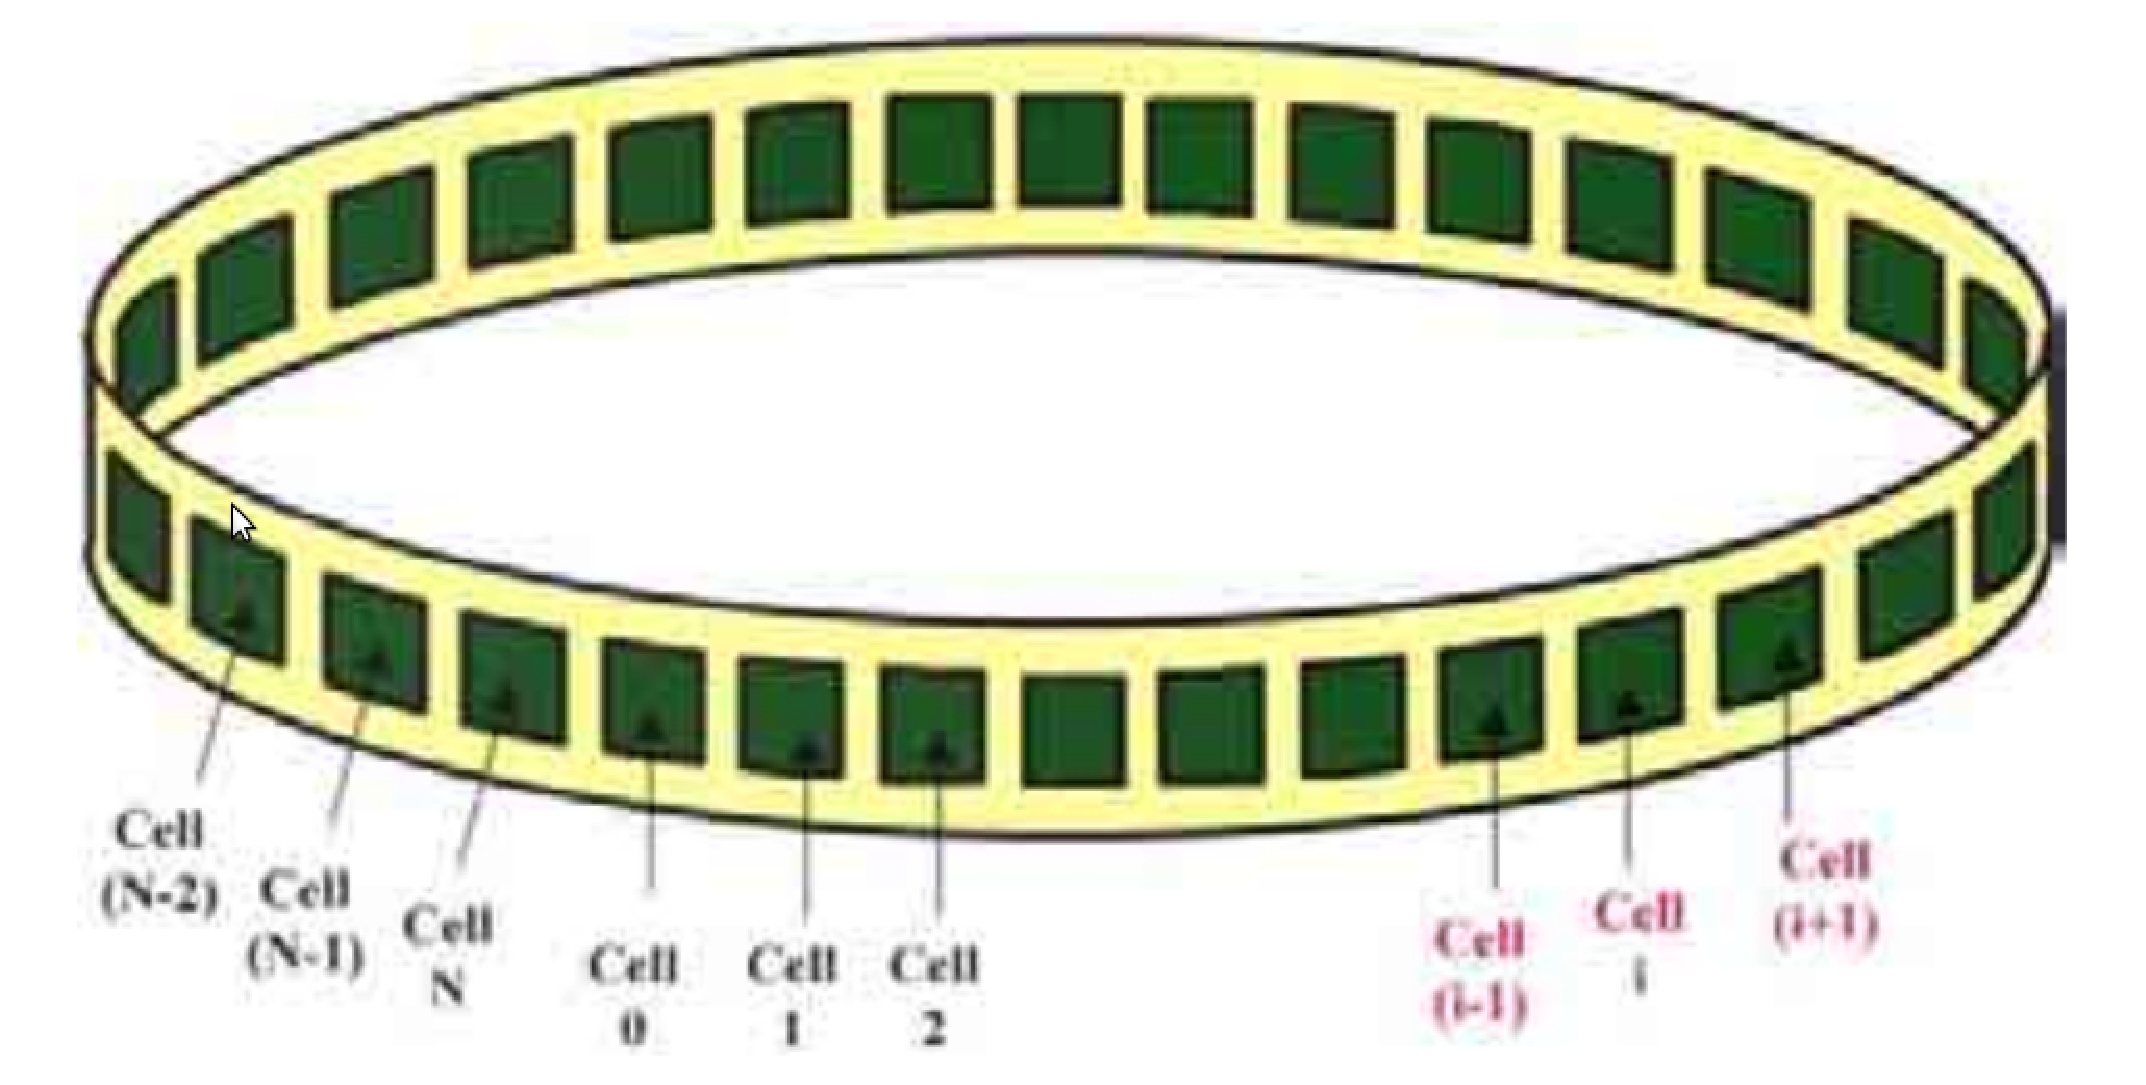
\includegraphics[scale=0.3]{img/ring.eps}
\caption{Condição de contorno periódica: a última célula é ligada à primeira,
formando um anel \citecustom{chua2002a}.}
\label{fig:ring}
\end{center}
\end{figure}

A evolução de um autômato unidimensional pode ser visualizada por meio de uma grade bidimensional
onde cada linha representa uma configuração global em um determinado instante de tempo discreto,
conforme visualizado na Figura \ref{fig:celautomaton}.

\begin{figure}[htp]
\begin{center}
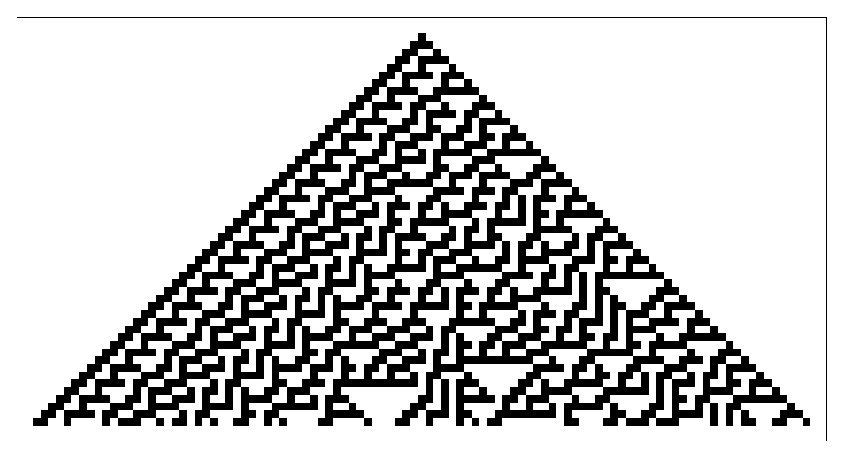
\includegraphics[scale=0.8]{img/CellularAutomaton.eps}
\caption{Evolução temporal de um autômato celular unidimensional.}
\label{fig:celautomaton}
\end{center}
\end{figure}

Existem $2^3=8$ possíveis padrões de estados dentro de uma vizinhança para ACs.
Cada combinação pode resultar nos valores 0 ou 1, assim podem existir $2^{2^3}=256$ ACS
elementares. A regra local pode ser formalizada como:

\begin{equation}
x^{t+1}_i = \phi(x^t_{i-1}, x^t_i, x^t_{i+1})
\end{equation}

Onde $x^t_i$ é o estado da célula $i$ no instante $t$ em que a regra local atua, e $\phi$ é a função
que executa a regra local.  A Tabela \ref{tab:localrule} mostra como é aplicada a regra local.
As regras locais para ACs podem ser descritas por um número número binário de
oito dígitos, codificado pelo resultado das oito combinações de vizinhança da regra local
\citecustom{wolfram1983}. No caso da Figura \ref{fig:celnumbering}, este número é o número $90_{10}$, e
este autômato é chamado de \textit{regra 90}.

\begin{table}[htp]
\begin{center}
\begin{tabular}{|c|c|c|c|}
\hline
\Large $x_{i-1}$ & \Large $x_i$ & \Large $x_{i+1}$ & \Large $\phi$ \\ \hline
1 & 1 & 1 & 0 \\ \hline
1 & 1 & 0 & 1 \\ \hline
1 & 0 & 1 & 0 \\ \hline
1 & 0 & 0 & 1 \\ \hline
0 & 1 & 1 & 1 \\ \hline
0 & 1 & 0 & 0 \\ \hline
0 & 0 & 1 & 1 \\ \hline
0 & 0 & 0 & 0 \\ \hline
\end{tabular}
\caption{Aplicação de regra local.}
\label{tab:localrule}
\end{center}
\end{table}

\begin{figure}[htp]
\begin{center}
\[ \fbox {
{\Large
\begin{tabular}{c c c c c c c c c c c}
$\frac{1 1 1}{0}$ & $\frac{1 1 0}{1}$ & $\frac{1 0 1}{0}$ & $\frac{1 0 0}{1}$ & 
$\frac{0 1 1}{1}$ & $\frac{0 1 0}{0}$ & $\frac{0 0 1}{1}$ & $\frac{0 0 0}{0}$ &
= & 90
\end{tabular}
}
} \]
\caption{Exemplo de esquema de numeração de Wolfram para ACs unidimensionais
\citecustom{wolfram1983}.}
\label{fig:celnumbering}
\end{center}
\end{figure}

\subsection{Equivalência Dinâmica de Regras}

Duas regras locais ${\phi}_1$ e ${\phi}_2$ são ditas equivalentes se e somente se existir
uma transformação a qual mapeia a regra ${\phi}_1$ na regra ${\phi}_2$, e vice-versa
\citecustom{chua2002a}. Estas transformações podem ser de três tipos:

\begin{description}

\item[Transformação de complemento] nesta transformação todos os estados são complementados,
ou seja, troca-se 0 por 1 e vice-versa, conforme exemplificado na Figura \ref{fig:complement}.

\begin{figure}[htp]
\begin{center}
\begin{tabular}{|c|c|c|c|c|c|c|c|c|}
\hline
\Large \textbf{Vizinhança}  & 111 & 110 & 101 & 100 & 011 & 010 & 001 & 000 \\ \hline
\Large \textbf{$\phi$}      &  0  &  1  &  1  &  0  &  1  &  1  &  1  &  0  \\ \hline
\hline
\Large \textbf{Complemento} & 000 & 001 & 010 & 011 & 100 & 101 & 110 & 111 \\ \hline
\Large \textbf{$\phi$}      &  1  &  0  &  0  &  1  &  0  &  0  &  0  &  1  \\ \hline
\hline
\Large \textbf{Reordenado}  & 111 & 110 & 101 & 100 & 011 & 010 & 001 & 000 \\ \hline
\Large \textbf{$\phi$}      &  1  &  0  &  0  &  0  &  1  &  0  &  0  &  1  \\ \hline
\end{tabular}
\caption{Transformação de complemento.}
\label{fig:complement}
\end{center}
\end{figure}

\item[Transformação por reflexão] nesta transformação o estado do vizinho da direita é
trocado com o estado do vizinho da esquerda. A Figura \ref{fig:reflex} ilustra o processo.

\begin{figure}[htp]
\begin{center}
\begin{tabular}{|c|c|c|c|c|c|c|c|c|}
\hline
\Large \textbf{Vizinhança}  & 111 & 110 & 101 & 100 & 011 & 010 & 001 & 000 \\ \hline
\Large \textbf{$\phi$}      &  0  &  1  &  1  &  0  &  1  &  1  &  1  &  0  \\ \hline
\hline
\Large \textbf{Reflexão}    & 111 & 001 & 101 & 011 & 100 & 010 & 110 & 000 \\ \hline
\Large \textbf{$\phi$}      &  0  &  1  &  1  &  0  &  1  &  1  &  1  &  0  \\ \hline
\hline
\Large \textbf{Reordenado}  & 111 & 110 & 101 & 100 & 011 & 010 & 001 & 000 \\ \hline
\Large \textbf{$\phi$}      &  0  &  1  &  1  &  1  &  0  &  1  &  1  &  0  \\ \hline
\end{tabular}
\caption{Transformação do tipo reflexão.}
\label{fig:reflex}
\end{center}
\end{figure}

\newpage

\item[Transformação conjunta] neste caso é realizada uma operação conjunta das duas
operações anteriores.

\end{description}

Para os 256 ACs elementares, existem 88 classes de regras equivalentes.
A Tabela \ref{tab:equiv} lista todas as classes de equivalência. A classe com o menor número
de regra é escolhida como representante de classe.

\begin{table}[H]
\begin{minipage}[b]{0.3\linewidth}\centering
\begin{tabular}{|c|c|}
\hline
\footnotesize Representante & \footnotesize Regras \\
{\footnotesize da classe} & \footnotesize equivalentes \\ \hline
0   & 255 \\ \hline
1   & 127 \\ \hline
2   & 16,191,247 \\ \hline
3   & 17,63,119 \\ \hline
4   & 223 \\ \hline
5   & 95 \\ \hline
6   & 20,159,215 \\ \hline
7   & 21,431,87 \\ \hline
8   & 64,239,253 \\ \hline
9   & 65,111,125 \\ \hline
10  & 80,175,245 \\ \hline
11  & 47,81,117 \\ \hline
12  & 68,207,221 \\ \hline
13  & 69,79,93 \\ \hline
14  & 84,143,213 \\ \hline
15  & 85 \\ \hline
18  & 183 \\ \hline
19  & 55 \\ \hline
22  & 151 \\ \hline
23  & \\ \hline
24  & 66,189,231 \\ \hline
25  & 61,67,103 \\ \hline
26  & 82,167,181 \\ \hline
27  & 39,53,83 \\ \hline
28  & 70,157,199 \\ \hline
29  & 71 \\ \hline
30  & 86,135,149 \\ \hline
32  & 251 \\ \hline
33  & 123 \\ \hline
34  & 48,187,243 \\ \hline
\end{tabular}
\end{minipage}
\hspace{0.3cm}
\begin{minipage}[b]{0.3\linewidth}
\centering
\begin{tabular}{|c|c|}
\hline
\footnotesize Representante & \footnotesize Regras \\
{\footnotesize da classe} & \footnotesize equivalentes \\ \hline
35  & 49,59,115 \\ \hline
36  & 219 \\ \hline
37  & 91 \\ \hline
38  & 52,155,211 \\ \hline
40  & 96,235,249 \\ \hline
41  & 97,107,121 \\ \hline
42  & 112,171,241 \\ \hline
43  & 113 \\ \hline
44  & 100,203,217 \\ \hline
45  & 75,89,101 \\ \hline
46  & 116,139,209 \\ \hline
50  & 179 \\ \hline
51  & \\ \hline
54  & 147 \\ \hline
56  & 98,185,227 \\ \hline
57  & 99 \\ \hline
58  & 114,163,177 \\ \hline
60  & 102,153,195 \\ \hline
62  & 118,131,145 \\ \hline
72  & 237 \\ \hline
73  & 109 \\ \hline
74  & 88,173,229 \\ \hline
76  & 205 \\ \hline
77  & \\ \hline
78  & 92,141,197 \\ \hline
90  & 165 \\ \hline
94  & 133 \\ \hline
104 & 233 \\ \hline
105 & \\ \hline
106 & 120,169,225 \\ \hline
\end{tabular}
\end{minipage}
\hspace{0.3cm}
\begin{minipage}[b]{0.3\linewidth}
\centering
\begin{tabular}{|c|c|}
\hline
\footnotesize Representante & \footnotesize Regras \\
{\footnotesize da classe} & \footnotesize equivalentes \\ \hline
108 & 201 \\ \hline
110 & 124,137,193 \\ \hline
122 & 161 \\ \hline
126 & 129 \\ \hline
128 & 254 \\ \hline
130 & 144,190,246 \\ \hline
132 & 222 \\ \hline
134 & 148,158,214 \\ \hline
136 & 192,238,252 \\ \hline
138 & 174,208,244 \\ \hline
140 & 196,206,220 \\ \hline
142 & 212 \\ \hline
146 & 182 \\ \hline
150 & \\ \hline
152 & 188,194,230 \\ \hline
154 & 166,180,210 \\ \hline
156 & 198 \\ \hline
160 & 250 \\ \hline
162 & 176,186,242 \\ \hline
164 & 218 \\ \hline
168 & 224,234,248 \\ \hline
170 & 240 \\ \hline
172 & 202,216,228 \\ \hline
178 & \\ \hline
184 & 226 \\ \hline
200 & 236 \\ \hline
204 & \\ \hline
232 & \\ \hline
& \\ \hline
& \\ \hline
\end{tabular}
\end{minipage}
\caption{Autômatos celulares elementares equivalentes \citecustom{wolfram1994}.}
\label{tab:equiv}
\end{table}

As Figuras \ref{fig:rule30} e \ref{fig:rule86} mostram a evolução de duas regras locais
equivalentes. Nota-se pelas figuras que a evolução de uma é o espelho da outra.

\begin{figure}[ht]
\begin{minipage}[b]{0.5\linewidth}
\centering
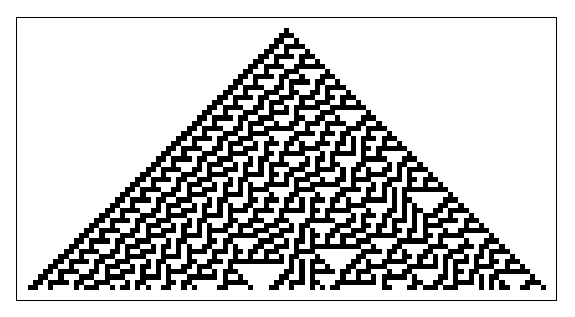
\includegraphics[scale=0.85]{img/rule30.eps}
\caption{Regra 30.}
\label{fig:rule30}
\end{minipage}
\hspace{0.5cm}
\begin{minipage}[b]{0.5\linewidth}
\centering
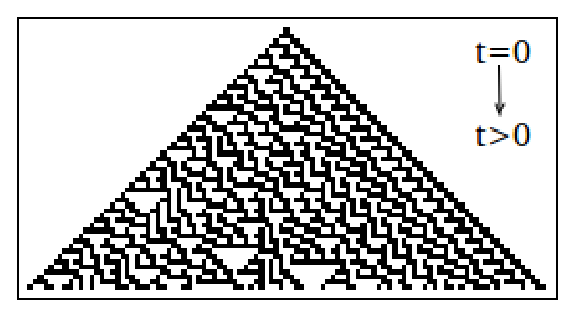
\includegraphics[scale=0.85]{img/rule86.eps}
\caption{Regra 86.}
\label{fig:rule86}
\end{minipage}
\end{figure}

Estudar as classes de equivalência mostra-se importante porque regras locais
equivalentes apresentam o mesmo padrão de complexidade de evolução.

\subsection{Classificação dos Autômatos Celulares}

\citeonline{wolfram1994} dividiu os ACs elementares em quatro
classes segundo a complexidade do padrão gerado pelo seu comportamento dinâmico,
conforme descrito a seguir:

\begin{description}
\item[Classe 1] a evolução leva a um estado homogêneo (ponto fixo).
\item[Classe 2] a evolução leva a um conjunto de estruturas periódicas.
\item[Classe 3] a evolução leva a um padrão caótico.
\item[Classe 4] a evolução leva a estruturas localizadas complexas.
\end{description}

Os atratores nas classes 1, 2 e 3 são respectivamente análogos aos atratores
de ponto fixo, ciclo limite e caóticos encontrados em sistemas dinâmicos
contínuos. A Figura \ref{fig:classes} mostra exemplos de ACs
das quatro classes de complexidade.

\begin{figure}[htp]
\begin{center}
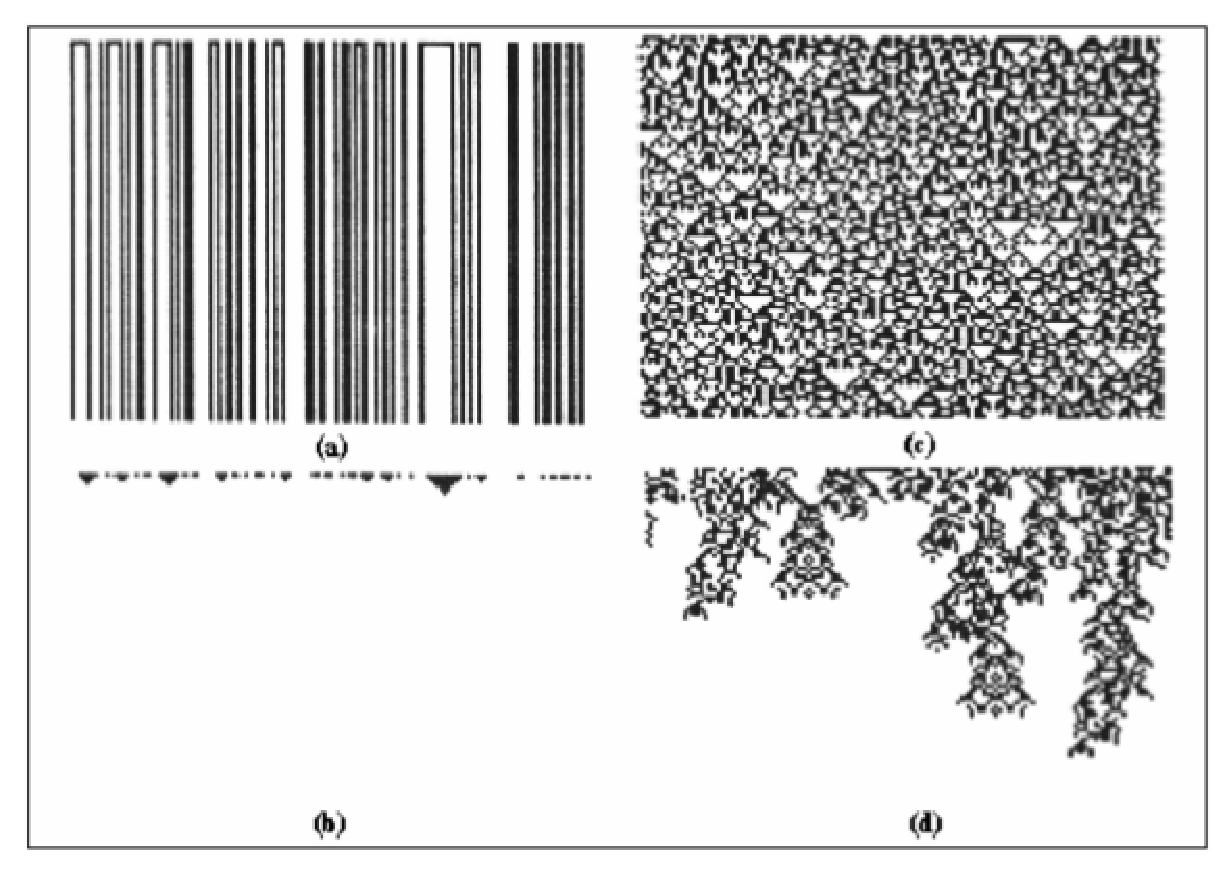
\includegraphics[scale=0.5]{img/classes.eps}
\caption{Classes dinâmicas dos ACs \citecustom{wolfram1984}.
(a) classe 1, (b) classe 2, (c) classe 3 e (d) classe 4.}
\label{fig:classes}
\end{center}
\end{figure}

Trabalhos posteriores se concentraram em formalizar a classificação intuitiva
feita por Wolfram \citecustom{sarkar2000}. \citeonline{culik1988} propuseram a seguinte
classificação.  Seja $\rho$ a regra local para o AC, então:

\begin{enumerate}
\item A regra $\rho$ está na classe 1 se e somente se toda configuração finita,
isto é, configurações nas quais somente um número finito de células estão em
estados não quiescentes, evoluem para uma configuração estável em muitos passos
finitos.

\item A regra $\rho$ está na classe 2 se e somente se toda configuração finita
evolui para uma configuração periódica em um número finito de passos.

\item A regra $\rho$ está na classe 3 se e somente se é decidível se a
configuração ocorre na órbita de outra.

\item A classe 4 engloba todas as regras locais.
\end{enumerate}

\subsection{Linguagens Formais}

A teoria dos autômatos é o estudo dos dispositivos de computação abstratos,
ou \textit{máquinas}. Antes de existirem computadores, na década de 1930, Alan
Turing estudou uma máquina abstrata que tinha todas as características dos
computadores atuais, pelo menos no que se refere ao quanto eles poderiam 
calcular. O objetivo de Turing era descrever com exatidão o limite entre
o que uma máquina de computação podia fazer e aquilo que ela não podia fazer.

Nas décadas de 1940 e 1950, tipos de máquinas mais simples, que hoje são
conhecidas como \textit{autômatos finitos}, foram estudados por diversos
pesquisadores. Esses autômatos, propostos originalmente para modelar a
função do cérebro, se mostraram extremamente úteis para uma grande variedade
de propósitos. Também no final dos anos 50, o linguista N. Chomsky, iniciou
o estudo de gramáticas formais. Embora não sejam estritamente máquinas,
essas gramáticas têm relacionamentos estreitos com os autômatos abstratos
\citecustom{hopcroft2002}.

Linguagens regulares estão entre os tópicos mais antigos em teoria de
linguagens formais. O estudo formal de linguagens regulares
e AFs é datado do início da década de 40, quando máquinas
de estado finito foram utilizadas para modelar conjuntos de neurônios
por McCulloch e Pitts. Desde então, linguagens regulares têm sido
extensivamente estudadas. Resultados das primeiras investigações são,
por exemplo, o teorema de Kleene estabelecendo a equivalência de
expressões regulares e AFs, a introdução de autômatos
com saída por Mealy e Moore, a introdução de AFs não
determinísticos por Rabin e Scott, e a caracterização de linguagens
regulares por congruência de índices finitos por Myhill e Nerode
\citecustom{rozenberg1997}.

O elemento básico de uma linguagem é o alfabeto, um conjunto finito de símbolos
utilizados para formar as palavras pertencentes à linguagem. Por exemplo, o
alfabeto $\Sigma = \{0,1\}$ contém os símbolos $0$ e $1$, e todas as palavras
formadas a partir deste alfabeto só poderão conter estes símbolos.

Uma palavra ou cadeia sobre um alfabeto é uma sequência finita de símbolos
pertencentes a este alfabeto. Assim, $011101$ é uma palavra sobre o alfabeto
$\Sigma = \{0, 1\}$. Uma palavra pode não conter nenhum símbolo. Neste caso,
ela recebe o nome de cadeia \textit{vazia}, e é denotada por $\varepsilon$.
O conjunto de todas as palavras não vazias sobre um alfabeto $\Sigma$ é
denotado por $\Sigma^+$, e o conjunto de todas as palavras, incluindo
a cadeia vazia, sobre um alfabeto $\Sigma$ é denotado por
${\Sigma}^+ \bigcup \varepsilon = \Sigma^*$. O comprimento de uma palavra
é o número de símbolos que a forma. Logo, o comprimento da palavra
\emph{abcd} é 4. Denota-se o comprimento de uma cadeia $w$ por
$|w|$; portanto, $|101| = 3$ e $|\varepsilon| = 0$. Alternativamente,
por meio de um isomorfismo natural, uma cadeia $w \in \Sigma^*$ pode ser
considerada como uma função $w: \{1,\ldots,|w|\} \mapsto \Sigma$; o
valor de $w(j)$, onde $1 \le j \le |w|$ é o símbolo que ocupa a j-ésima
posição em $w$ \citecustom{lewis2008}.

Dá-se o nome de \textbf{linguagem} a qualquer conjunto de palavras sobre um
alfabeto $\Sigma$, ou seja, a qualquer subconjunto de $\Sigma^*$. Portanto,
$\Sigma^*$, $\emptyset$ e $\Sigma$ são linguagens. Sendo uma linguagem 
simplesmente um tipo particular de conjunto, pode-se especificar linguagens
finitas enumerando-se todas as suas palavras. Por exemplo, $\{aba, czr, d, f\}$
é uma linguagem sobre $\{a, b, \ldots, z\}$. Entretanto, a maioria das
linguagens são infinitas, não sendo portanto possível listar todas as palavras
\citecustom{lewis2008}. Assim, especifica-se linguagens infinitas da seguinte forma:

\begin{center}
$L = \{w \in \Sigma^*: \mbox{ w possui a propriedade P}\}$
\end{center}

Nota-se que uma linguagem sobre $\Sigma$ não precisa incluir palavras com todos
os símbolos de $\Sigma$; assim, uma vez que se estabelece que $L$ é uma
linguagem sobre $\Sigma$, também sabe-se que ela é uma linguagem sobre qualquer
alfabeto que seja um superconjunto de $\Sigma$ \citecustom{hopcroft2002}.

\subsection{Autômatos Finitos e Linguagens Regulares}

Segundo \citeonline{hopcroft2002}, um AF é definido por
uma quíntupla $A = (\mathbb{Q},\Sigma,\delta,q_0,\mathbb{F})$, onde:

\begin{description}
\item[$A$] é o nome associado ao AF.
\item[$\mathbb{Q}$] é um conjunto finito de estados.
\item[$\Sigma$] é um conjunto finito de símbolos de entrada
\item[$\delta$] é uma função de transição do tipo $\delta: \mathbb{Q} \times \Sigma \mapsto \mathbb{Q}$.
A função de transição toma um estado e um símbolo de entrada e retorna um novo estado.
$\delta$ também é chamada de \textit{tabela de transição de estados}.
\item[$q_0$] é o estado inicial.
\item[$\mathbb{F}$] é o conjunto de estado finais. $\mathbb{F} \subseteq \mathbb{Q}$.
\end{description}

O autômato atua lendo símbolos de uma fita de entrada onde cada posição na fita
contém um símbolo. O autômato começa seu processamento no estado inicial $q_0$ e,
a cada símbolo lido da fita de entrada, a função de transição
$\delta: \mathbb{Q} \times \Sigma \mapsto \mathbb{Q}$ define um novo estado como o estado atual.
Quando o processamento da fita de entrada termina, se o estado atual for
um dos estados pertencentes ao conjunto $\mathbb{F}$ de estados finais, a entrada é
considerada aceita, caso o contrário, a entrada é rejeitada. Por exemplo,
considere o seguinte AF:

\begin{center}
$M = \{ \mathbb{Q} = \{A,B\}, \break \Sigma = \{0,1\}, \break
\delta = \{A \times 0 \mapsto A; A \times 1 \mapsto B; B \times 0 \mapsto A; B \times 1 \mapsto B\}, \break
q_0 = A, \break \mathbb{F} = \{B\} \}$
\end{center}

Neste caso, o estado inicial é o estado $A$, e o conjunto de estados finais
é formado pelo estado único $B$. É fácil verificar que este autômato aceita
qualquer palavra sobre o alfabeto $\{0,1\}$ que termine com o símbolo $1$.
Considere a cadeia $00101$. O autômato começa no estado $A$ e lê o primeiro
símbolo $0$, a função $\delta$ possui uma entrada $A \times 0 \mapsto A$,
então o autômato consome o símbolo $0$, avança a fita de entrada e permanece
no estado $A$. Novamente um $0$ é lido, então o estado $A$ é mantido e
avança-se a fita de entrada. Agora o símbolo $1$ é lido, a entrada correspondente
na tabela de transição é $A \times 1 \mapsto B$, então o autômato vai para
o estado $B$. O próximo símbolo da entrada é o $0$, e a entrada correspondente
na tabela de transição é $B \times 0 \mapsto A$, então o autômato vai para o
estado $A$. O último símbolo de entrada é o símbolo $1$, então o autômato vai
para o estado $B$. Como toda a entrada foi consumida e o estado atual $B$
pertence ao conjunto de estados finais $\mathbb{F}$, a cadeia de entrada $00101$ é
aceita.

AFs também podem ser representados graficamente através de
um grafo orientado. Os estados são representados pelos nós do grafo
e os arcos representam as transições de estado. O estado inicial possui
uma seta de entrada e os estados finais possui um círculo duplo. A
Figura \ref{fig:automata} mostra graficamente o autômato anterior.

\begin{figure}[htp]
\begin{center}
\begin{VCPicture}{(0,-2)(3,2)}
\State[A]{(0,0)}{A} \FinalState[B]{(3,0)}{B}
\Initial{A} %\Final{B}
\ArcL{A}{B}{1} \ArcL{B}{A}{0}
\LoopN{A}{0} \LoopN{B}{1}
\end{VCPicture}
\caption{Autômato finito representado como um grafo orientado.}
\label{fig:automata}
\end{center}
\end{figure}

O AF anteriormente exemplificado é chamado de AF determinístico.
Em um AF determinístico, cada transição na função de transição possui apenas
um único estado objetivo, ou seja, cada entrada da tabela de transição possui a forma
$\delta: \mathbb{Q} \times \Sigma \mapsto \mathbb{Q}$. Nos AFs não
determinísticos, cada entrada na tabela de transição é da forma
$\delta: \mathbb{Q} \times \Sigma \mapsto 2^{\mathbb{Q}}$,
ou seja, para um dado estado e um símbolo de entrada, o número de possíveis
transições pode ser maior que um \citecustom{rozenberg1997}.  Um autômato não
determinístico também pode possuir mais de um estado inicial.

O processamento em um autômato não determinístico é análogo à sua contraparte
determinística, exceto que quando existe uma ambiguidade na transição (existe
mais de um estado objetivo para uma dada entrada), o autômato se replica, tomando
o caminho dos $n$ estados objetivos. A entrada é considerada aceita se, ao
final do processamento, pelo menos uma instância do autômato está em um
estado final.

O conjunto de palavras reconhecidas por um autômato forma a linguagem do
autômato. Seja $M$ um autômato, $L(M)$ constitui sua linguagem. A classe
de linguagens reconhecidas por AFs são as linguagens regulares.
Linguagens regulares podem também ser representadas por meio das chamadas
expressões regulares. Uma expressão regular é construída a partir dos
seguintes elementos \citecustom{trafaniuc2004}:

\begin{enumerate}
\item O alfabeto de símbolos $\sigma \in \Sigma$;
\item $xy$ representa a concatenação de $x$ e $y$;
\item $x+y$ representa $x$ ou $y$;
\item $x^+$ representa uma ou mais concatenações de $x$;
\item $x^*$ representa qualquer número de concatenações de $x$, incluindo
nenhuma (o que representa a cadeia vazia).
\end{enumerate}

Por exemplo, a expressão regular do autômato da Figura \ref{fig:automata}
é $(0+1)^*1^+$.

\subsection{Evolução de um Autômato Celular}

Linguagens formais consistem do conjunto de palavras formadas a partir de
cadeias de símbolos em um alfabeto finito $\Sigma$ de acordo com regras
gramaticais definidas. Conjuntos de configurações de AFs
podem assim ser considerados como linguagens formais, com cada palavra na
linguagem representando uma configuração do AC. Tais conjuntos
infinitos de configurações são então completamente especificados por
conjuntos finitos de regras gramaticais \citecustom{wolfram1984}.

Os atratores das classes 1 e 2 de AFs elementares podem ser
representados por linguagens regulares simples. Os atratores da classe 3 podem
ser representados por linguagens regulares mais complexas. Os atratores da
classe 4 podem ou não ser representados por uma linguagem regular \citecustom{li1987}.

O conjunto de configurações possíveis em um AF depois de $t$
passos de evolução pode ser representado por um conjunto $\Omega^{(t)}$.

O seguinte exemplo, retirado de \citecustom{wolfram1984}, ilustra o processo de
geração do AF que representa o conjunto de configurações
possíveis $\Omega^{(t)}$ após $t$ iterações.

Considere a construção do conjunto $\Omega^{(1)}$ gerado por um passo de
tempo na evolução do AC elementar com uma regra
local $\phi$ dada por (regra número 76):

\begin{equation}\label{eqn:r76}
111 \mapsto 0, 110 \mapsto 1, 101 \mapsto 0, 100 \mapsto 0, 011 \mapsto 1, 010 \mapsto 1,
001 \mapsto 0, 000 \mapsto 0
\end{equation}

O valor $a_i^{(1)}$ de uma célula na posição $i$ em uma configuração
$A^{(1)} = \phi A^{(0)} \in \Omega^{(1)}$ depende da vizinhança de três
células $\{a_{i-1}^{(0)},a_i^{(0)},a_{i+1}^{(0)}\}$ na configuração precedente
$A^{(0)} \in \Omega^{(0)}$. A célula adjacente de $a_{i+1}^{(1)}$ depende da
vizinhança sobreposta $\{a_i^{(0)},a_{i+1}^{(0)},a_{i+2}^{(0)}\}$. A
dependência de $a_{i+1}^{(0)}$ em $a_i^{(0)}$ associada com esta sobreposição
de duas células nas vizinhanças pode ser representada por um grafo $g$, conforme
ilustra a Figura \ref{fig:A1}. Os nós no grafo representam as sobreposições
$\{a_i^{(0)},a_{i+1}^{(0)}\}$. Este nós são agregados por arcos direcionados
correspondentes a vizinhanças de três células. A regra local do AC
$\phi$ da Equação \ref{eqn:r76} define uma transformação para cada
vizinhança de três células, e assim associa um símbolo com cada arco de $g$.
Cada possível caminho através de $g$ corresponde a uma configuração particular
$A^{(0)}$. O sucessor $A^{(1)}$ de cada configuração inicial é dado pela
sequência de símbolos associada com os arcos no caminho. As sequências de
símbolos obtidas seguindo todos os caminhos possíveis através de $g$ assim
correspondem a todas as possíveis configurações $A^{(1)}$ obtidas depois
de um passo de tempo na evolução do AC \ref{eqn:r76}. O
conjunto completo $\Omega^{(1)}$ pode assim ser representado pelo grafo
$g$. Está claro que nem todas as possíveis sequências de 0s e 1s podem
aparecer nas configurações de $\Omega^{(1)}$. Por exemplo, não existe um
caminho em $g$ que pode incluir a sequência $111$, e assim nenhuma
configuração em $\Omega^{(1)}$ pode conter blocos de células $111$.

\begin{figure}[htp]
\begin{center}
\begin{VCPicture}{(0,-2)(12,8)}
\State[00]{(0,3)}{A} \State[01]{(6,6)}{B}
\State[10]{(6,0)}{C} \State[11]{(12,3)}{D}
\ArcL{A}{B}{001 \mapsto 0} \LoopW{A}{000 \mapsto 0}
\ArcL{B}{D}{001 \mapsto 1} \ArcL{B}{C}{010 \mapsto 1}
\ArcL{C}{B}{101 \mapsto 0} \ArcL{C}{A}{100 \mapsto 0}
\ArcL{D}{C}{110 \mapsto 1} \LoopE{D}{111 \mapsto 0}
\end{VCPicture}
\caption{O grafo de transição de estados $g$ para um AF
não determinístico que gera as configurações obtidas depois de um passo
de tempo na evolução do AC com a regra número 76.
Possíveis sequências de valores de células são representadas por
caminhos possíveis pelo grafo. Os nós no grafo são rotulados por pares
de valores iniciais das células; os arcos então correspondem a triplas
de valores iniciais das células. Cada tripla é mapeada sob a regra 76
para um valor particular da célula. O grafo com arcos rotulados por estas
células correspondem a todas as configurações possíveis obtidas depois
de um passo de tempo \citecustom{wolfram1984}.}
\label{fig:A1}
\end{center}
\end{figure}

O grafo $g$ da Figura \ref{fig:A1} pode ser considerado como uma grafo
de transição de estados para um AC o qual gera a linguagem
formal $\Omega^{(1)}$. Cada nó de $g$ corresponde a um estado do
AF, e cada arco a uma transição no AF, ou
equivalentemente a uma regra  de produção na gramática representada pelo
AF. O conjunto $\Omega^{(1)}$ assim forma uma linguagem
regular.

\subsection{Semi-autômato}

O grafo da Figura \ref{fig:A1} é definido como um semi-autômato.
De acordo com \citeonline{miki2006}, um semi-autômato é um AF
não determinístico, onde todos os estados da máquina são iniciais
e finais e é definido formalmente por uma tripla $\{\mathbb{Q},\Sigma,\delta\}$,
onde:

\begin{description}
\item[$\mathbb{Q}$] representa o conjunto de estados;
\item[$\Sigma$] é o alfabeto de símbolos;
\item[$\delta:\mathbb{Q} \times \Sigma \mapsto 2^\mathbb{Q}$] é a regra de transição, onde
$2^\mathbb{Q}$ é o conjunto potência de $\mathbb{Q}$ e pode ser representado na forma
$\delta(q,a) = \{p_1,p_2,p_3,\ldots,p_n\}$, onde $q$ é o estado atual, $a$
é o símbolo que a máquina lê, e $\{p_1,p_2,p_3,\ldots,p_n\}$ é o
conjunto de possíveis novos estados;
\end{description}

\subsection{Configuração Inicial de um Autômato Celular}

O espaço de configurações iniciais $\Omega^{(0)}$ de um AC
elementar pode ser qualquer combinação de sequências de 0s e 1s
representando os estados iniciais das células. O AF
que representa tal sequência pode ser visualizado na Figura
\ref{fig:initconfigautomaton}, e sua representação em formato de
semi-autômato como implementado no \textit{software Mathematica}
na Figura \ref{fig:initconfigmathematica}.

\begin{figure}[htp]
\begin{center}
\begin{VCPicture}{(0,-2)(3,2)}
\FinalState[A]{(0,0)}{A}
\Initial{A}
\LoopN{A}{0,1}
\end{VCPicture}
\caption{Possíveis configurações iniciais representadas por um AF
determinístico. É fácil perceber que o autômato aceita qualquer sequência de
0s e 1s.}
\label{fig:initconfigautomaton}
\end{center}
\end{figure}

\begin{figure}[htp]
\begin{center}
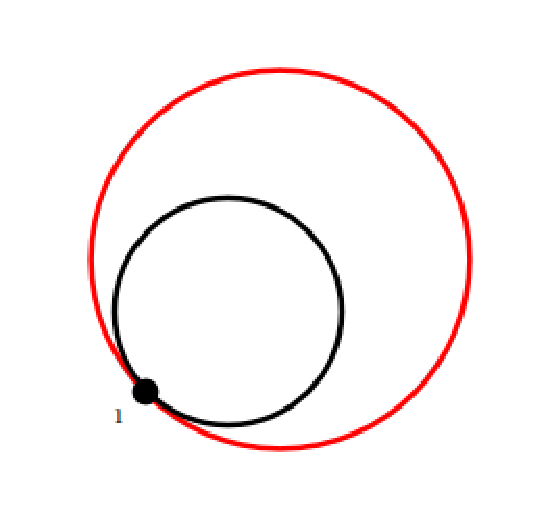
\includegraphics[scale=0.3]{img/InitialConfig.eps}
\caption{Semi-autômato representando as possíveis configurações iniciais
na notação do \textit{software Mathematica}. Arcos vermelhos representam
transições em 0 e arcos pretos representam transições em 1.}
\label{fig:initconfigmathematica}
\end{center}
\end{figure}

Na representação do \textit{Mathematica}, transições em 0 são
representadas por arcos vermelhos e transições em 1 são
representadas por arcos pretos.

\subsection{Funções NetCAStep, TrimNet e MinNet}

\emph{NetCAStep}, \emph{TrimNet} e \emph{MinNet} \citecustom{wolfram2002} são
funções desenvolvidas no \textit{Mathematica} para gerar AFs
que representam a evolução para um passo de tempo de um AC
elementar.

Dado um semi-autômato relacionado à configuração do AC para
um instante de tempo $t$, a função \emph{NetCAStep} \citecustom{wolfram2002}
retorna um AF relacionado ao instante de tempo $t+1$
\citecustom{miki2006}.

A função \emph{NetCAStep} gera como saída uma lista de transições
de estados correspondente a um AF não determinístico.
Sobre a lista de transições de estado resultante da função
\emph{NetCAStep} é aplicada a função \emph{TrimNet}, que, por sua vez,
preserva todos os estados acessíveis por qualquer nó da rede
\citecustom{miki2006}.

É possível encontrar um autômato mínimo que representa um conjunto
de sequências. Isto pode ser feito criando primeiro um autômato
determinístico no qual no máximo um arco de cada valor sai de cada
nó, assim combinando nós equivalentes. Este procedimento é
executado pela função \emph{MinNet} \citecustom{wolfram2002}.

\subsection{Autômatos Celulares como Sistemas Lineares}

\citeonline{wang2011} descreveram a representação linear de sistemas não
lineares com dinâmica local (o que inclui ACs) por meio do produto de
semi-tensor de matrizes.

A representação linear de tais sistemas é essencialmente uma expansão de
espaço, e qualquer sistema lógico multi agente com $n$ agentes e $m$ estados
pode ser traduzido em um sistema linear de dimensão $m^n$ construindo uma
bijeção adequada. Especificamente, o produto de semi-tensor desenvolvido
por Cheng \citecustom{cheng2007} fornece uma ferramenta para a construção de
tal bijeção \citecustom{wang2011}.  

Primeiro descreve-se um sistema multi agente com lógica dinâmica. Seja
$x_i$ o estado do agente $i$, $i=1,2,\ldots,n$, o qual obtém seu valor
a partir do conjunto finito $\chi$. Cada agente atualiza seu estado de acordo
com uma regra local: $f_i: \chi^n \mapsto \chi$ o qual é um operador lógico.
A dinâmica do sistema pode ser descrita como segue \citecustom{wang2011}:

\begin{equation}
\left\{
\begin{array}{l c r}
x_1(t+1) & = & f_1(x_1(t),\ldots,x_n(t)), \\
x_2(t+1) & = & f_2(x_1(t),\ldots,x_n(t)), \\
\vdots & & \\
x_n(t+1) & = & f_n(x_1(t),\ldots,x_n(t)) \\
\end{array} \right.
\label{eqn:dynsys}
\end{equation}

Denota-se $x(t)=(x_1(t),\ldots,x_n(t))$ como o estado do sistema, $\Phi(.)$
como o operador do sistema integrando todas as funções $f_i$. Então o
Sistema \ref{eqn:dynsys} pode ser reescrito como:

\begin{equation}
\label{eqn:sysint}
x(t+1) = \Phi(x(t))
\end{equation}

Suponha que o número de elementos contidos no conjunto $\chi$ seja $m$, isto é,
cada agente possui $m$ diferentes estados, então existirá $m^n$ diferentes
estados do sistema; aqui um estado do sistema significa que cada agente possui
um estado. A partir de \ref{eqn:dynsys} e \ref{eqn:sysint}, sabe-se que o
operador $\Phi(.)$ apenas translada um estado do sistema em outro. Seja
$g: \chi^n \mapsto \{e_i\}^{m^n}_{i=1}$ um mapeamento um para um do conjunto
de estados do sistema para a base padrão $\{e_i\}^{m^n}_{i=1}$, a qual
pode ser representada na forma linear como segue:

\begin{equation}
\label{eqn:linsys}
g(x(t+1)) = Lg(x(t))
\end{equation}

Onde $L$ é uma matriz de dimensão $m^n \times m^n$. Uma vez que $g(x(t))$
e $g(x(t+1))$ são vetores unitários nos quais somente um elemento é igual
a um, toda coluna da matriz $L$ é um vetor de dimensão $m^n$ onde somente um
elemento é igual a um e todos os outros são iguais a zero. Seja a i-ésima
coluna de $L$ denotada por $L_i$. A partir de \ref{eqn:sysint} e do mapeamento
um para um $g$, sabe-se que para o vetor $e_i$ o mapeamento linear $L$ se traduz
no vetor unitário $g(\Phi(g^{-1}(e_i)))$, assim:

\begin{equation}
L_i = g(\Phi(g^{-1}(e_i))), \quad i=1,\ldots,m^n.
\end{equation}

A partir da análise da matriz $L$, sabe-se que a i-ésima coluna de $L$ é um
vetor unitário.

Baseado na expansão espacial, o sistema lógico não linear \ref{eqn:dynsys}
foi convertido na forma da matriz linear \ref{eqn:linsys}. Assim, os autores
investigam as propriedades do Sistema \ref{eqn:dynsys} analizando a estrutura
da matriz $L$ do sistema \ref{eqn:linsys}. Sobretudo, os autores definem e
provam os seguintes teoremas \citecustom{wang2011}:

\begin{enumerate}
\item Para o Sistema \ref{eqn:dynsys}, todo estado possível do sistema será
atingível a partir de qualquer estado inicial se e somente se os autovalores
da matriz $L$ do sistema \ref{eqn:linsys} são
$e^{\frac{2k\pi i}{m^n}},k=0,1,\ldots,m^n-1$, onde $i$ é o número
imaginário tal que $i^2=-1$.

\item Para os Sistemas \ref{eqn:dynsys} e \ref{eqn:linsys}, se
$e^{\frac{2k\pi i}{r}},k=0,1,\ldots,r-1$ são autovalores de $L$, então o
Sistema \ref{eqn:dynsys} terá um ciclo de período $r$. Adicionalmente,
o número de séries $\left\{e^{\frac{2k\pi i}{r}}\right\}^{r-1}_{k=0}$
é o número de ciclos de comprimento $r$.

\item O conjunto limite do Sistema \ref{eqn:dynsys} consiste de somente um
ponto fixo se e somente se os autovalores da matriz $L$ do sistema \ref{eqn:linsys}
tem um elemento igual a $1$ e todos os outros iguais a $0$.
\end{enumerate}

Como exemplo de aplicação, os autores então aplicam esses resultados ao
problema de nilpotência de ACs elementares.

\subsection{Análise da Complexidade de Linguagens Regulares de Autômatos
Finitos Elementares}

\citeonline{mikietal2011} analisaram o padrão de crescimento da complexidade
de linguagens regulares representando as configurações de ACs
elementares.

Sobre as 256 regras elementares foi o aplicado o algoritmo desenvolvido
por \citeonline{trafaniuc2004} ilustrado na Figura \ref{fig:rulesel} para
seleção de regras que apresentam AFs com crescimento de
complexidade a cada passo de tempo.

\begin{figure}[htp]
\begin{center}
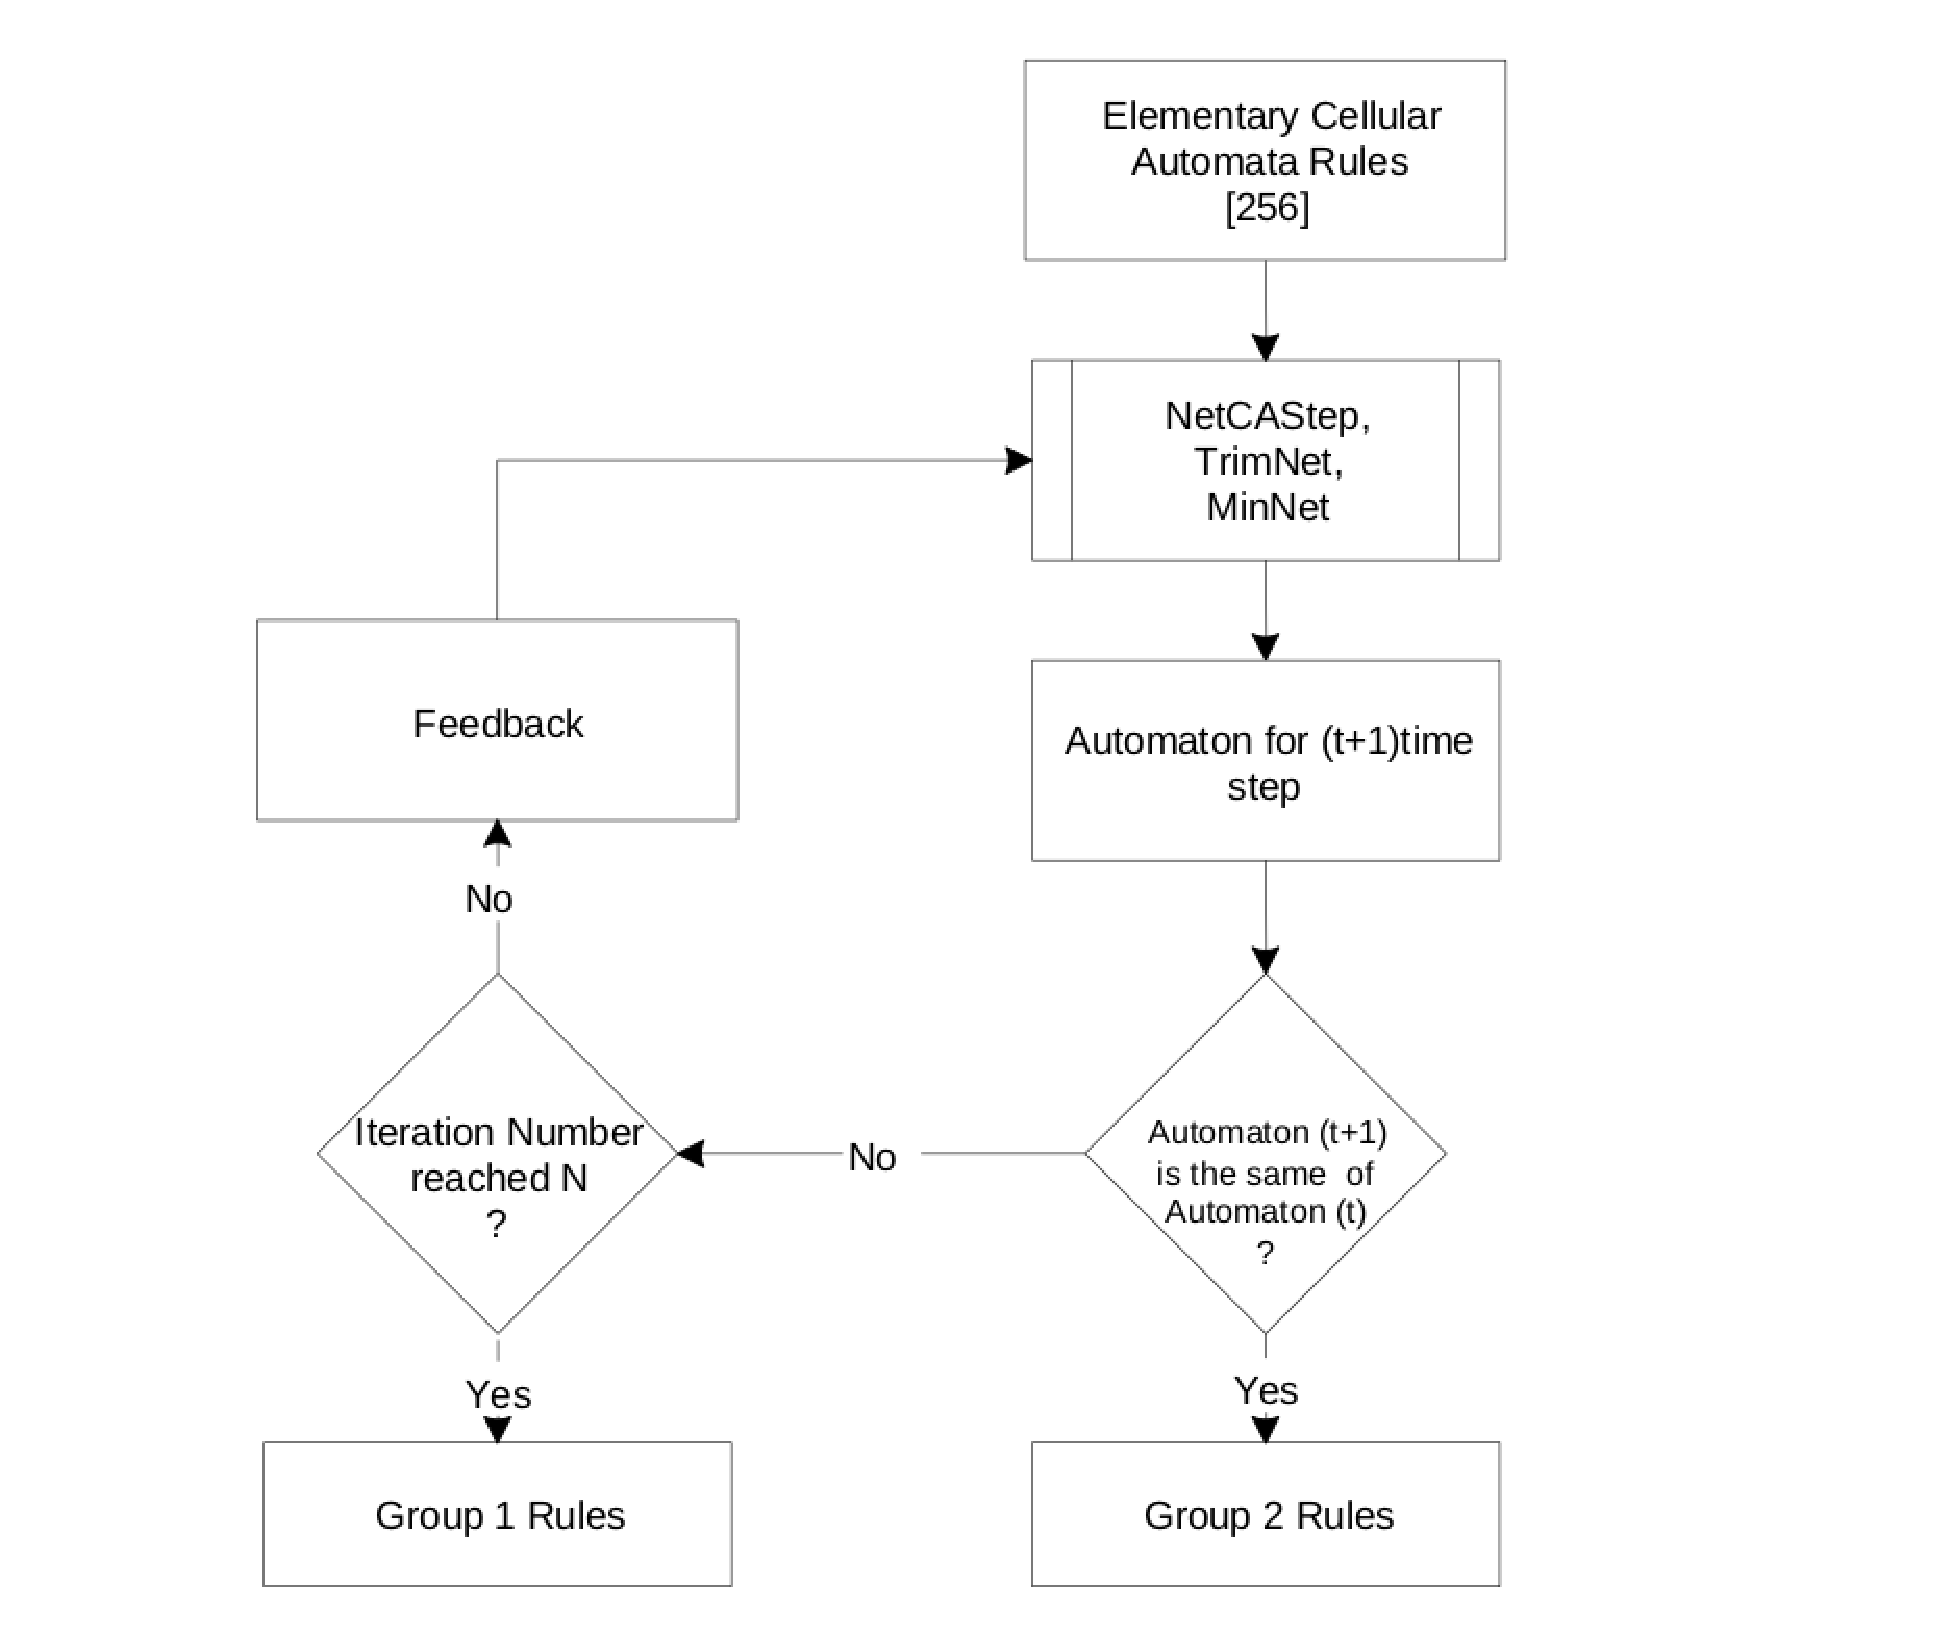
\includegraphics[scale=0.5]{img/rulesel.eps}
\caption{Algoritmo de seleção de regras \citecustom{mikietal2011}.}
\label{fig:rulesel}
\end{center}
\end{figure}

O algoritmo divide as regras em dois grupos \citecustom{mikietal2011}:

\begin{description}
\item[Grupo 1] regras que apresentam crescimento de complexidade no AF
limite a cada passo de tempo, e o método é interrompido quando o
número máximo de passos de execução for atingido.
\item[Grupo 2] regras que deixam de apresentar crescimento de complexidade no
AF em até cinco passos de tempo.
\end{description}

Foram então analisadas as estruturas de crescimento de complexidade das regras
do Grupo 1, primeiro manualmente e, depois, automaticamente por meio do
seguinte método \citecustom{mikietal2011}:

\begin{enumerate}\label{sec:mikialgo}
\item Gerar os grafos das regras de transição, para dois passos de tempo
consecutivos, $t$ e $t+1$, de uma regra do espaço elementar.

\item Gerar todos os possíveis subgrafos do passo de tempo $t+1$ que tenham
o mesmo número de estados que o grafo do passo de tempo $t$.

\item Selecionar todos os subgrafos gerados com base no passo de tempo $t+1$
que se encaixam perfeitamente no grafo do passo de tempo $t$. Ou seja,
selecionar os subgrafos gerados no passo dois, que também são subgrafos do
grafo no tempo $t$.

\item Realizar uma operação de diferença entre o grafo de $t$ e todos os
subgrafos de $t+1$ selecionados no passo três, com o mesmo número de nós. O
subgrafo que apresentar a menor diferença no número de transições de estados
é selecionado. No caso de empate, o primeiro subgrafo é selecionado.
\end{enumerate}

Após a aplicação do método às regras do Grupo 1, foram identificados 26
conjuntos de regras agrupadas em classes de equivalência dinâmicas que
apresentaram estruturas comuns em passos de tempos consecutivos. Todas essas
26 classes foram então analisadas para obtenção de expressões
de crescimento.

O trabalho reconstruiu a tabela de \citecustom{wolfram1994} e acrescentou novas
expressões de crescimento e outros resultados.

\newpage

\section{Construção do Semi-autômato por meio de Matrizes de
Adjacências}\label{sec:desenv}

Conforme já explicado anteriormente, o conjunto de configurações globais de
um AC pode ser descrito por uma linguagem regular e,
consequentemente, por um AF determinístico.

Estudos sobre a complexidade de ACs elementares por meio da
análise dos grafos dos AFs gerados pelas respectivas regras
foram realizados por \citeonline{miki2006} e por \citeonline{trafaniuc2004}.

\citeonline{trafaniuc2004} analisou manualmente as regras do Grupo 1 descrito
na Seção \ref{sec:mikialgo} e encontrou 26 regras que apresentaram padrão
de crescimento do AF gerado para os sucessivos passos de tempo na evolução
do AC. O trabalho deduziu a expressão de crescimento da regra 184, inclusive
um método para obtenção do AF de tempo $t$. Após, o trabalho fez as mesmas
análises para as outras 25 regras. Do total das 26 regras, 16 regras
apresentaram relações entre passos de tempo distintos, sendo elas: 43, 113,
128, 132, 136 140, 142, 162, 168, 176, 184, 192, 196, 212, 224 e 232. Destas
16 regras, para 12 delas foram encontradas as expressões que caracterizam o
crescimento dos semi-autômatos de acordo com o passo de tempo, sendo
apresentado o método de obtenção do semi-autômato de passo $t$ para cada uma.
O trabalho chegou à conclusão que são necessárias duas
propriedades para caracterização do semi-autômato de uma regra
\citecustom{trafaniuc2004}:

\begin{enumerate}
\item O crescimento do número de estados do semi-autômato deve ser
proporcional ao passo de tempo, ou seja, o número de estados cresce
a cada passo de tempo.

\item Os semi-autômatos para passos de tempo distintos devem possuir uma
relação de crescimento, conforme descrito na Seção \ref{sec:mikialgo}.
\end{enumerate}

\citeonline{miki2006} automatizou o processo manual de análise de crescimento
de AFs desenvolvido por \citeonline{trafaniuc2004} por meio de uma operação
de diferença de grafos. O algoritmo foi descrito na Seção
\ref{sec:mikialgo}. Com os resultados, o trabalho passou a focar na análise
da regra 184 no objetivo de obter o autômato limite. O autômato limite
foi construído manualmente como referência, conforme mostrado na Figura
\ref{fig:limit184}.

\begin{figure}[htp]
\begin{center}
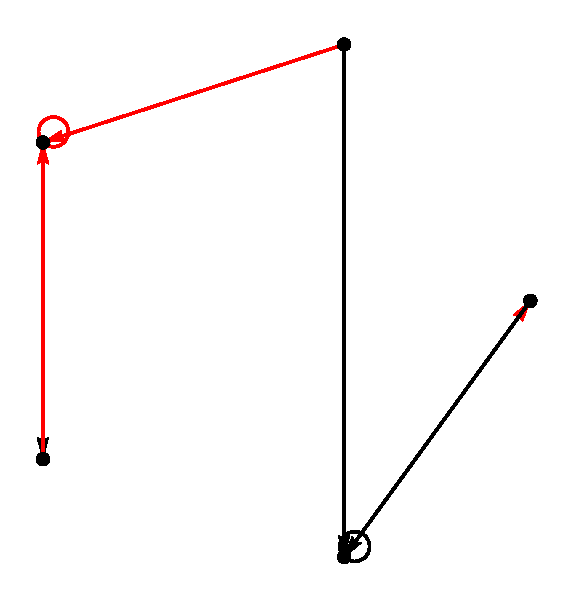
\includegraphics[scale=0.8]{img/limit184.eps}
\caption{Grafo limite da regra 184 \citecustom{miki2006}.}
\label{fig:limit184}
\end{center}
\end{figure}

\citeonline{miki2006} identificou que os semi-autômatos dos sucessivos passos de
tempo da regra são assimétricos, mas o semi-autômato limite é simétrico, e não
conseguiu achar uma operação que faça essa transformação de simetria;
não conseguindo, assim, encontrar o semi-autômato limite da regra 184
partindo-se dos semi-autômatos intermediários.

Neste capítulo, é proposta uma nova abordagem para o problema, por meio da
análise das matrizes de adjacências correspondentes aos AFs
das respectivas regras do espaço elementar. Porém, como será visto adiante,
não é possível representar completamente um AF utilizando a
notação clássica de matrizes de adjacências. É proposta, então, uma
nova notação que, dada a matriz de adjacência, é possível construir
integralmente o grafo da respectiva matriz.

O texto então deduz o algoritmo de formação do AF
de tempo $t$ para a regra 184; e então finaliza com uma breve
descrição dos padrões de formação de matrizes das mesmas regras
estudadas em \citecustom{mikietal2011}. O motivo de escolher
a regra 184 para ilustrar o processo se deve ao fato de ser
uma regra que já foi extensivamente estudada em \citecustom{trafaniuc2004}
e \citecustom{miki2006}.

\subsection{Representação de Semi-autômatos em Forma Matricial}

\subsubsection{Matrizes de Adjacências}

Uma \textit{matriz de adjacências}, algumas vezes também chamada de 
\textit{matriz de conexões}, representa os estados e transições de grafos
em forma matricial, rotulando as linhas e colunas com os vértices do grafo.
As linhas e colunas representam, respectivamente, os estados de origem e destino
do grafo\footnote{No caso de grafos não direcionados, não existe
distinção de estados origem e destino, mas somente grafos direcionados são 
de interesse neste trabalho}.

A representação de um grafo direcionado $G$ com $n$ vértices se dá por uma
matriz $M$ de dimensão $n \times n$. O valor da posição $a_{ij}$ da matriz
$M$ será $1$ se existir uma transição do estado $i$ para o estado $j$.
A Figura \ref{fig:graph} mostra um grafo direcionado e a Figura \ref{fig:adjm}
mostra a matriz de adjacências correspondente.

\begin{figure}[ht]
\begin{minipage}[b]{0.5\linewidth}
\begin{center}
\begin{VCPicture}{(0,-4)(4,1)}
\State[1]{(0,0)}{A} \State[2]{(4,0)}{B}
\State[3]{(2,-2)}{C}
\ArcL{A}{B}{} \ArcR{A}{C}{} 
\ArcL{B}{A}{}
\ArcR{C}{B}{} \LoopS{C}{}
\end{VCPicture}
\caption{Grafo direcionado.}
\label{fig:graph}
\end{center}
\end{minipage}
\hspace{0.5cm}
\begin{minipage}[b]{0.5\linewidth}
\begin{center}
\begin{math}
\begin{pmatrix}
0 & 1 & 1 \\
1 & 0 & 0 \\
0 & 1 & 1
\end{pmatrix}
\end{math}
\caption{Representação em matriz de adjacências.}
\label{fig:adjm}
\end{center}
\end{minipage}
\end{figure}

Embora matrizes de adjacências possam representar grafos direcionados simples,
não é possível representar completamente um semi-autômato, dado que:

\begin{enumerate}
\item É possível haver mais de uma transição do estado $i$ para o estado
$j$, $\exists i,j$.

\item Nos índices da matriz não está codificado o valor da transição, que
é o valor esperado na fita de entrada. Observe que a solução de criar
um mapeamento $f: L \mapsto a_{ij}$ que associa o valor do arco ao índice
da matriz é inviável devido à possibilidade de existir mais de uma
transição por par de estados $(i,j)$.
\end{enumerate}

Para ilustrar a dificuldade de se representar semi-autômatos utilizando
matrizes de adjacências, considere o semi-autômato da Figura
\ref{fig:initconfigautomaton}. A matriz de adjacências deste autômato
seria uma matriz $1 \times 1$ com valor $a_{1,1}=1$. Porém, perde-se a informação
de que existem duas transições reflexivas no semi-autômato. Mais ainda,
não existe qualquer menção ao valor das transições.

Uma notação possível seria utilizar uma lista em cada índice da matriz de
adjacências. Neste caso, o índice $a_{ij}$ conteria uma lista com todos
os possíveis valores de transição do estado $i$ para o estado $j$.
Porém, com este tipo de notação, além de ser mais complicado
detectar padrões nos sucessivos passos de tempo, perde-se qualquer possibilidade
de operações algébricas com as matrizes. Por exemplo, não seria possível
estudar possíveis padrões baseado nos autovalores das matrizes.

A próxima seção introduz uma notação alternativa de matrizes de
adjacências que contorna as dificuldades apresentadas.

\subsubsection{Matrizes de Adjacências Isomórficas}

Uma matriz de adjacências isomórfica é uma notação de matriz de
adjacências para representar semi-autômatos que possui uma relação
de isomorfismo entre a matriz e sua representação em grafo.
Formalmente, dado o conjunto de matrizes de adjacências
isomórficas $\mathbb{M}$ e o conjunto de semi-autômatos $\mathbb{G}$,
existe uma transformação $T: \mathbb{G} \mapsto \mathbb{M}$ e uma
transformação $T^{-1}: \mathbb{M} \mapsto \mathbb{G}$. 

O elemento chave para conseguir essa relação de isomorfismo
é encontrar uma representação do conjunto de transições e
seus respectivos valores em um número real que possa ser codificado
nos índices da matriz, e que possa ser decodificado quando for
aplicada à transformação $T^{-1}$. Formalmente, dado o conjunto de transições
$\mathbb{L}$ do estado $i$ para o estado $j$, $\forall i,j$, encontrar uma
relação $\eta:\mathbb{L} \mapsto \Re$ que seja bijetora.

A resposta para esta questão está em criar um mapeamento dos valores
possíveis de transições para o conjunto de números naturais
$\mathbb{L} \mapsto \mathbb{N}$ e então codificar os valores das transições
em um número binário. Cada bit do número binário corresponde a um valor de
transição. Se o valor no $k$-ésimo bit for 1, significa que existe uma
transição (mapeada no conjunto dos naturais) de valor $k$ do estado de
origem para o estado destino em questão. A operação $\eta$ de codificação dos
arcos $\mathbb{L}$ em um número real é o polinômio de base 2:

\begin{equation}
\eta(\mathbb{L}_{ij}) = \sum_{\forall k \in (\mathbb{L}_{ij} \mapsto \mathbb{N})} 2^k
\end{equation}

Onde $\mathbb{L}_{ij}$ é o conjunto de transições do estado $i$ para o estado
$j$. Repare que como $k \in \mathbb{N}$, então $\eta(\mathbb{L}_{ij}) \in \mathbb{Z}$,
ou seja, $\eta(\mathbb{L}_{ij})$ está restrita ao domínio dos inteiros. Se
$k \in \mathbb{Z}$ ($\mathbb{L}_{ij} \mapsto \mathbb{Z}$), então
$\eta(\mathbb{L}_{ij}) \in \Re$, pois admitiria-se a possibilidade de expoentes negativos.
Como computacionalmente é mais custoso trabalhar-se com números reais do que com inteiros,
e não há benefício aparente em expandir $\eta$ para o domínio dos reais,
já que $\mathbb{N}$ é contavelmente infinito \citecustom{lewis2008}, optou-se
por restringir-se $\eta$ ao domínio dos números inteiros. Outra observação
é a de que a base númerica não necessarimente deve ser base 2. Poderia-se trabalhar com outras
bases. Todavia, a única implicação na mudança de base é a quantidade de dígitos
necessária para representar um dado conjunto $2^{\mathbb{L}}$ de possíveis combinações de
transições e, do ponto de vista de arquitetura computacional, a base 2 é a
base mais natural para se trabalhar. A Figura \ref{fig:semigraph}
mostra o grafo da Figura \ref{fig:graph}, agora representado como um semi-autômato
(repare que agora existe um valor para cada transição), e a Figura \ref{fig:iadjm}
mostra a matriz de adjacências isomórfica correspondente.

\begin{figure}[ht]
\begin{minipage}[b]{0.5\linewidth}
\begin{center}
\begin{VCPicture}{(0,-4)(4,1)}
\State[1]{(0,0)}{A} \State[2]{(4,0)}{B}
\State[3]{(2,-2)}{C}
\ArcL{A}{B}{0} \ArcR{A}{C}{0} 
\ArcL{B}{A}{1}
\ArcR{C}{B}{1} \LoopS{C}{0}
\end{VCPicture}
\caption{Semi-autômato representado através de um grafo direcionado.}
\label{fig:semigraph}
\end{center}
\end{minipage}
\hspace{0.5cm}
\begin{minipage}[b]{0.5\linewidth}
\begin{center}
\begin{math}
\begin{pmatrix}
0 & 1 & 1 \\
2 & 0 & 0 \\
0 & 2 & 1
\end{pmatrix}
\end{math}
\caption{Representação em matriz de adjacências isomórfica.}
\label{fig:iadjm}
\end{center}
\end{minipage}
\end{figure}

A transformação de um semi-autômato em uma matriz de adjacências
isomórfica é executada por meio do Algoritmo \ref{alg:stom}.

\begin{algorithm}
\caption{Algoritmo para gerar a matriz de adjacências isomórfica a partir
de um semi-autômato.}
\label{alg:stom}
\begin{algorithmic}
\STATE $n \leftarrow \mbox{Length}(\mathbb{Q})$ \COMMENT{número de estados}
\STATE $A \leftarrow \mbox{ Matriz nula } n \times n$
\FORALL{$i,j \in \mathbb{Q}$}
\IF{$\mathbb{L}_{ij} \neq \emptyset$}
\STATE $A_{ij} = \eta(\mathbb{\mathbb{L}}_{ij})$
\ENDIF
\ENDFOR
\end{algorithmic}
\end{algorithm}

O algoritmo atua criando uma matriz $A_{n \times n}$, onde $n$ é o número
de estados do semi-autômato, e atribuindo à posição $A_{ij}$ o valor
da função $\eta(\mathbb{L}_{ij}),\forall i,j$, onde $\mathbb{L}_{ij}$
é o conjunto de transições de $i$ para $j$.

O algoritmo de transformação de uma matriz de adjacências isomórfica em
um semi-autômato é baseado na representação binária dos valores dos
índices da matriz. Por exemplo, se no índice $A_{1,2}$ existir o valor
$3$, então existe uma transição em $0$ e uma transição em $1$ do estado
\emph{1} para o estado \emph{2}, pois $2^0+2^1=3$. O Algoritmo \ref{alg:mtos}
mostra o processo de geração do semi-autômato a partir de uma matriz de
adjacências isomórfica. O algoritmo pressupõe a existência de uma função
\emph{MakeTransition(i,j,m)} que cria uma transição em \emph{m} do estado
\emph{i} para o estado \emph{j}.

\begin{algorithm}
\caption{Algoritmo para gerar o semi-autômato a partir de uma matriz de
adjacências isomórfica.}
\label{alg:mtos}
\begin{algorithmic}
\FOR{$i=1$ to $n$}
\FOR{$j=1$ to $n$}
\IF{$A_{ij} \neq 0$}
\REPEAT
\STATE $q = \lfloor A_{ij} \div 2 \rfloor$
\STATE $r = A_{ij}-2q$ \COMMENT{resto}
\IF{$r \neq 0$}
\STATE $n=0$
\WHILE{$2^n \le A_{ij}$}
\STATE $n=n+1$
\ENDWHILE
\STATE MakeTransition$(i,j,n-1)$
\ENDIF
\UNTIL{$q \neq 0$}
\ENDIF
\ENDFOR
\ENDFOR
\end{algorithmic}
\end{algorithm}

O algoritmo executa em tempo $O(n^2)$ em relação à dimensão da matriz.
De posse do Algoritmo \ref{alg:mtos}, é possível criar o algoritmo para gerar o
autômato limite de uma regra apenas elaborando-se um outro algoritmo para gerar a
matriz de adjacências isomórfica da regra. A próxima seção apresenta este
algoritmo para a regra 184.

\subsection{Algoritmo do Semi-autômato de Tempo \emph{t} para a regra 184}\label{sec:184}

Esta seção mostra como utilizar a notação de matriz de adjacências
isomórfica para deduzir um algoritmo que gere o semi-autômato de uma
regra do espaço elementar para um passo de tempo discreto $t$ qualquer. Em
particular, aqui é deduzido o algoritmo para gerar a matriz isomórfica para
a regra 184 e, a partir desta, poderá ser aplicado o Algoritmo \ref{alg:mtos}
para obtenção do semi-autômato.

\citeonline{miki2006}, baseado nos resultados de \citeonline{trafaniuc2004},
estudou extensivamente o padrão de crescimento da regra 184 através da análise
dos semi-autômatos gerados pelos sucessivos passos de tempo. No caso, ele estudou
os semi-autômatos gerados dentro dos cinco primeiros passos de tempo. A Figura
\ref{fig:184-5t} mostra os semi-autômatos da regra 184 gerados para os cinco
primeiros passos de tempo. A notação de grafo é a mesma da Figura
\ref{fig:initconfigmathematica}.

\begin{figure}[htp]
\begin{center}
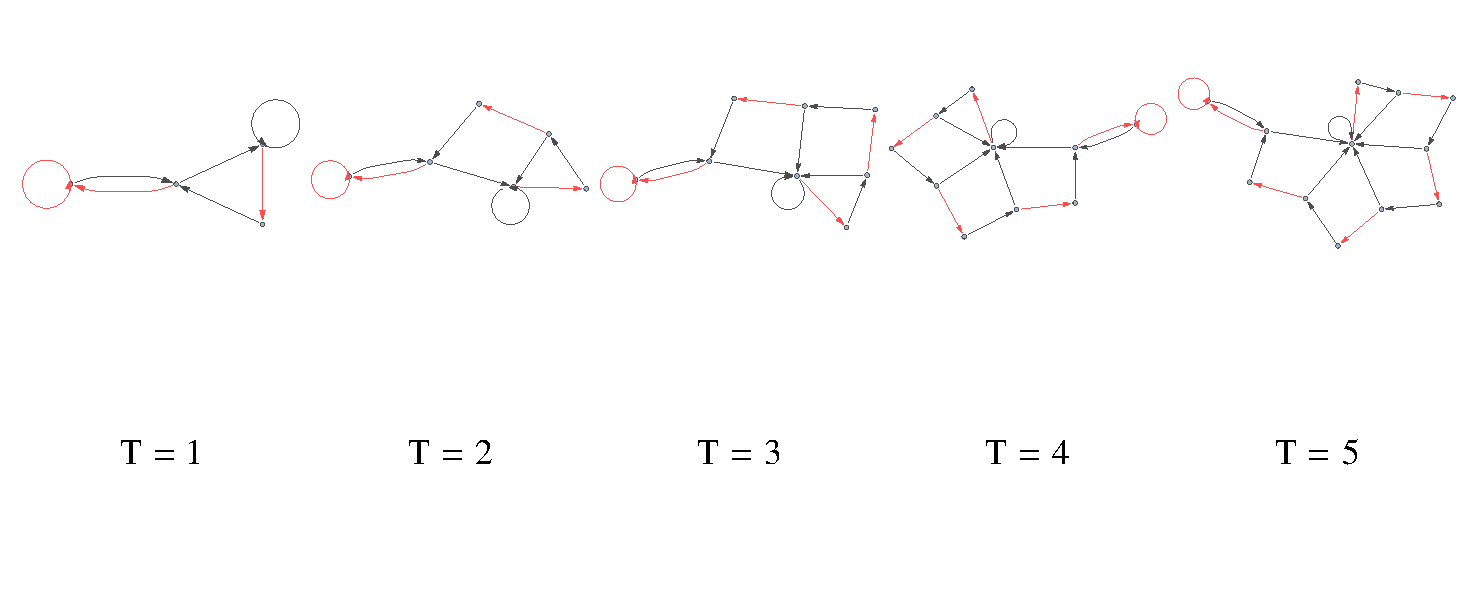
\includegraphics[scale=1]{img/184_5t.eps}
\caption{Semi-autômatos para os cinco primeiros passos de tempo da regra 184.}
\label{fig:184-5t}
\end{center}
\end{figure}

Utilizando o método apresentado na Seção \ref{sec:mikialgo}, sua conclusão
foi a de que a cada passo de tempo, sempre existia uma mesma estrutura
de grafo sendo adicionada e uma sendo excluída, e essas estruturas eram
invariantes no tempo. As Figuras \ref{fig:addstruct} e \ref{fig:excstruct}
mostram, respectivamente, as estruturas adicionada e excluída dos sucessivos
semi-autômatos da regra 184.

\begin{figure}[htp]
\begin{minipage}[b]{0.5\linewidth}
\centering
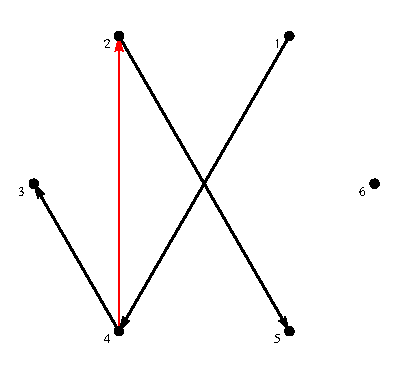
\includegraphics[scale=1]{img/addStruct.eps}
\caption{Estrutura adicionada \citecustom{miki2006}.}
\label{fig:addstruct}
\end{minipage}
\hspace{0.5cm}
\begin{minipage}[b]{0.5\linewidth}
\centering
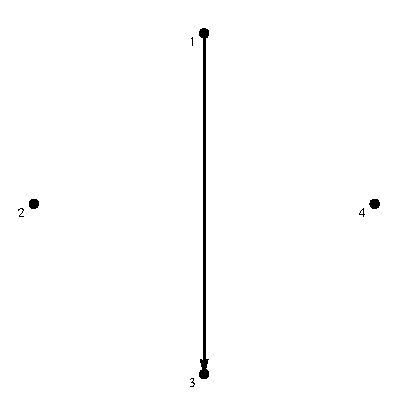
\includegraphics[scale=1]{img/excStruct.eps}
\caption{Estrutura excluída \citecustom{miki2006}.}
\label{fig:excstruct}
\end{minipage}
\end{figure}

É difícil identificar visualmente estas estruturas, ou qualquer padrão de
crescimento, por meio dos semi-autômatos. Porém, convertendo estes grafos
em matrizes de adjacências isomórficas, é possível detectar os padrões
de crescimento e visualizar o efeito das estruturas adicionada e
excluída. As Figuras \ref{fig:addstructm} e \ref{fig:excstructm} mostram
as respectivas estruturas adicionada e excluída em notação matricial, e
a Tabela \ref{tab:mr184} mostra a evolução no tempo da regra 184 em notação
de grafo e matricial.

\begin{figure}[htp]
\begin{minipage}[b]{0.5\linewidth}
\begin{center}
\begin{math}
\begin{pmatrix}
0 & 0 & 0 & 2 & 0 & 0 \\
0 & 0 & 0 & 0 & 2 & 0 \\
0 & 0 & 0 & 0 & 0 & 0 \\
0 & 1 & 2 & 0 & 0 & 0 \\
0 & 0 & 0 & 0 & 0 & 0 \\
0 & 0 & 0 & 0 & 0 & 0
\end{pmatrix}
\end{math}
\caption{Estrutura adicionada em notação matricial.}
\label{fig:addstructm}
\end{center}
\end{minipage}
\hspace{0.5cm}
\begin{minipage}[b]{0.5\linewidth}
\begin{center}
\begin{math}
\begin{pmatrix}
0 & 0 & 2 & 0 \\
0 & 0 & 0 & 0 \\
0 & 0 & 0 & 0 \\
0 & 0 & 0 & 0
\end{pmatrix}
\end{math}
\caption{Estrutura excluída em notação matricial.}
\label{fig:excstructm}
\end{center}
\end{minipage}
\end{figure}

Embora devido à diferença nos tamanhos das matrizes não seja possível
derivar uma operação algébrica, é fácil notar o que acontece na evolução
da regra 184 olhando as matrizes de adjacências da regra e as estruturas
adicionada e excluída.

Observando duas matrizes de tempo $t$ e tempo $t+1$, repara-se que:

\begin{enumerate}
\item Existe uma diagonal de transições em $1$ que começa em $A_{t+1,1}$
e vai até $A_{2t,t}$. A cada passo de tempo, uma transição em $1$ é adicionada,
o que corresponde ao valor $1$ na posição $(4,2)$ da estrutura adicionada.

\item Existe uma coluna de transições em $2$ iniciando-se na posição
$A_{t+1,t+1}$ e terminando na posição $A_{n-1,t+1}$. Novamente observa-se
que a cada passo de tempo, uma linha com uma transição em $2$ é adicionada à
coluna, e essa transição corresponde ao valor $2$ na posição $(4,3)$ na matriz da
estrutura adicionada.

\item Uma diagonal de transições em $2$ aparece na posição $A_{1,t+2}$ indo
até a posição $A_{t,n-1}$. Olhando para a matriz da estrutura adicionada,
observa-se que duas transições em $2$ são adicionadas a esta diagonal a cada
passo de tempo, mas uma dessas transições é retirada conforme se nota na
matriz da estrutura excluída.

\item Por fim, uma transição em $1$ é atribuída à posição $A_{n,n}$, uma
outra transição em $1$ na posição $A_{n-1,n}$ e uma transição em $2$ é
atribuída na posição $A_{n,n-1}$.
\end{enumerate}

Baseando-se nesta análise, é possível derivar um algoritmo de construção da
matriz de adjacências isomórfica do semi-autômato de tempo $t$ para a
regra 184. O algoritmo é mostrado no Algoritmo \ref{alg:r184}.

\begin{algorithm}
\caption{Algoritmo para gerar a matriz de adjacências isomórfica do
semi-autômato de tempo $t$ para a regra 184.}
\label{alg:r184}
\begin{algorithmic}
\STATE $A \leftarrow \mbox{ matriz nula } n \times n \mbox{, onde } n=2(t+1)$
\STATE $i \leftarrow t+1$
\FOR{$j=1$ to t}
\STATE $A_{ij} \leftarrow 1$
\STATE $i \leftarrow i+1$
\ENDFOR
\FOR{$i=t+1$ to $n$}
\STATE $A_{i,t+1} \leftarrow 2$
\ENDFOR
\STATE $j \leftarrow t+2$
\FOR{$i=1$ to $t$}
\STATE $A_{ij} \leftarrow 2$
\STATE $j \leftarrow j+1$
\ENDFOR
\STATE $A_{n,n} \leftarrow 1$
\STATE $A_{n-1,n} \leftarrow 1$
\STATE $A_{n,n-1} \leftarrow 2$
\end{algorithmic}
\end{algorithm}

O algoritmo executa em tempo $O(t)$. A combinação dos Algoritmos
\ref{alg:mtos} e \ref{alg:r184} executa em tempo:

\begin{equation}
\begin{tabular}{ r c l }
\(T\) & \(=\) & \(O(t) + O((2t+2)^2)\) \\
  & \(=\) & \(O(t) + O(4t^2+8t+4)\) \\
  & \(=\) & \(O(t) + O(t^2) + O(t) + O(1)\) \\
  & \(=\) & \(O(t^2)\)
\end{tabular}
\end{equation}

De posse do Algoritmo \ref{alg:r184} e do Algoritmo \ref{alg:mtos} é
possível, então, recriar o semi-autômato de tempo $t$ para a regra 184.

\subsection{Padrão de Formação das Matrizes de Adjacências Isomórficas}\label{sec:pattern}

Após um estudo aprofundado e dedução do algoritmo de formação das matrizes
de adjacências isomórficas para a regra 184 descrito na Seção \ref{sec:184},
estudou-se o padrão de formação para todas as mesmas 26 regras estudadas em
\citecustom{mikietal2011}. Conforme mostrado na Tabela \ref{tab:pattern},
todas as regras apresentam um padrão de formação, embora nem sempre a
partir do primeiro instante de tempo.

\begin{table}[htp]
\begin{center}
\begin{tabular}{c c c}
\hline
\textbf{Regra} & \textbf{Início do padrão de formação} & \textbf{Intercalado}\\ \hline
 11 & $t=4$ & Sim \\
 14 & $t=2$ & Sim \\
 35 & $t=2$ & Sim \\
 43 & $t=1$ & Não \\
 50 & $t=4$ & Sim \\
 56 & $t=2$ & Não \\
 70 & $t=3$ & Não \\
 81 & $t=3$ & Sim \\
 98 & $t=2$ & Não \\
113 & $t=2$ & Não \\
128 & $t=1$ & Não \\
132 & $t=2$ & Não \\
136 & $t=2$ & Não \\
140 & $t=2$ & Não \\
142 & $t=2$ & Não \\
162 & $t=1$ & Não \\
168 & $t=1$ & Não \\
172 & $t=2$ & Não \\
176 & $t=2$ & Não \\
184 & $t=1$ & Não \\
192 & $t=2$ & Não \\
196 & $t=1$ & Não \\
212 & $t=1$ & Não \\
224 & $t=2$ & Não \\
252 & $t=2$ & Não \\
\end{tabular}
\caption{Padrão de formação de matrizes de adjacências isomórficas das
regras elementares.}
\label{tab:pattern}
\end{center}
\end{table}

Além de especificar a regra, a tabela mostra em que passo de tempo a regra
começou a apresentar um padrão de formação e se esse padrão é intercalado
ou não. Por \textit{padrão de formação} entende-se por uma estrutura
presente em $t$ que pode ser vista em $t+1$ de forma expandida ou contraída.
Um \textit{padrão de formação intercalado} significa que existe uma
expansão de um padrão na matriz ocorre a cada dois instantes de tempo.

A partir da Tabela \ref{tab:pattern}, conclui-se que as regras estão divididas
em dois grupos base: as que apresentam um padrão a partir de $t=n$ e as que
apresentam um padrão intercalado a partir de $t=n,\exists n \in \mathbb{N}$.
A análise baseou-se a partir da observação dos cinco primeiros passos de
tempo e, quando o padrão de formação se deu a partir de $t=4$, analisou-se
os dez primeiros passos de tempo. O Apêndice \ref{sec:matrices} mostra as
matrizes analisadas. 

\newpage

\section{Conclusão}\label{sec:conclude}

ACs são sistemas totalmente discretos que agem localmente de forma simples
e determinística, mas que podem possuir
comportamento global resultante extremamente complexo. O conjunto de configurações
globais que podem ser vistas em um AC após um determinado
número de passos de evolução pode ser descrito por uma linguagem
regular. Linguagem regulares são um conjunto de cadeias formadas
por um alfabeto dentro da linguagem e que podem ser reconhecidas por um
AF.

Este trabalho trata do estudo da complexidade de um subconjunto dos ACs
elementares. O objetivo é dar continuidade aos trabalhos de
\citeonline{trafaniuc2004} e \citeonline{miki2006}, onde foram feitas
análises dos semi-autômatos dos diferentes passos de tempo
para as regras elementares.

Aqui, a abordagem utilizada foi a de converter os semi-autômatos dos sucessivos
passos de tempo das regras do espaço elementar em matrizes de adjacências e analisar
tais matrizes. Porém, a notação comumente utilizada para matrizes de adjacências
não consegue completamente descrever os semi-autômatos. Foi, então, proposta uma
nova notação de matriz de adjacências, chamada de \textit{matriz de
adjacências isomórfica}, assim chamadas porque existe um isomorfismo entre
o semi-autômato e sua respectiva matriz de adjacências. Com isso, foi possível
construir o semi-autômato a partir de sua matriz de adjacências isomórfica.

Depois, mostrou-se que é possível deduzir um algoritmo para o semi-autômato
de tempo $t$ baseado na análise das respectivas matrizes de adjacências e tal
algoritmo foi deduzido para a regra 184. Em seguida, analisaram-se
os padrões de evolução das matrizes para as 26 regras estudadas em
\citecustom{mikietal2011}. Desta análise, descobriu-se que esse grupo de regras
também apresentam padrão de formação, embora nem sempre desde o primeiro
instante de tempo. Estes resultados representam um novo passo em relação
aos trabalhos de \citecustom{trafaniuc2004} e \citecustom{miki2006}, pois
agora é possível obter o autômato de tempo $t$ algoritimicamente.

Conclui-se então que a nova notação de matrizes de adjacências proposta
pode melhor representar um semi-autômato para caracterização da complexidade
de ACs elementares, e que a relação de isomorfismo entre
a matriz e seu semi-autômato torna possível a obtenção do algoritmo de
geração do semi-autômato de tempo $t$ a um custo computacional muito
menor em relação à abordagem de geração de semi-autômatos sucessivos.
Isto ocorre porque a combinação dos Algoritmos \ref{alg:mtos} e
\ref{alg:r184} executa em um único passo, enquanto no método de
geração dos sucessivos semi-autômatos é necessário gerar o
semi-autômato para cada passo de tempo. Por exemplo, em uma implementação dos
algoritmos utilizando o software \textit{Mathematica} o tempo para geração
do semi-autômato de tempo $20$ foi de $80$ ms para o método de matrizes
de adjacências isomórficas, enquanto foi de $7,18$ segundos para o método
dos autômatos sucessivos.

Porém, permanece aberta a questão da convergência da evolução dos AFs da
regra 184 para o seu comportamento limite \citecustom{miki2006}. Partindo
dos resultados conseguidos até aqui, duas vertentes de trabalho serão
seguidas:

\begin{enumerate}
\item Transformar o semi-autômato da Figura \ref{fig:limit184} em uma matriz
de adjacências isomórfica e realizar o mesmo trabalho que
\citeonline{miki2006} fez para os semi-autômatos da regra 184, desta vez
utilizando a notação de matrizes.

\item Gerar os semi-autômatos de tempo $t$ para as outras regras, como
fez \citeonline{trafaniuc2004}, e tentar inferir um algoritmo genérico
de detecção de padrões para matrizes de adjacências e, a partir deste,
obter o semi-autômato limite da regra 184.
\end{enumerate}

\subsection{Cronograma de trabalho}\label{sec:schedule}

\newpage

\begin{landscape}
\begin{table}[t]
\caption{Cronograma do projeto de pesquisa}
\label{tab:schedule}
\begin{center}
\begin{tabular}{|p{7cm}|c|c|c|c|c|c|c|c|c|c|c|c|}
\hline
\footnotesize Atividade & \footnotesize Julho & \footnotesize Agosto & \footnotesize Setembro & \footnotesize Outubro & \footnotesize Novembro
& \footnotesize Dezembro & \footnotesize Janeiro & \footnotesize Fevereiro & \footnotesize Março & \footnotesize Abril
& \footnotesize Maio & \footnotesize Junho\\ \hline
{\footnotesize Pesquisa do material Nonlinear Dynamics}& X & X &   &   &   &   &   &   &   &   &   &   \\ \hline
{\footnotesize Referencial Teórico}                    &   & X & X & X &   &   &   &   &   &   &   &   \\ \hline
{\footnotesize Implementação preliminar do projeto}    &   &   &   & X &   &   &   &   &   &   &   &   \\ \hline
{\footnotesize Análise de resultados obtidos}          &   &   &   & X & X &   &   &   &   &   &   &   \\ \hline
{\footnotesize Síntese e formatação dos resultados}    &   &   &   &   & X &   &   &   &   &   &   &   \\ \hline
{\footnotesize Revisão do texto}                       &   &   &   &   & X & X &   &   &   &   &   &   \\ \hline
{\footnotesize Experimentos baseados nos resultados obtidos anteriormente}
                                                       &   &   &   &   &   &   & X & X &   &   &   &   \\ \hline
{\footnotesize Correções de texto e novos experimentos baseados nos comentários da banca de qualificação}
                                                       &   &   &   &   &   &   &   & X & X & X & X &   \\ \hline
\end{tabular}
\end{center}
\end{table}
\end{landscape}

\newpage

\appendix
\section{Tabelas de Evolução das 26 Regras do Espaço Elementar Estudadas}\label{sec:matrices}

Aqui são apresentadas a evolução e matrizes de adjacências isomórficas
para as 26 regras estudadas na Seção \ref{sec:pattern}. Observe que
algumas matrizes estão parcialmente mostradas devido ao fato de serem muito
grandes para caberem na tabela.

\newpage

\begin{table}[H]
\begin{center}
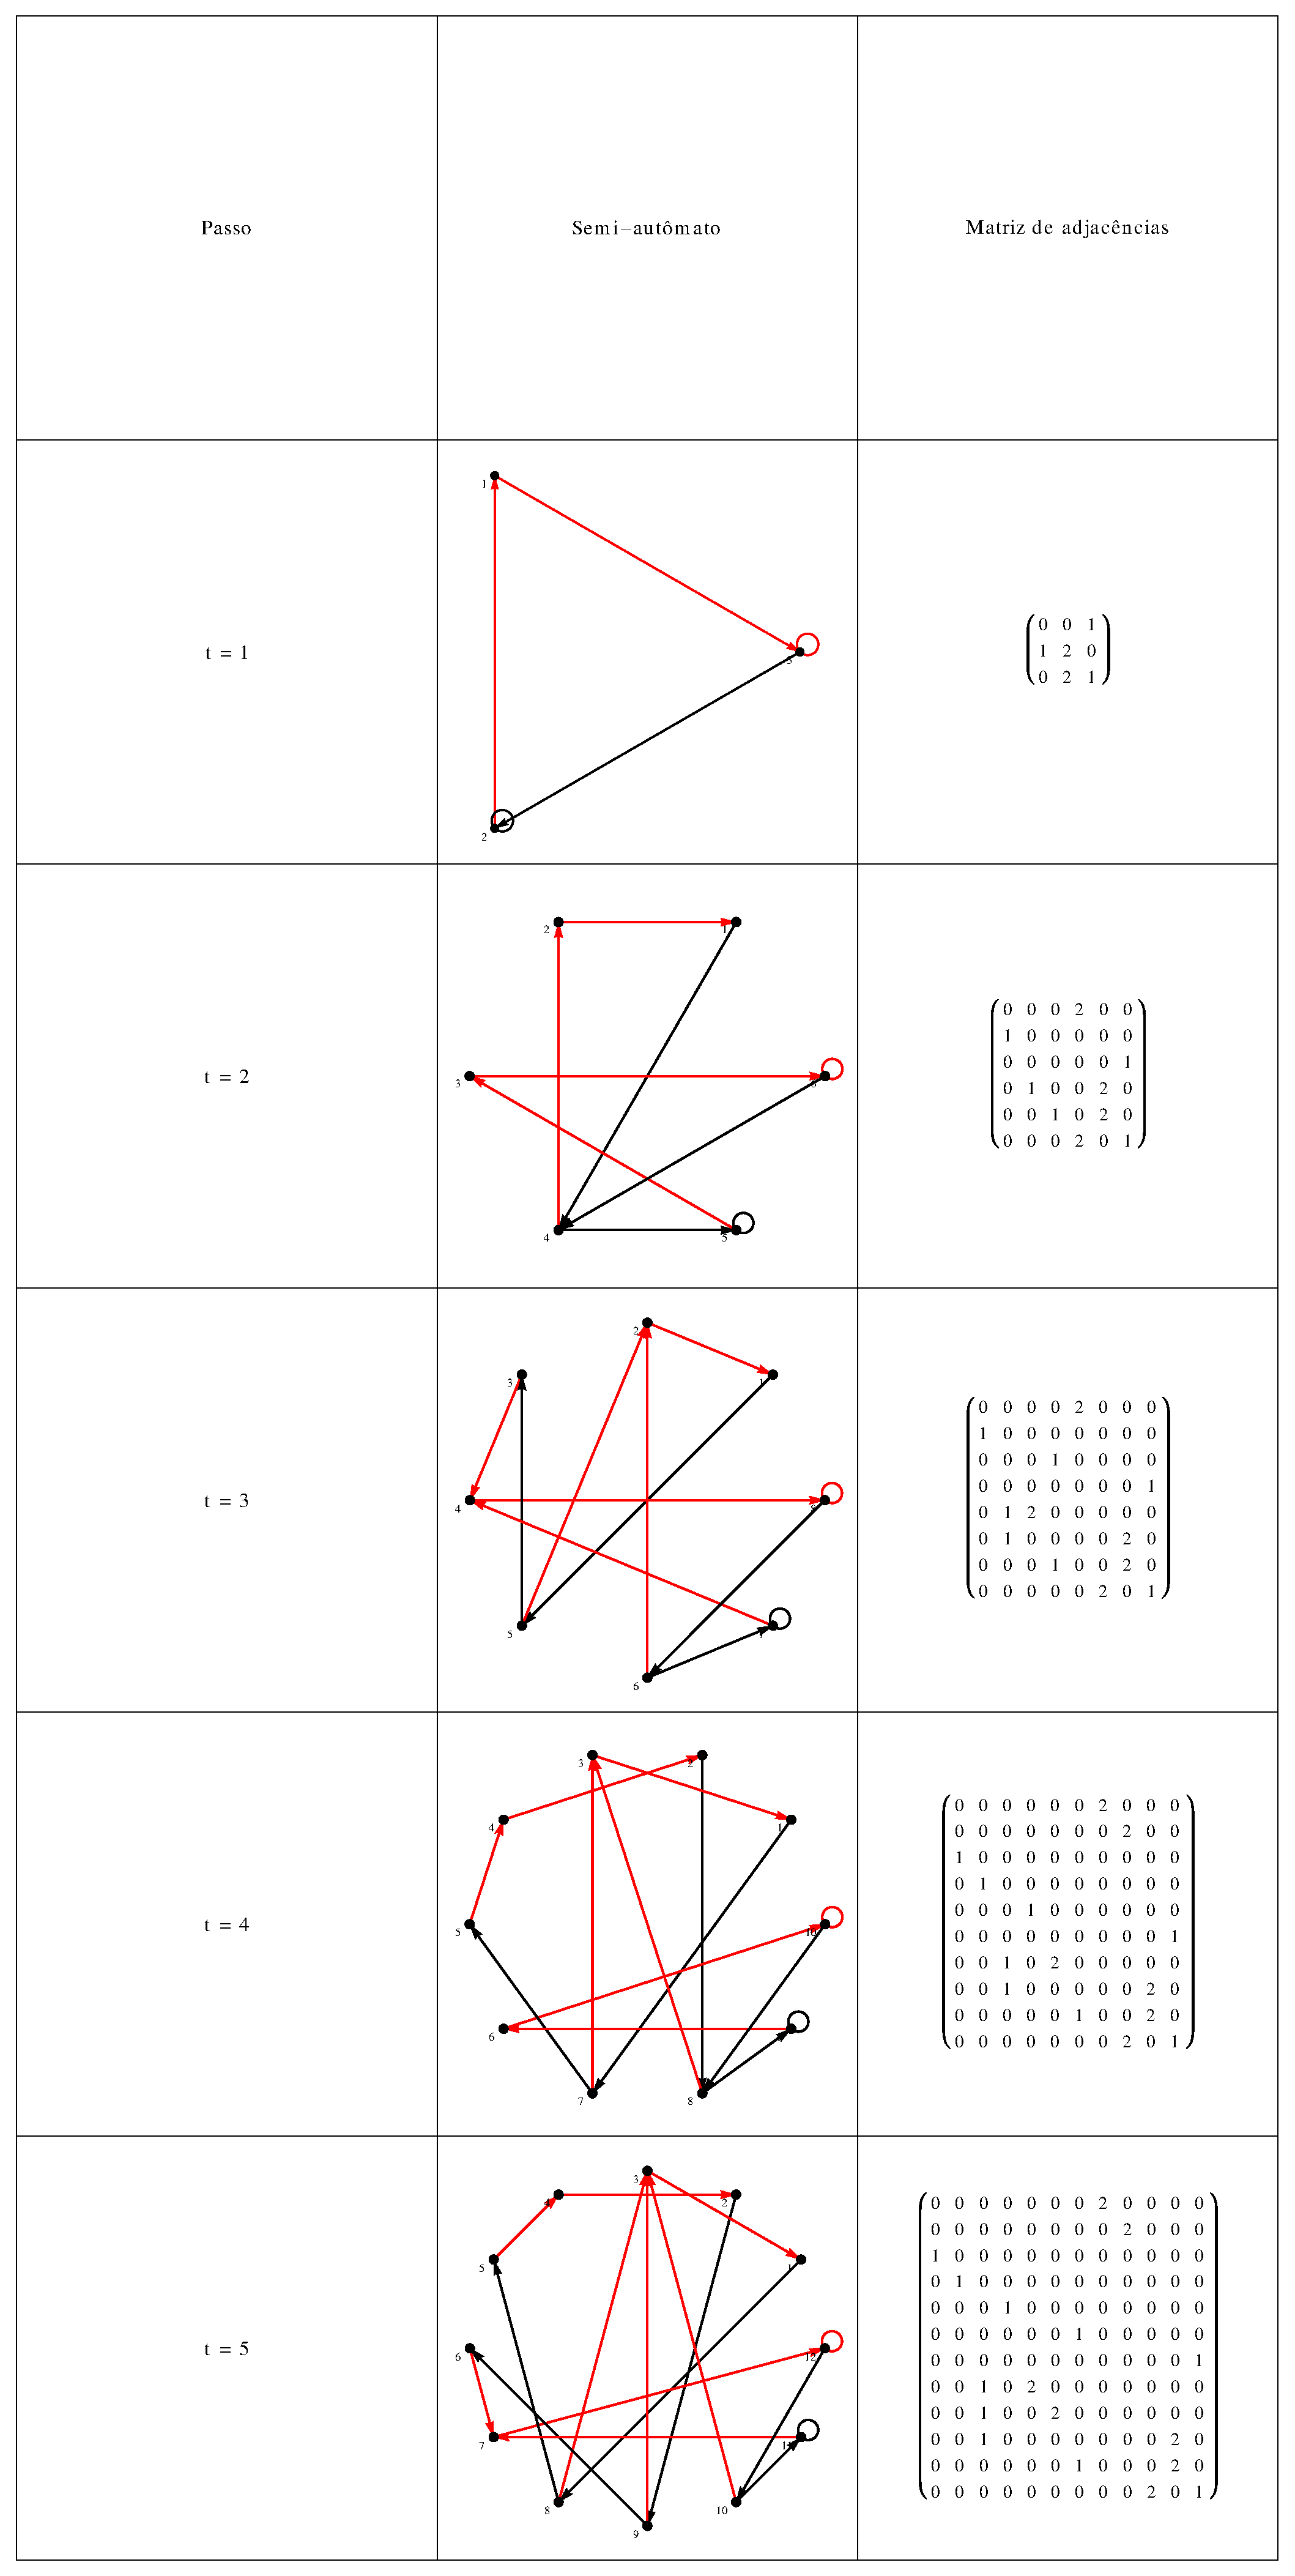
\includegraphics[scale=0.32]{img/mat/matr11.eps}
\caption{Regra 11.}
\label{tab:mr11}
\end{center}
\end{table}

\begin{table}[H]
\begin{center}
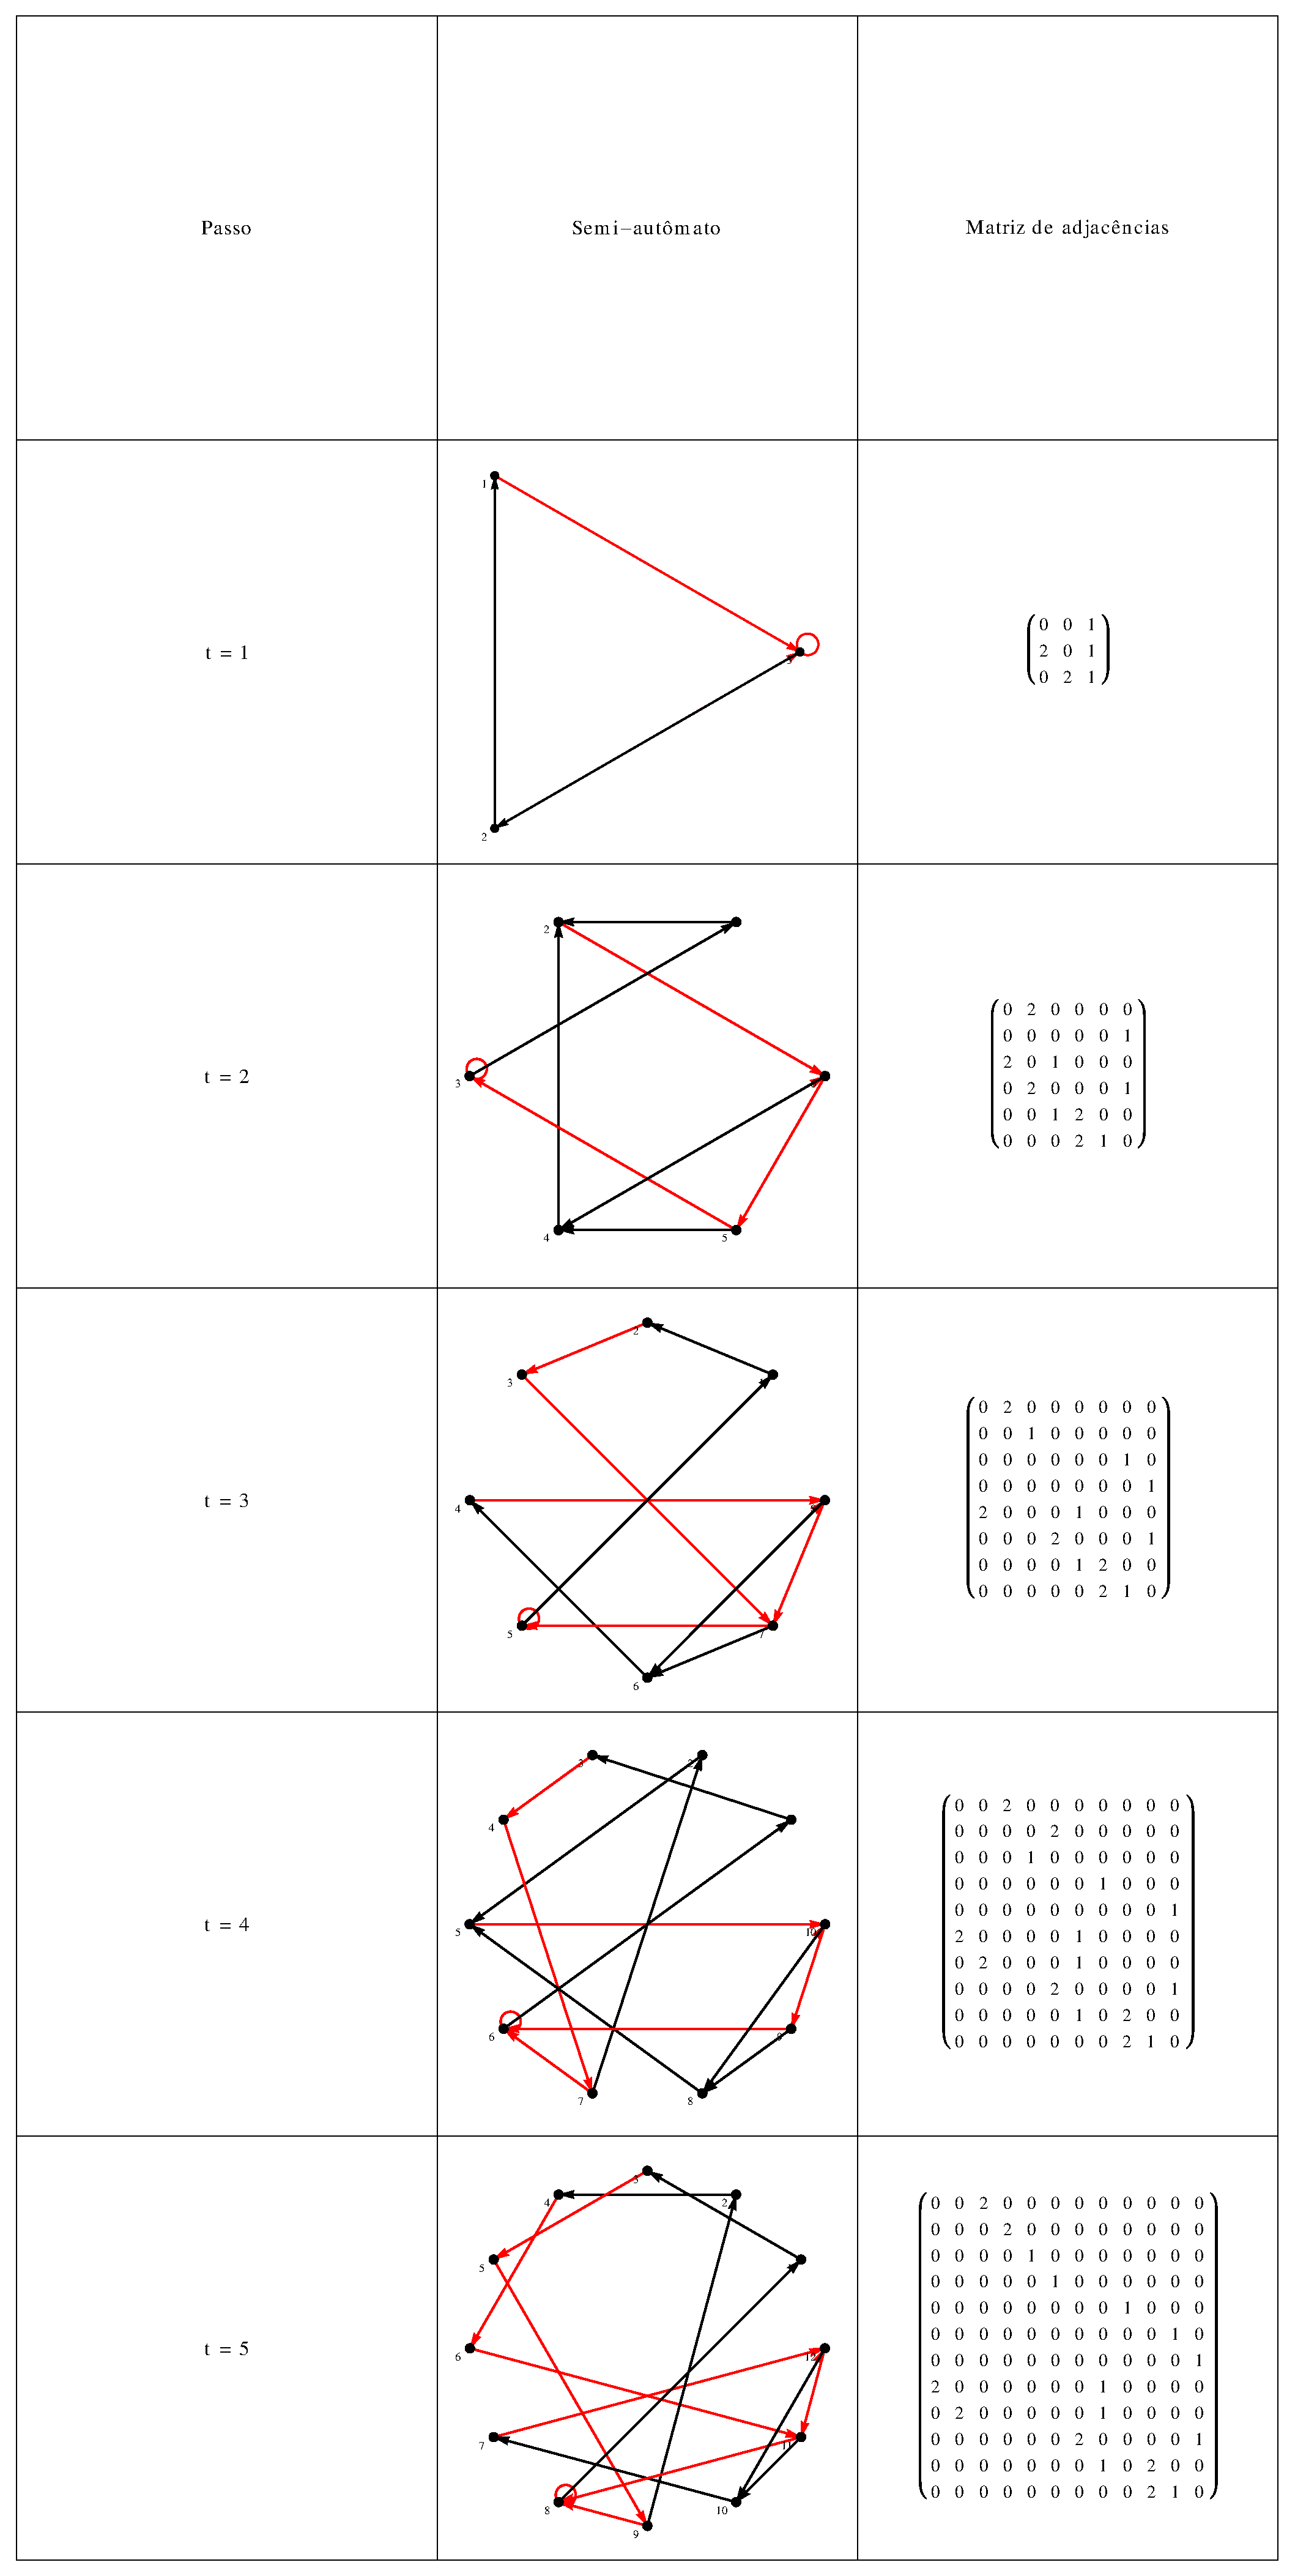
\includegraphics[scale=0.32]{img/mat/matr14.eps}
\caption{Regra 14.}
\label{tab:mr14}
\end{center}
\end{table}

\begin{table}[H]
\begin{center}
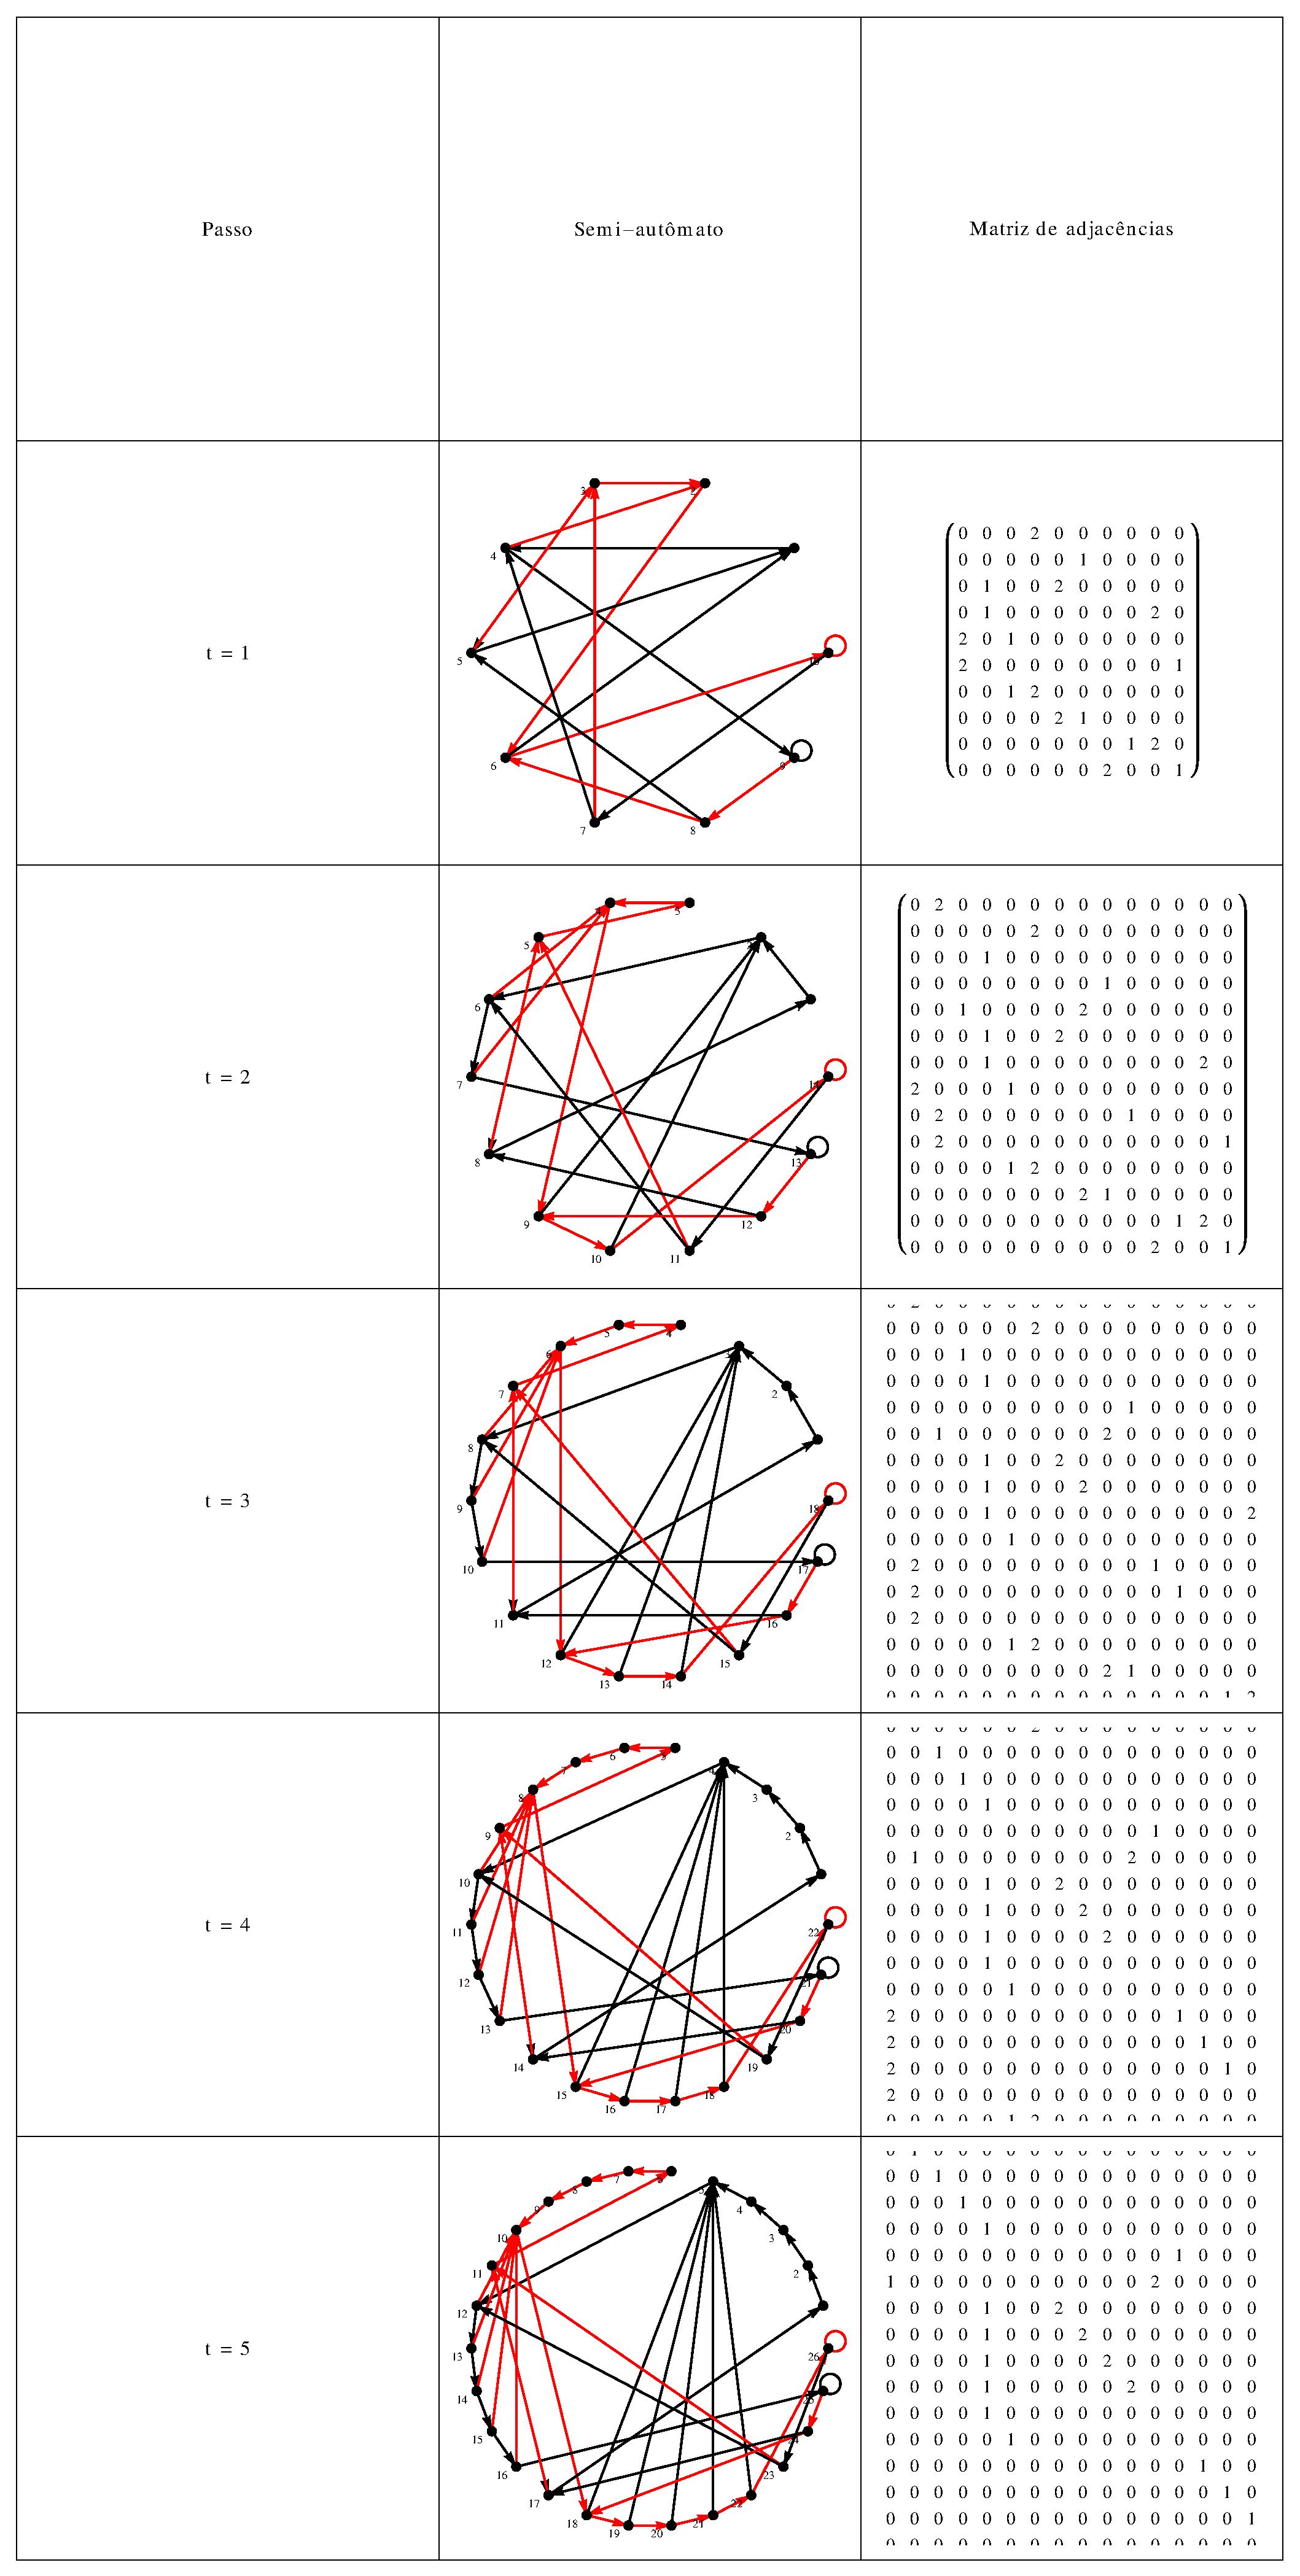
\includegraphics[scale=0.32]{img/mat/matr23.eps}
\caption{Regra 23.}
\label{tab:mr23}
\end{center}
\end{table}

\begin{table}[H]
\begin{center}
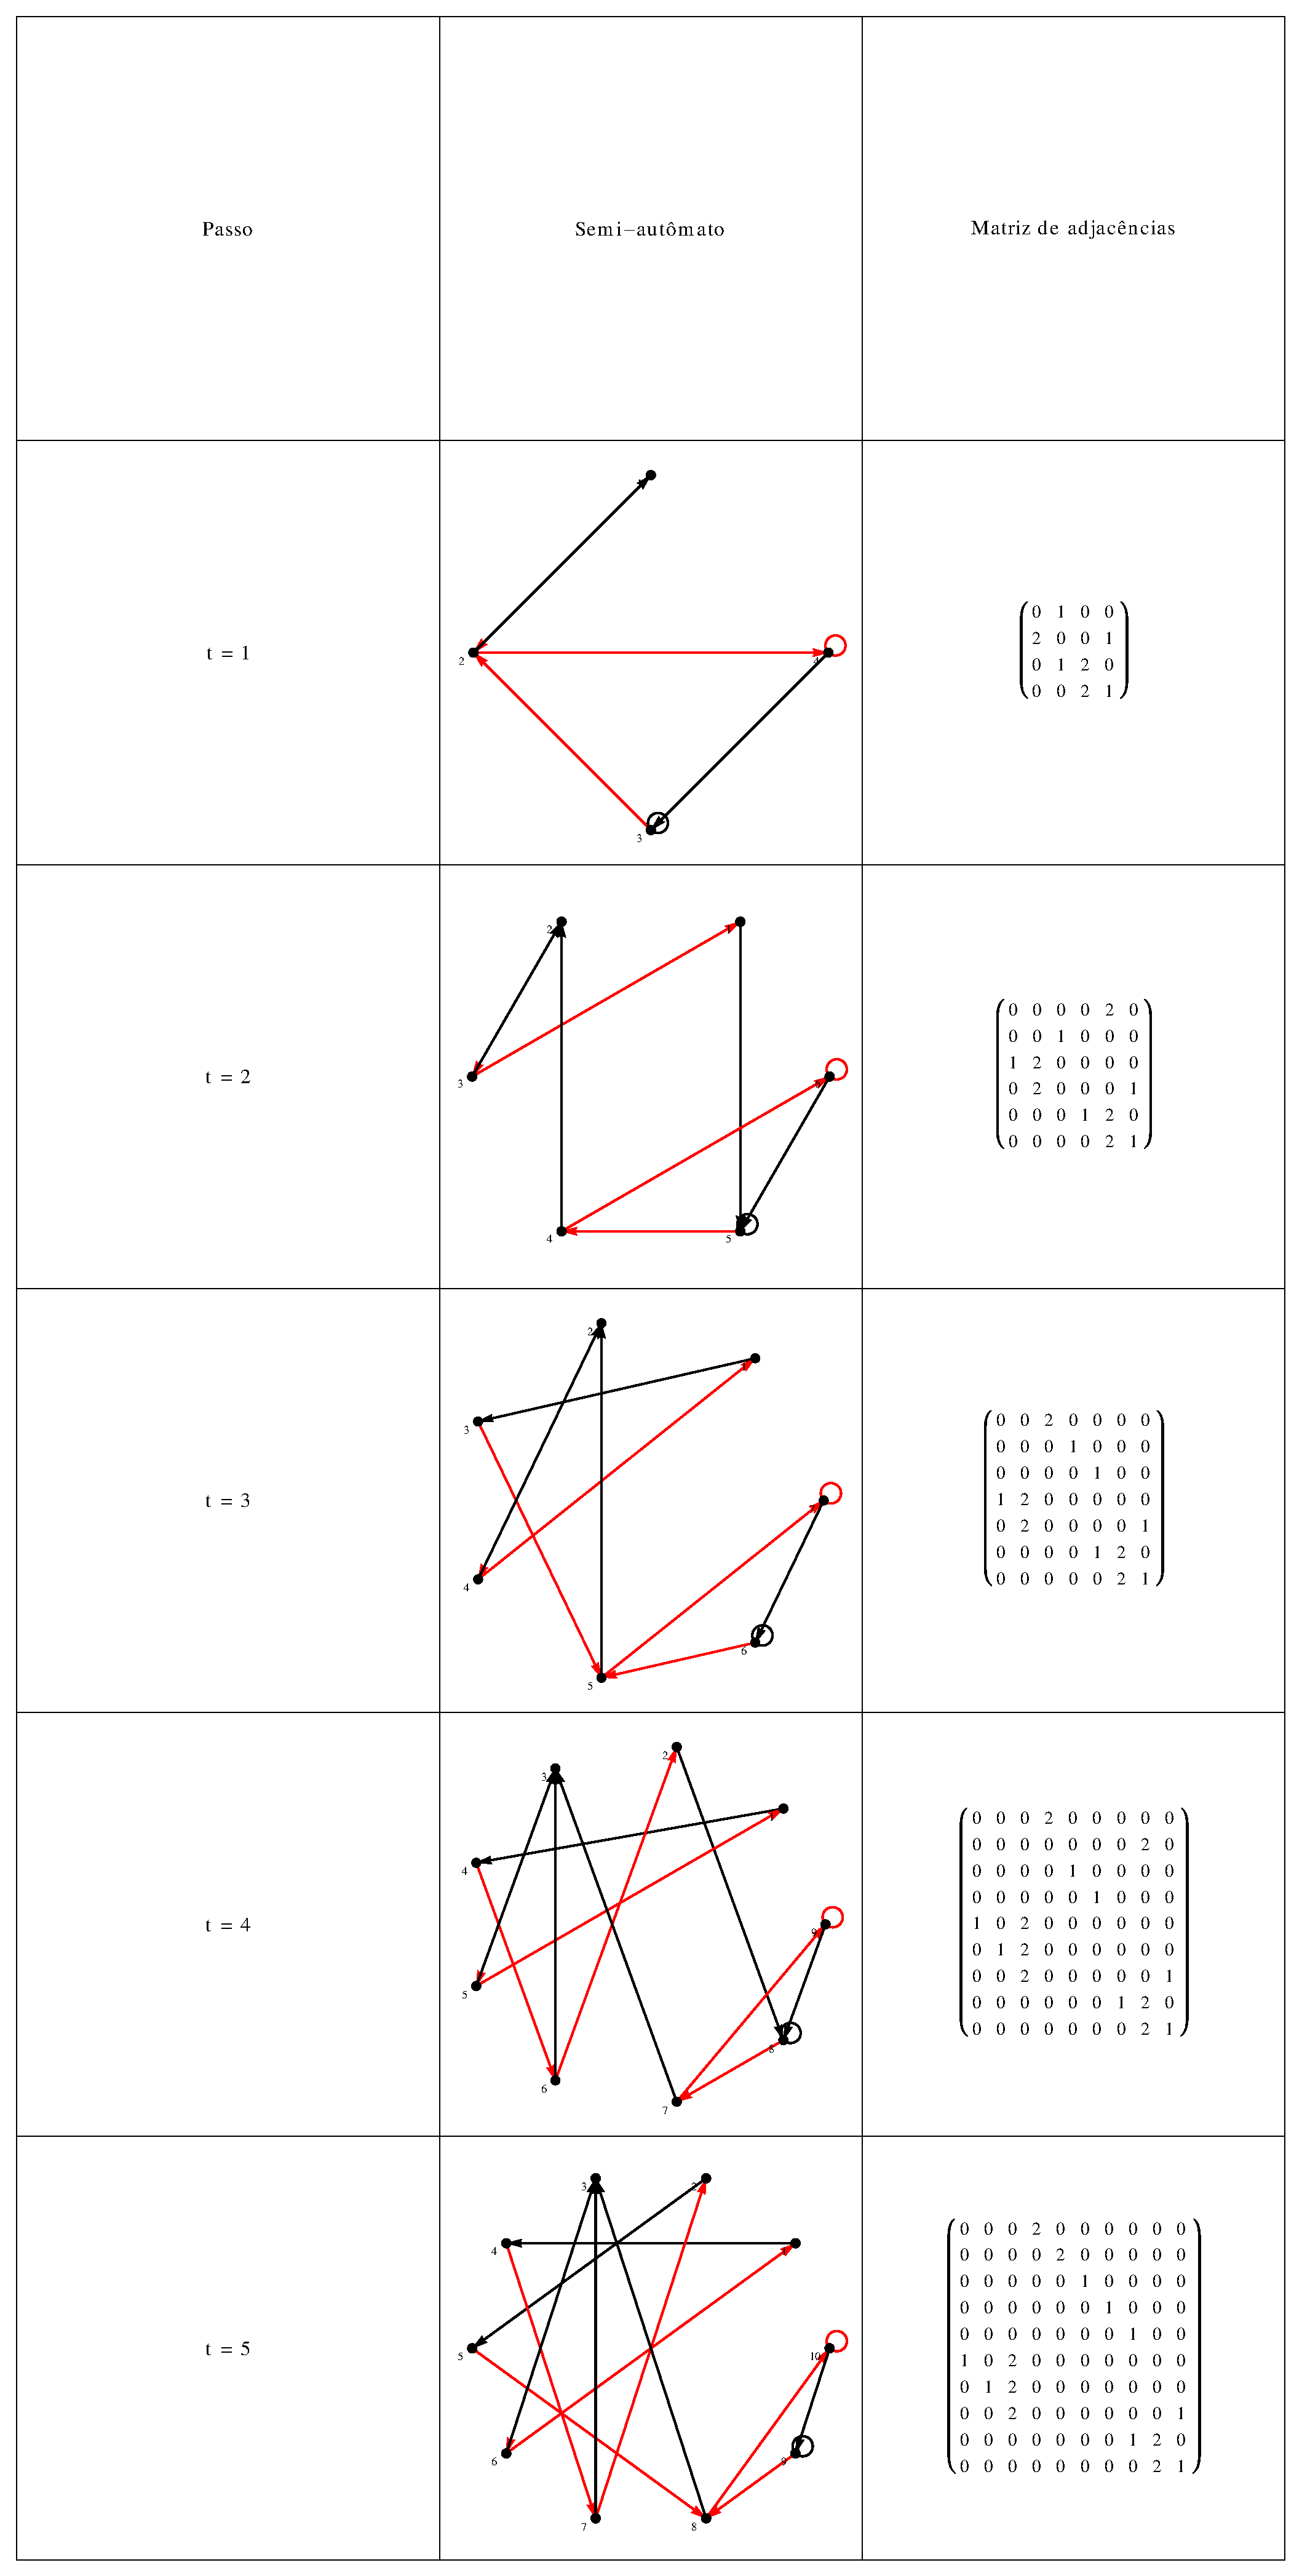
\includegraphics[scale=0.32]{img/mat/matr35.eps}
\caption{Regra 35.}
\label{tab:mr35}
\end{center}
\end{table}

\begin{table}[H]
\begin{center}
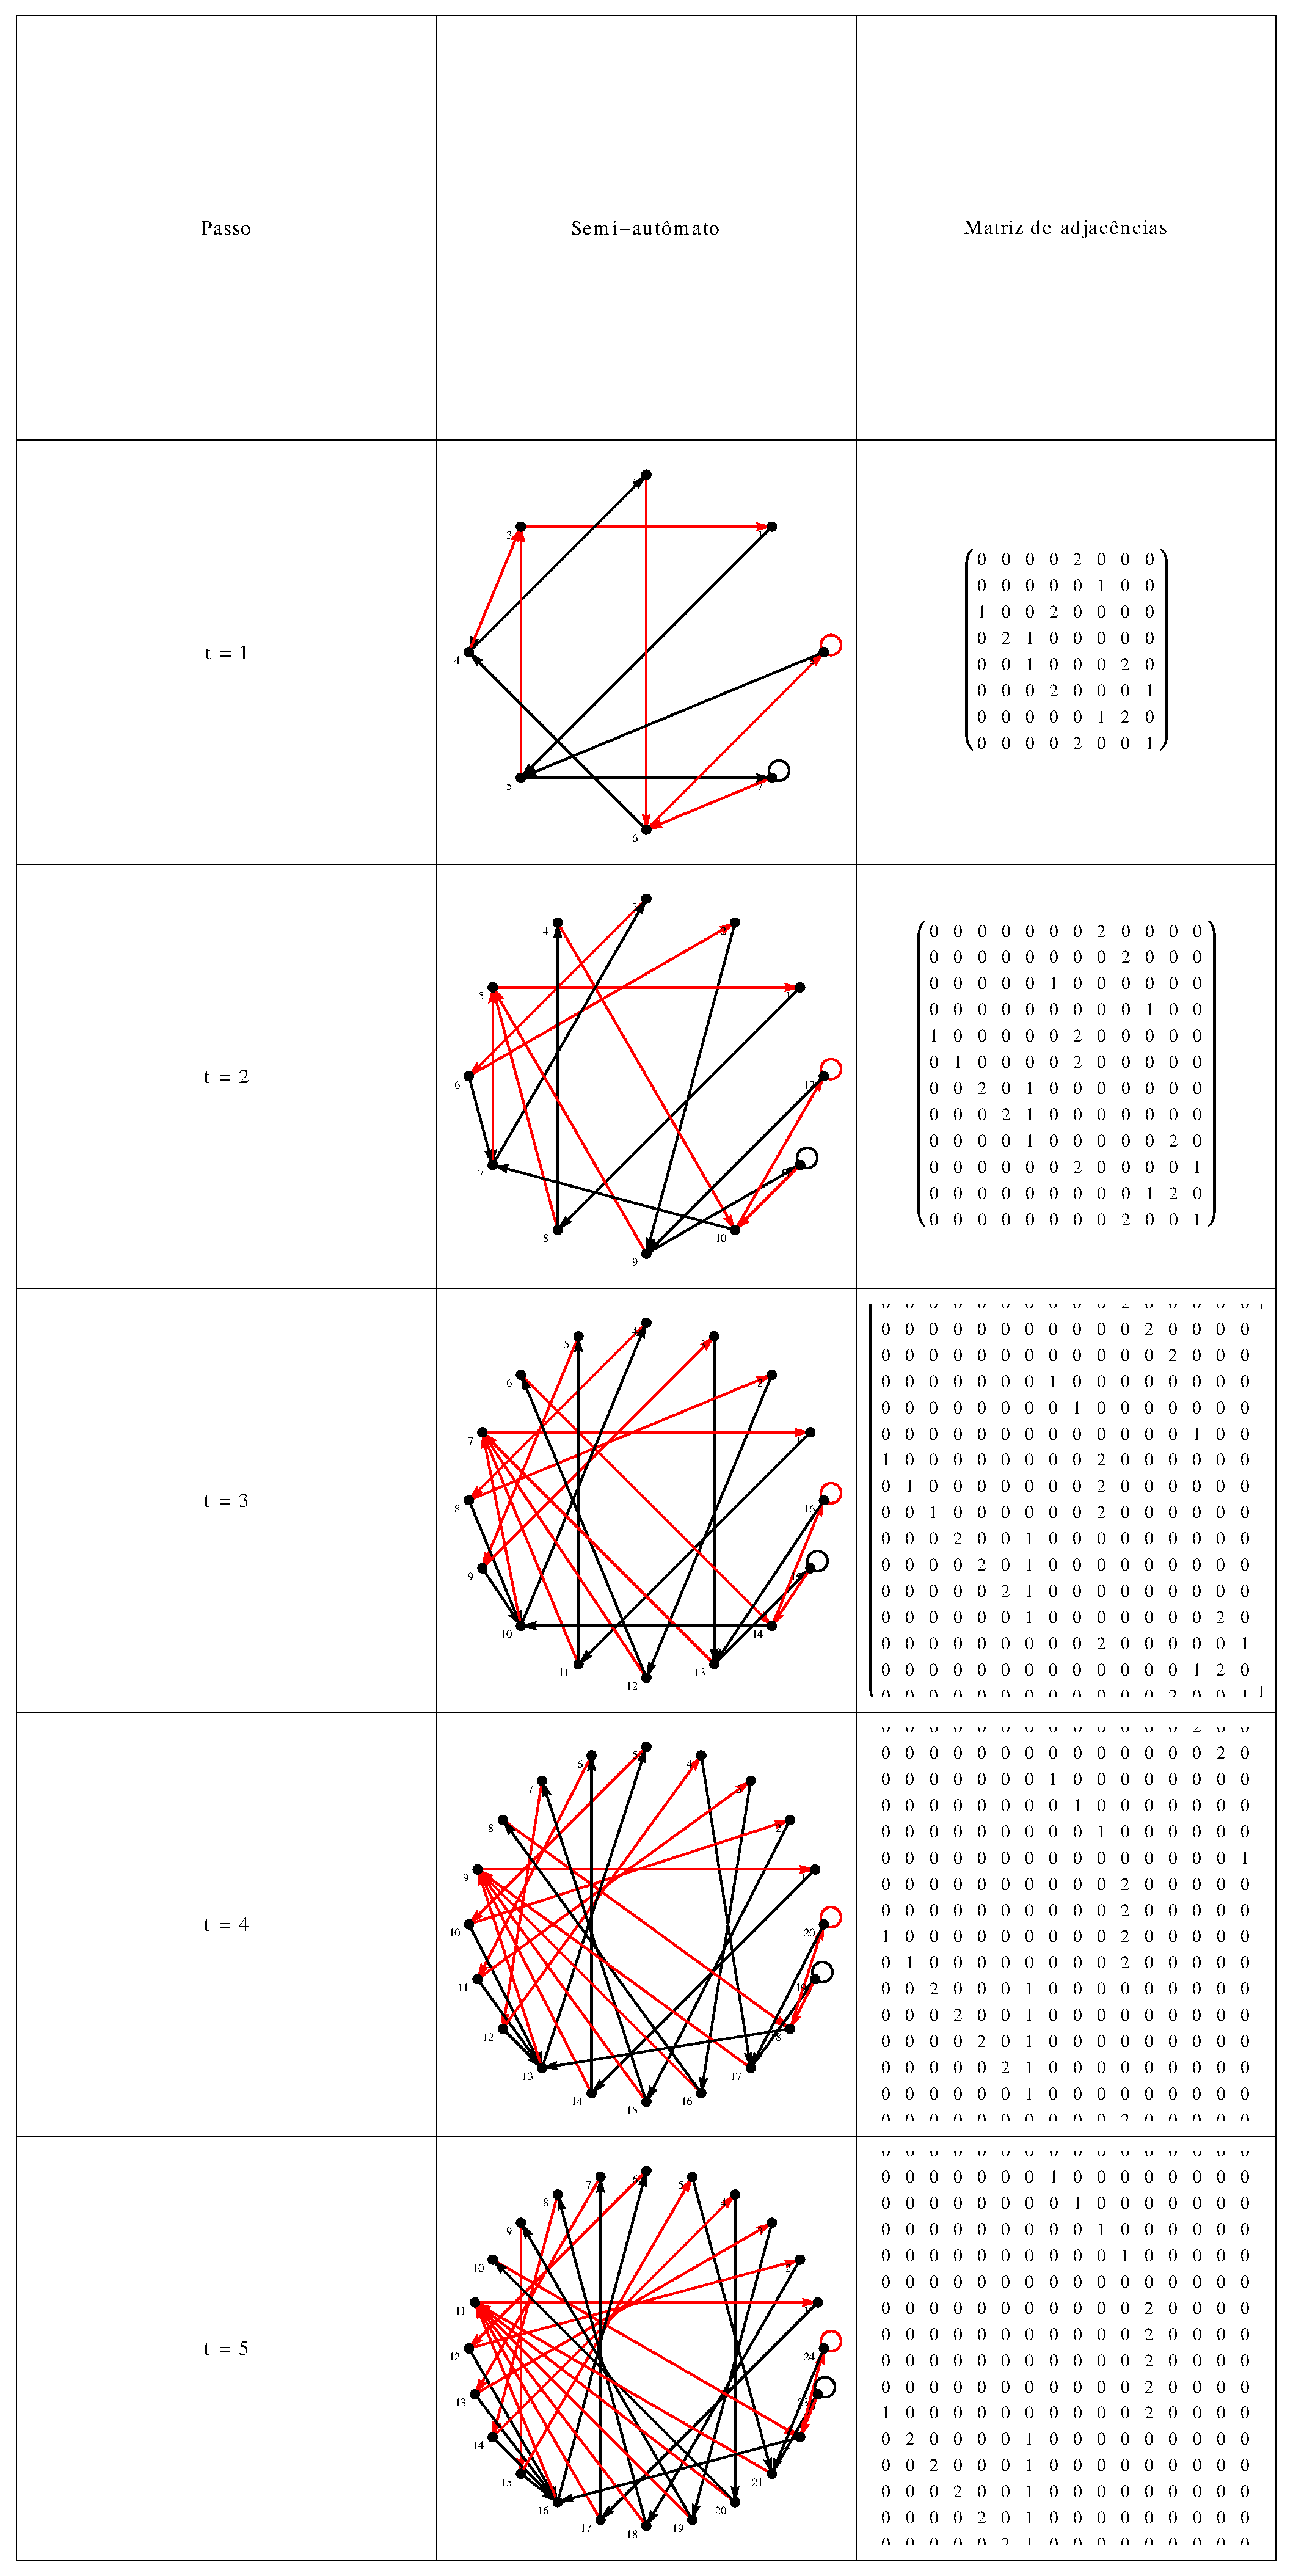
\includegraphics[scale=0.32]{img/mat/matr43.eps}
\caption{Regra 43.}
\label{tab:mr43}
\end{center}
\end{table}

\begin{table}[H]
\begin{center}
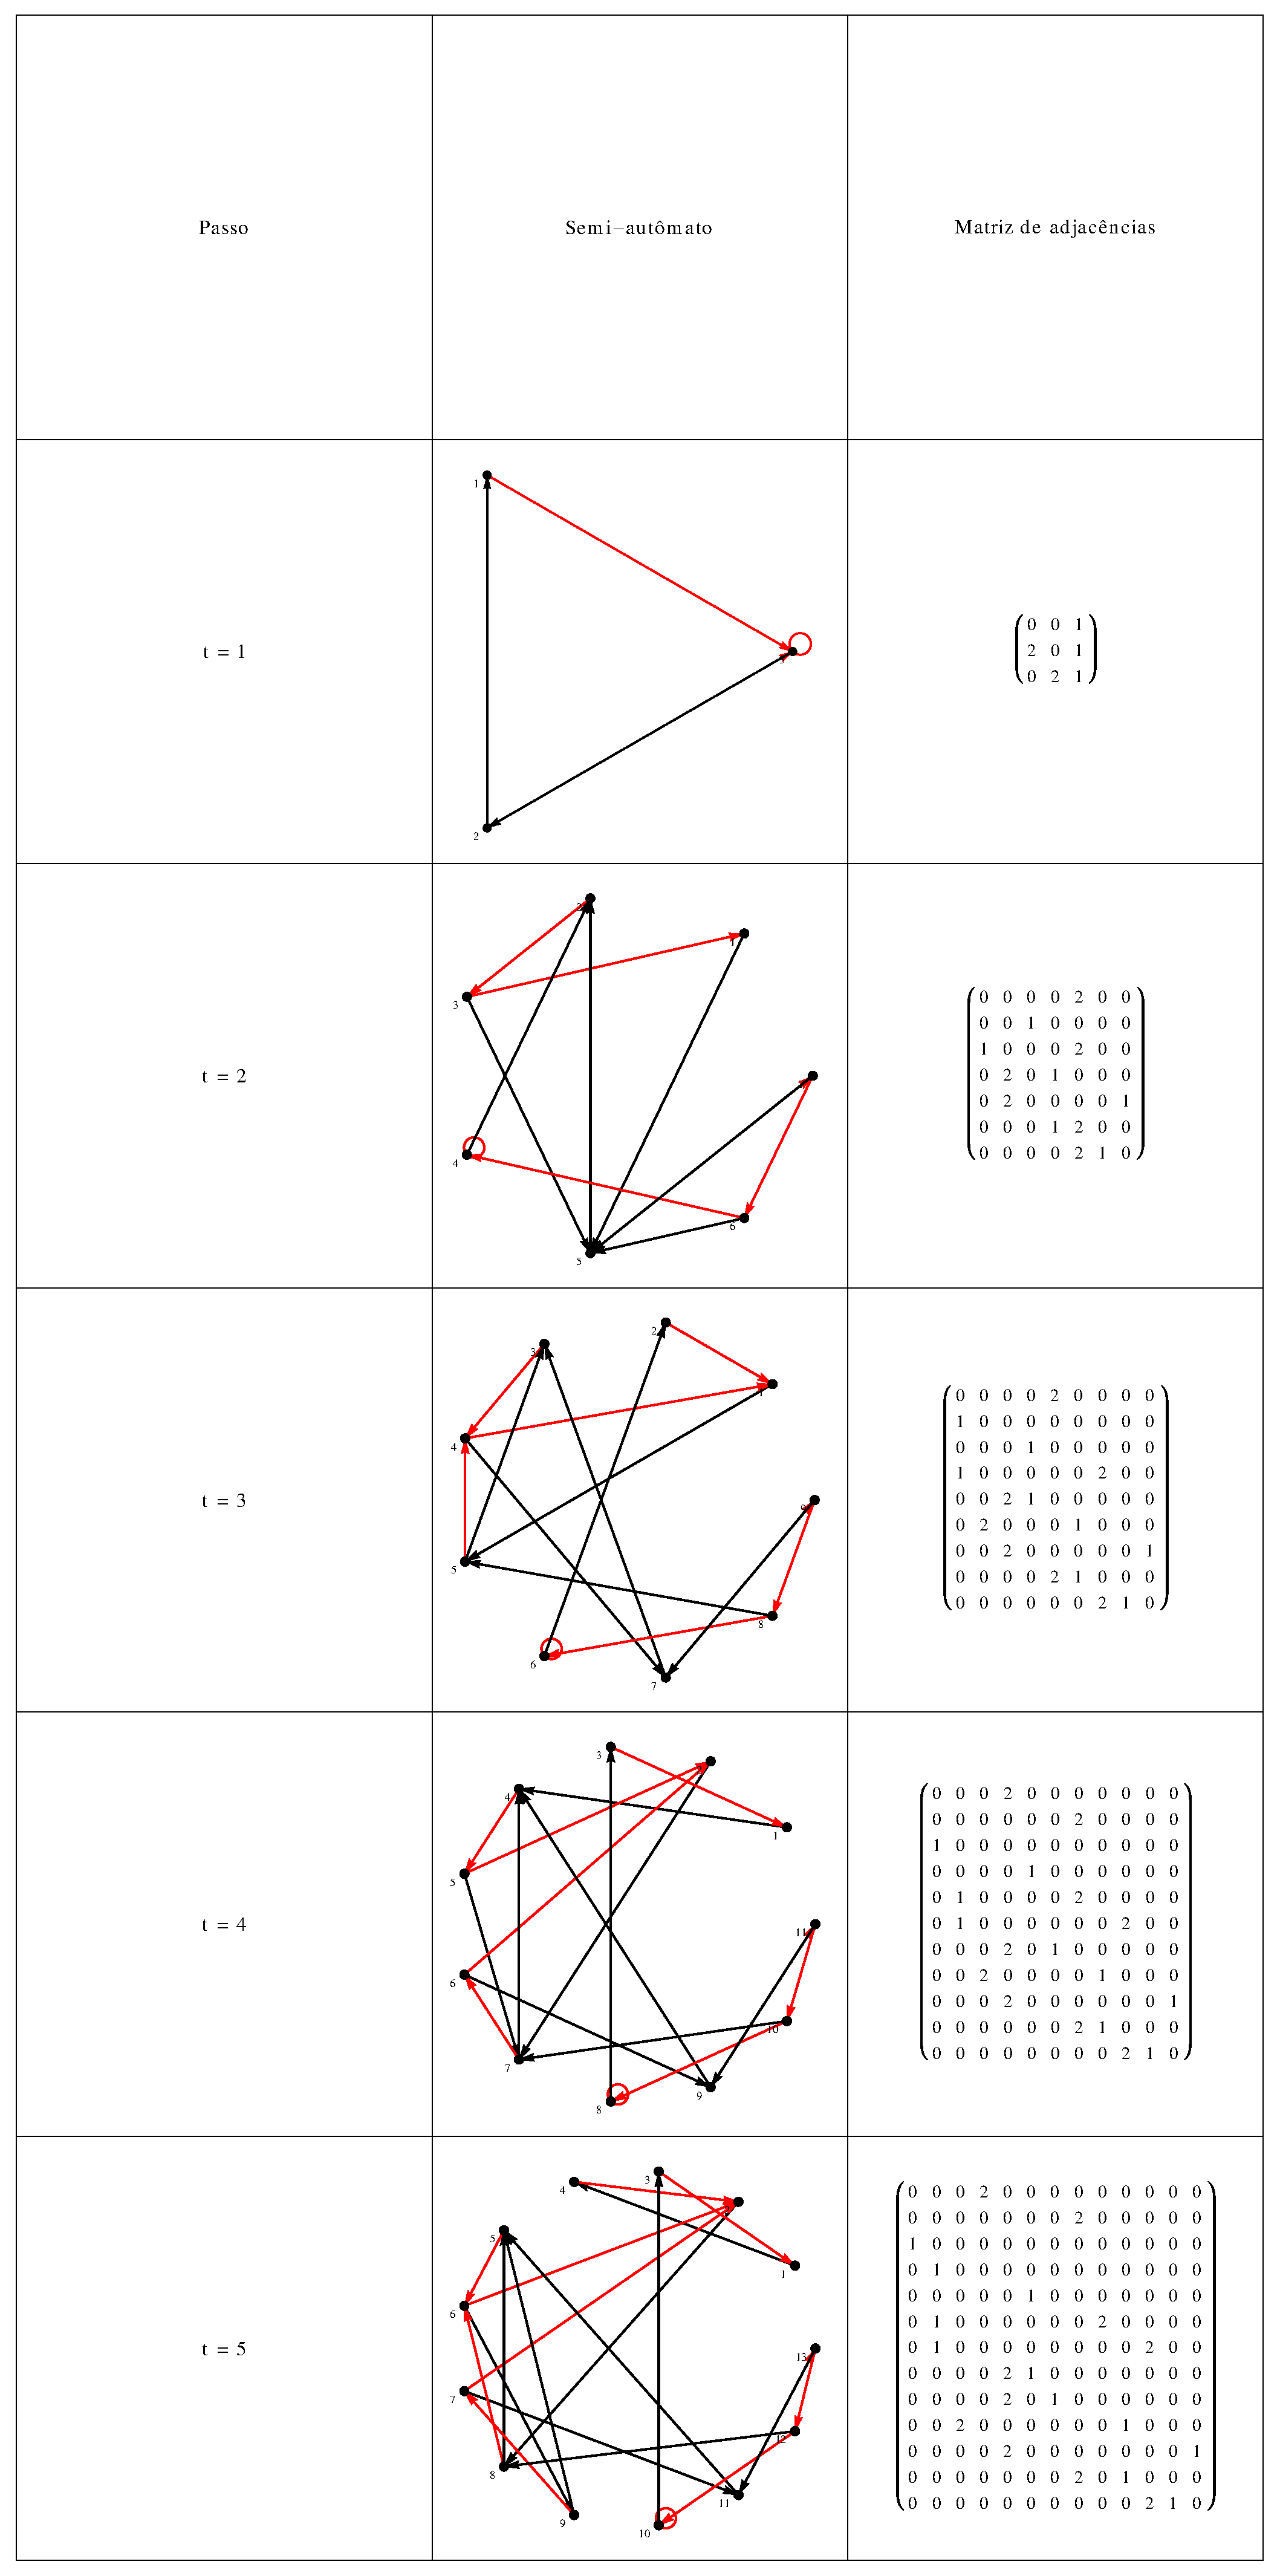
\includegraphics[scale=0.32]{img/mat/matr50.eps}
\caption{Regra 50.}
\label{tab:mr50}
\end{center}
\end{table}

\begin{table}[H]
\begin{center}
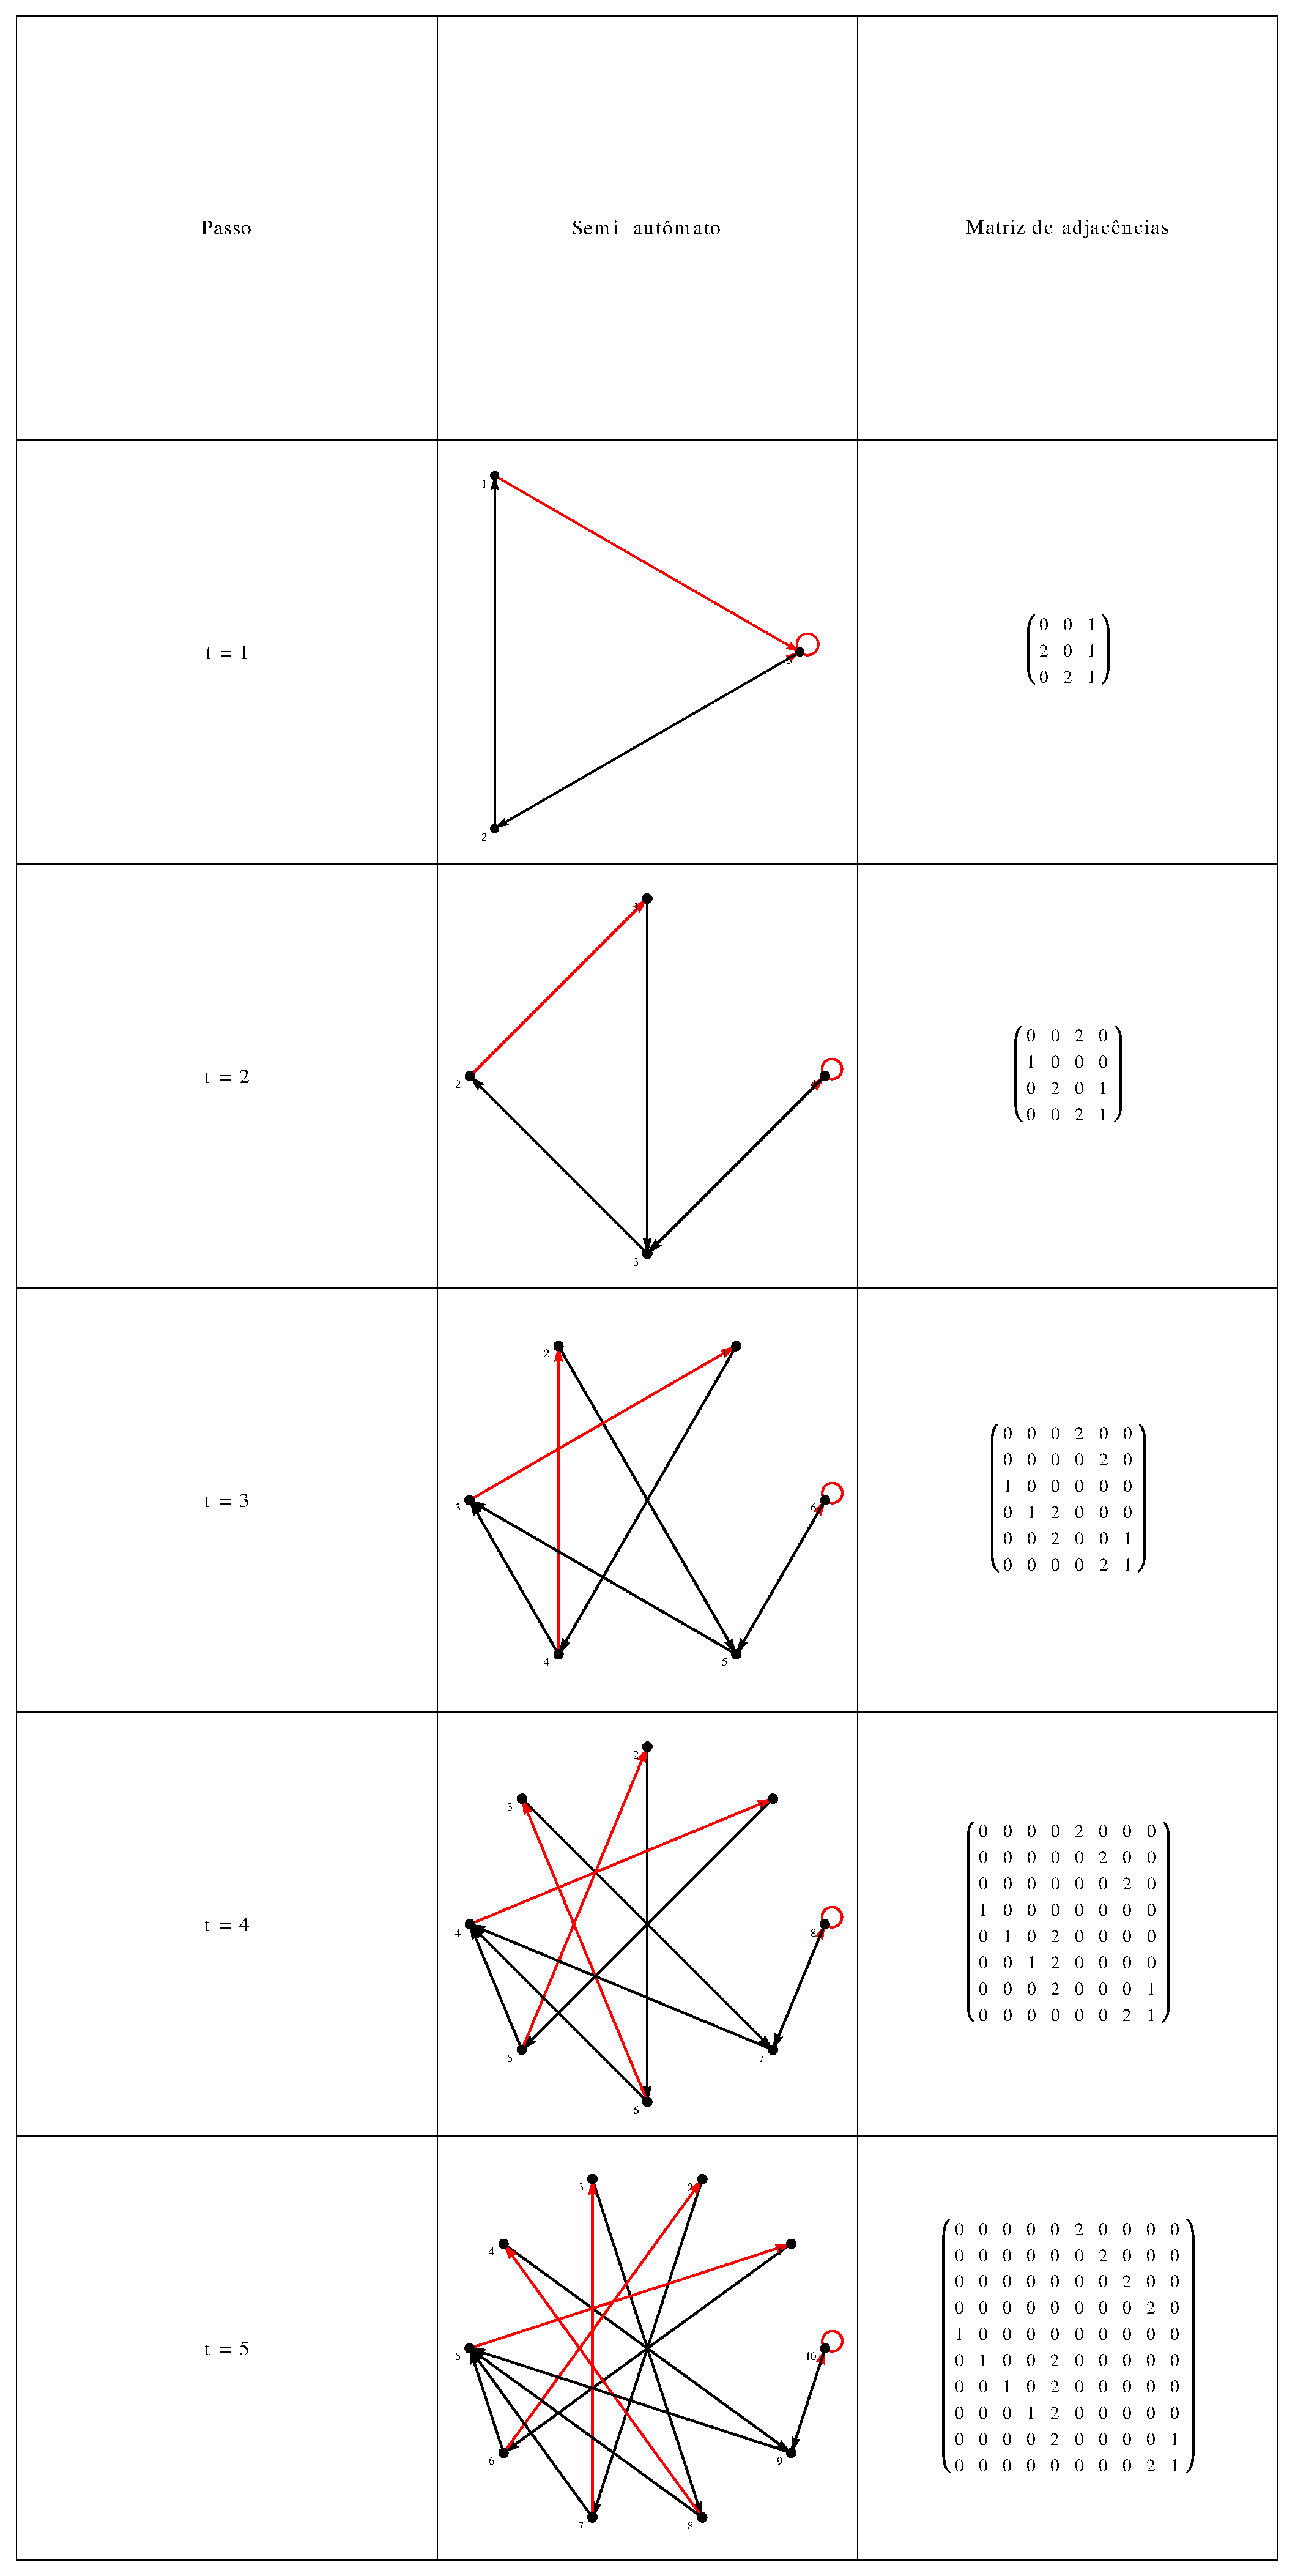
\includegraphics[scale=0.32]{img/mat/matr56.eps}
\caption{Regra 56.}
\label{tab:mr56}
\end{center}
\end{table}

\begin{table}[H]
\begin{center}
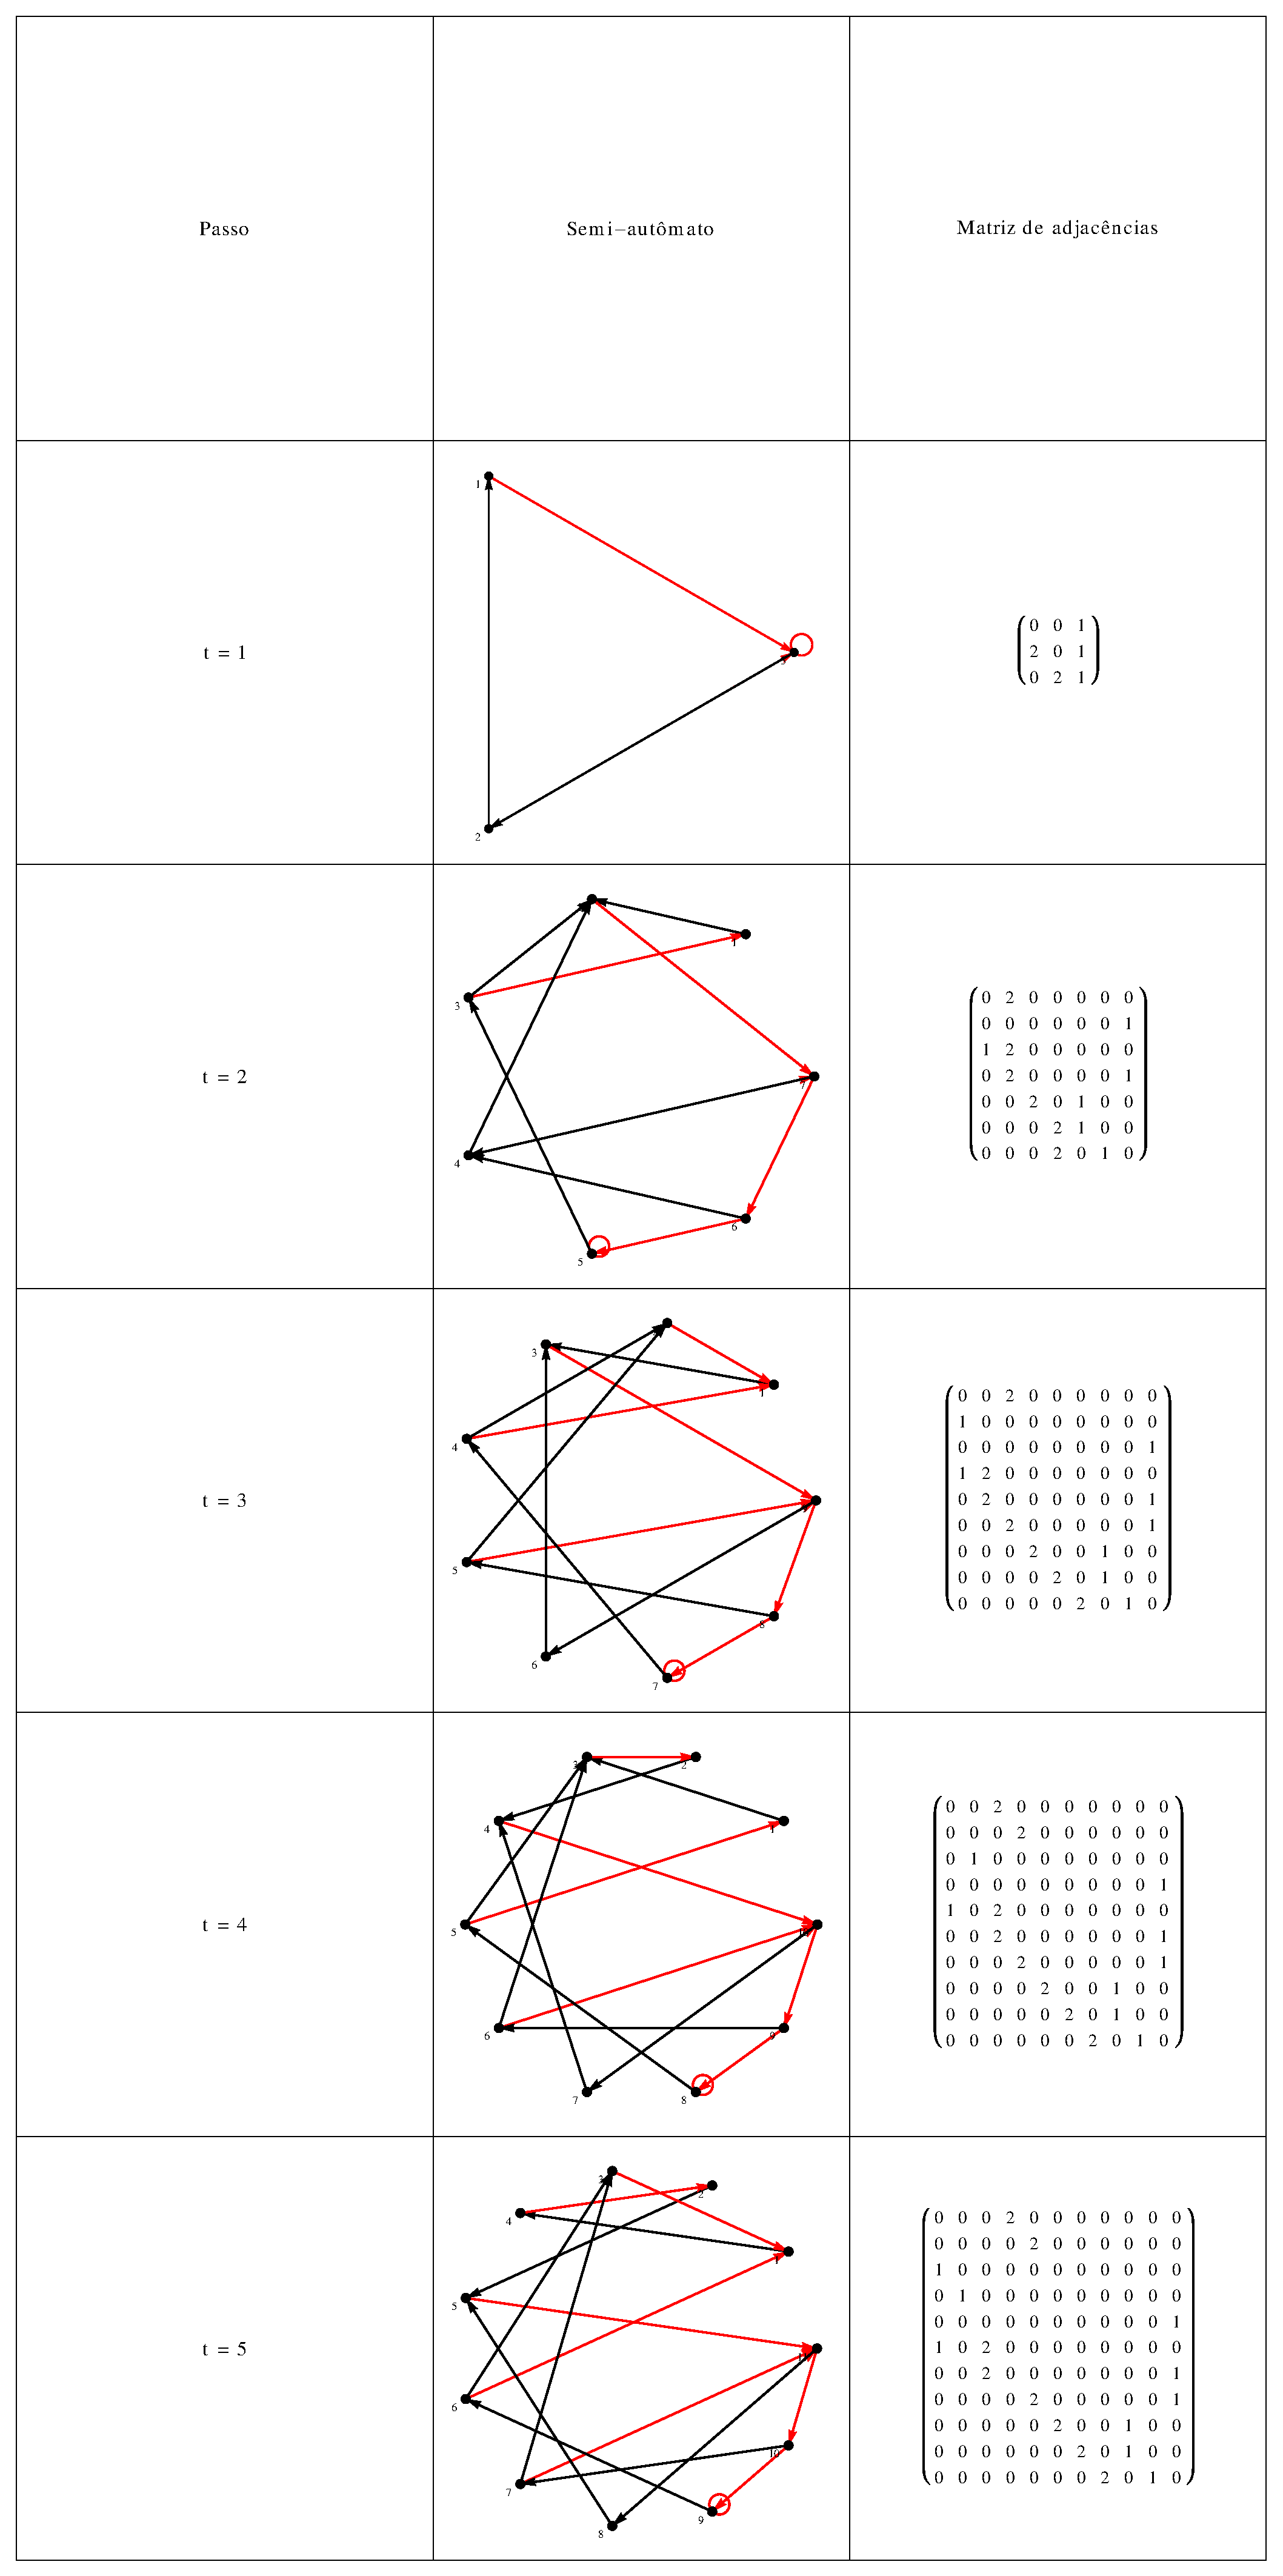
\includegraphics[scale=0.32]{img/mat/matr70.eps}
\caption{Regra 70.}
\label{tab:mr70}
\end{center}
\end{table}

\begin{table}[H]
\begin{center}
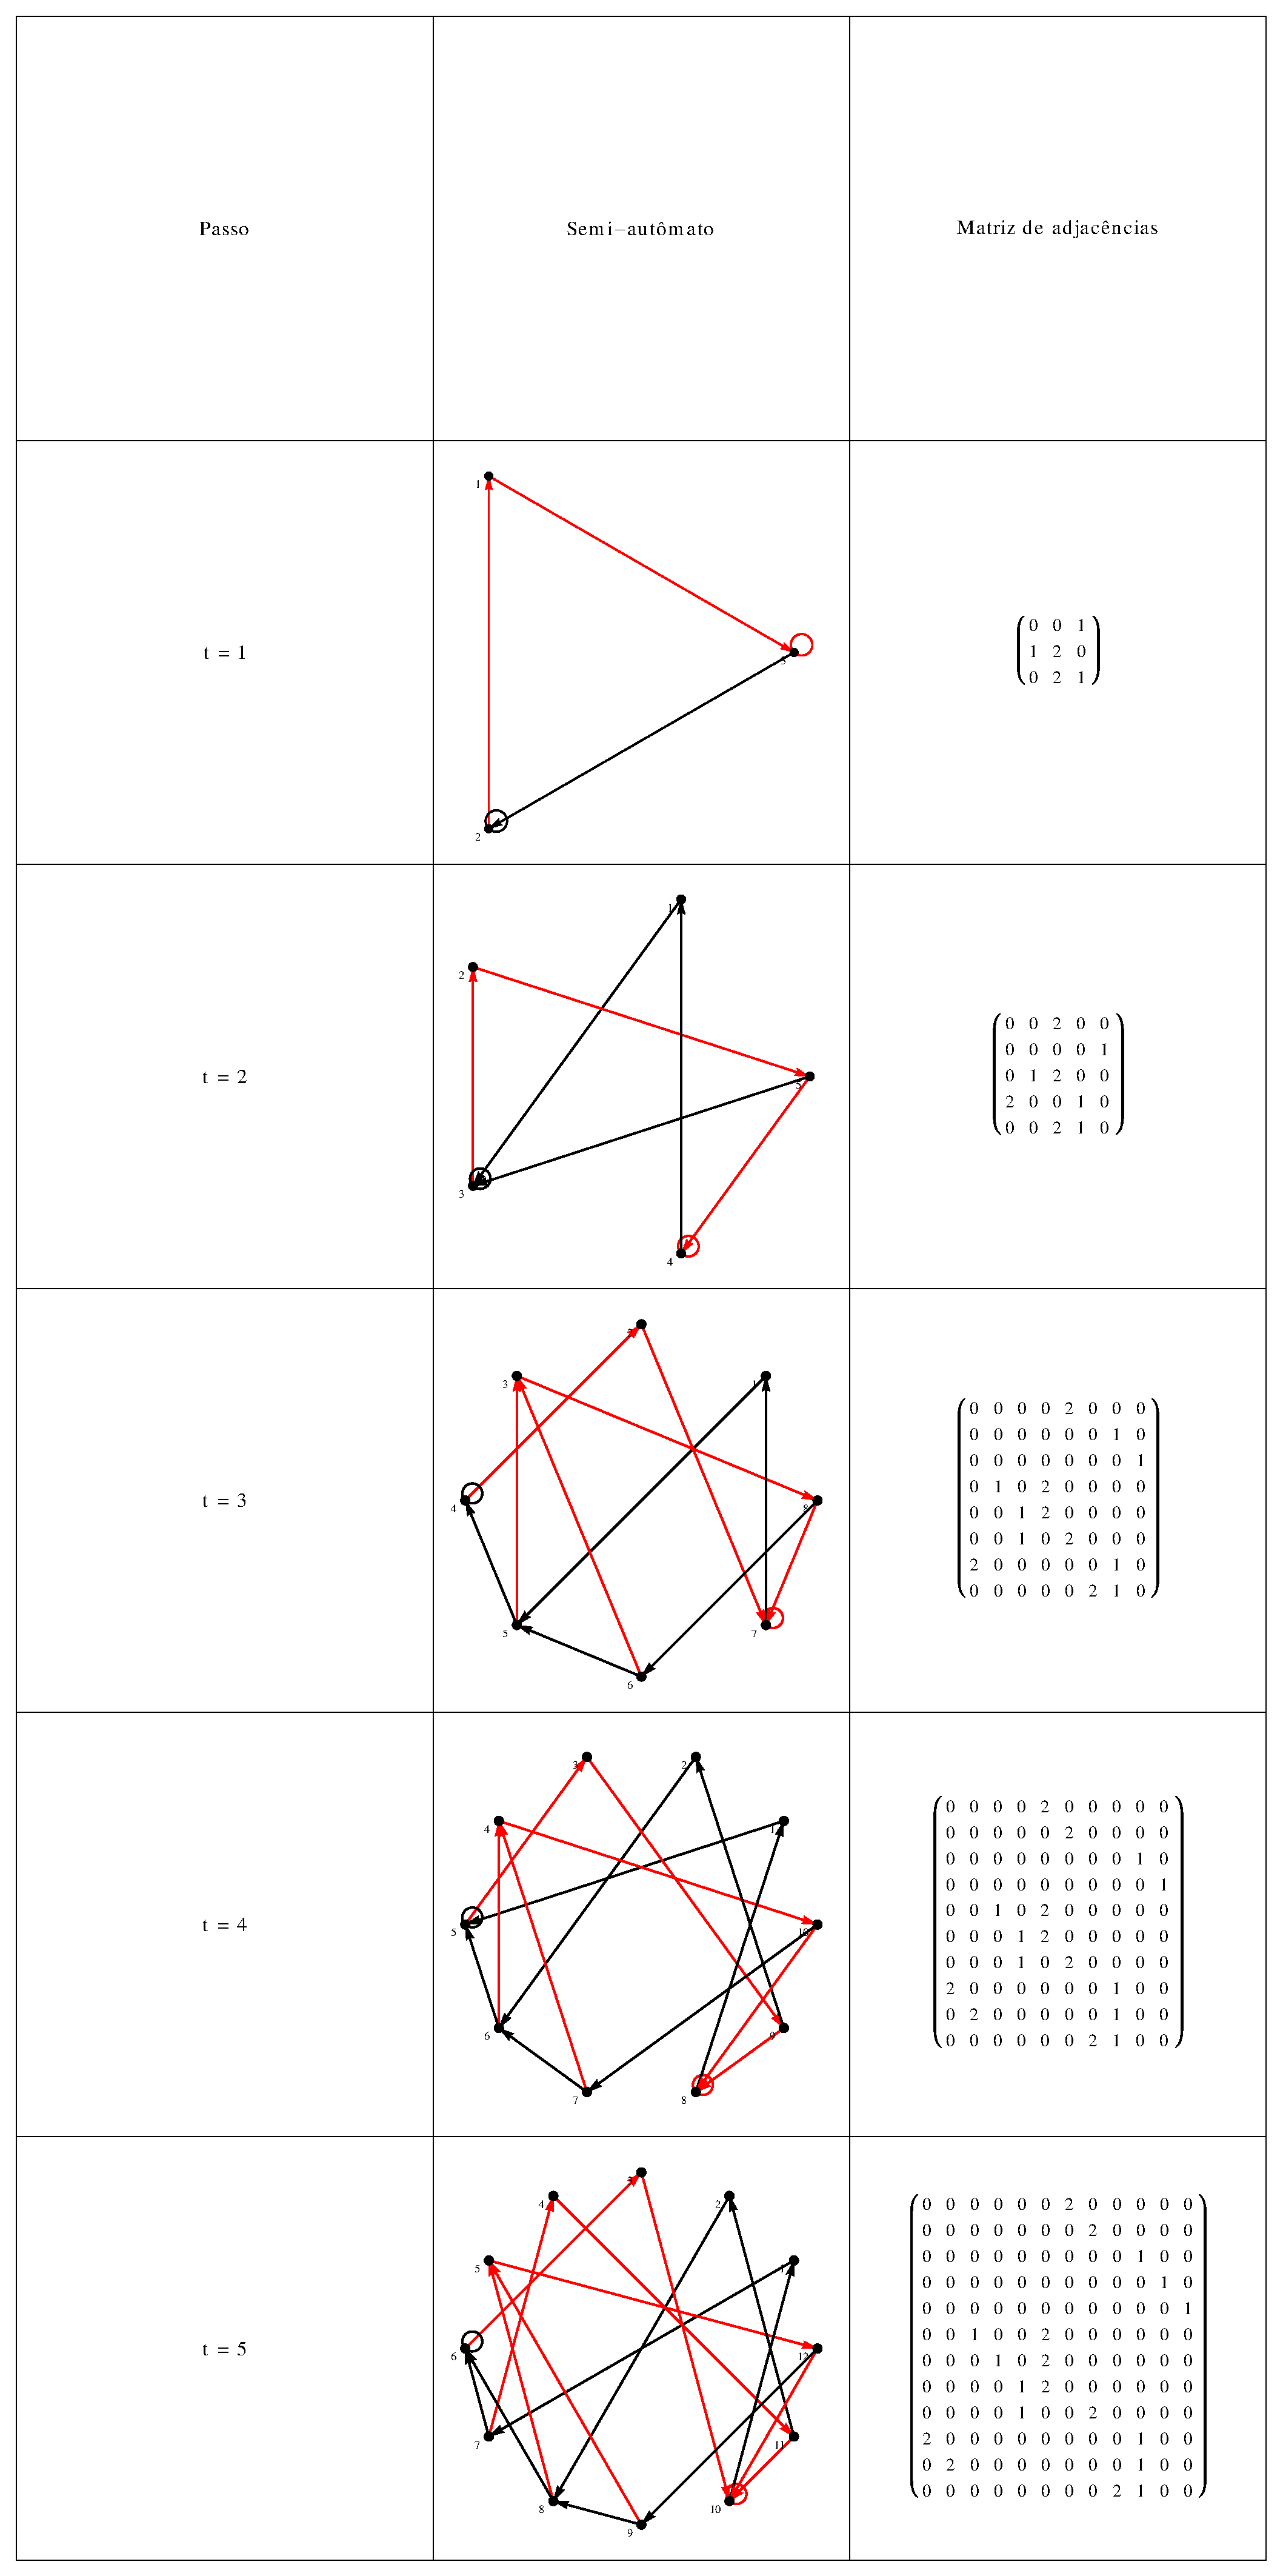
\includegraphics[scale=0.32]{img/mat/matr81.eps}
\caption{Regra 81.}
\label{tab:mr81}
\end{center}
\end{table}

\begin{table}[H]
\begin{center}
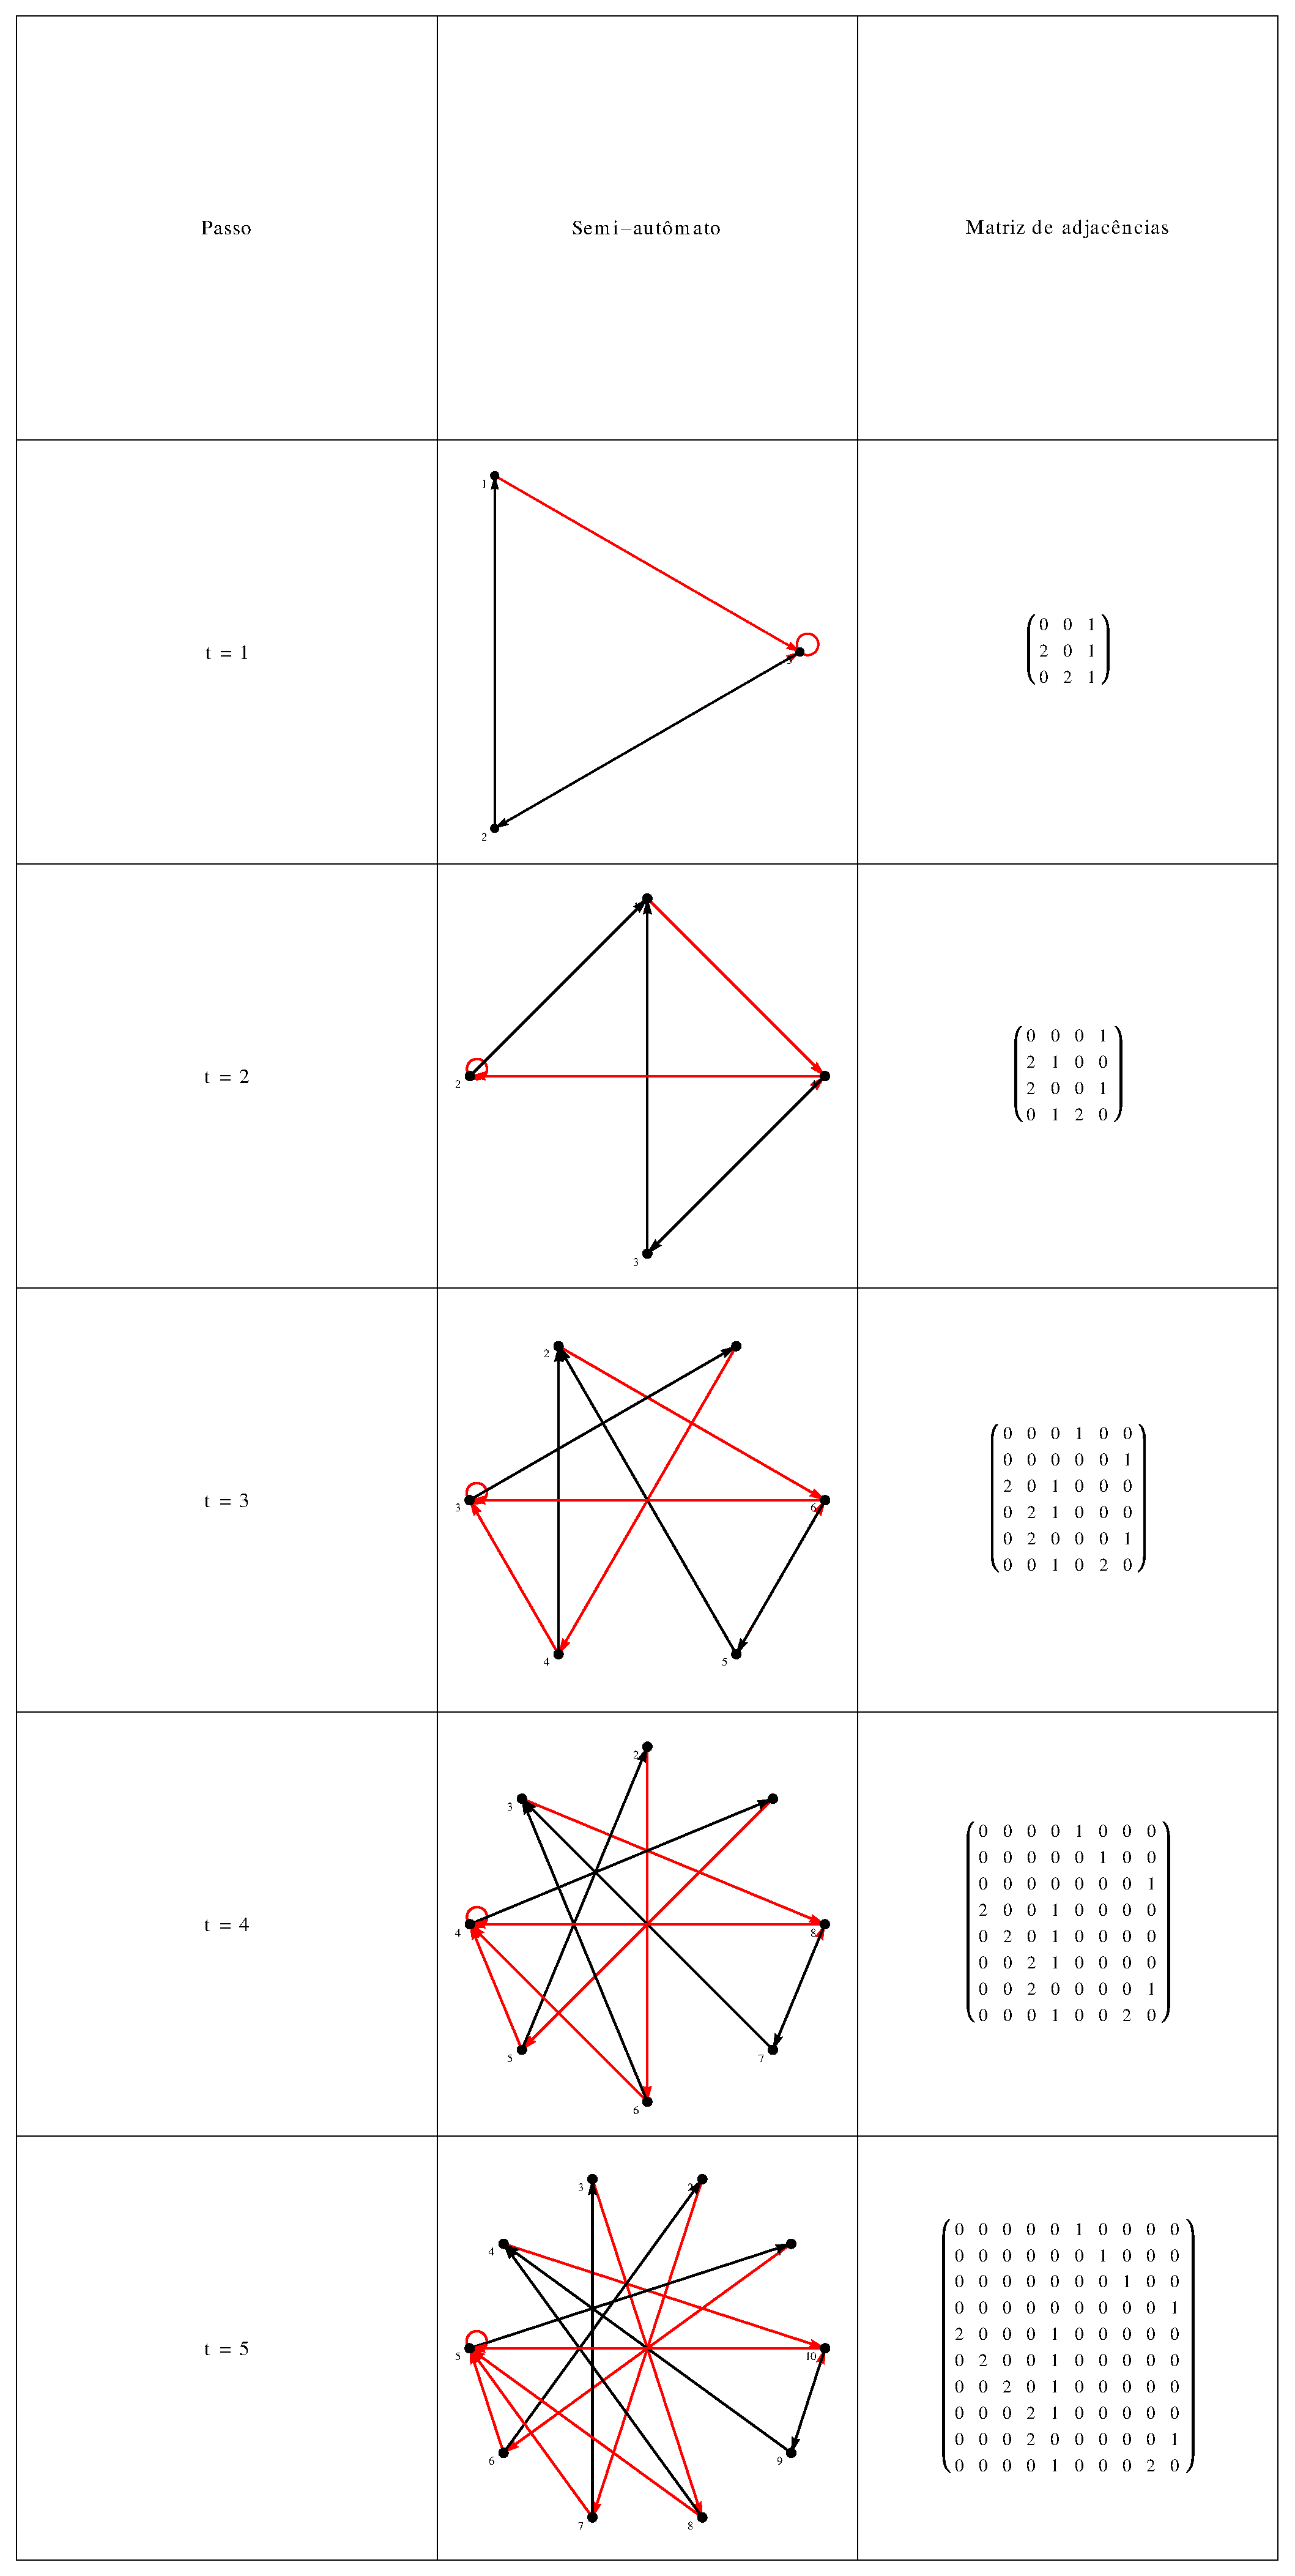
\includegraphics[scale=0.32]{img/mat/matr98.eps}
\caption{Regra 98.}
\label{tab:mr98}
\end{center}
\end{table}

\begin{table}[H]
\begin{center}
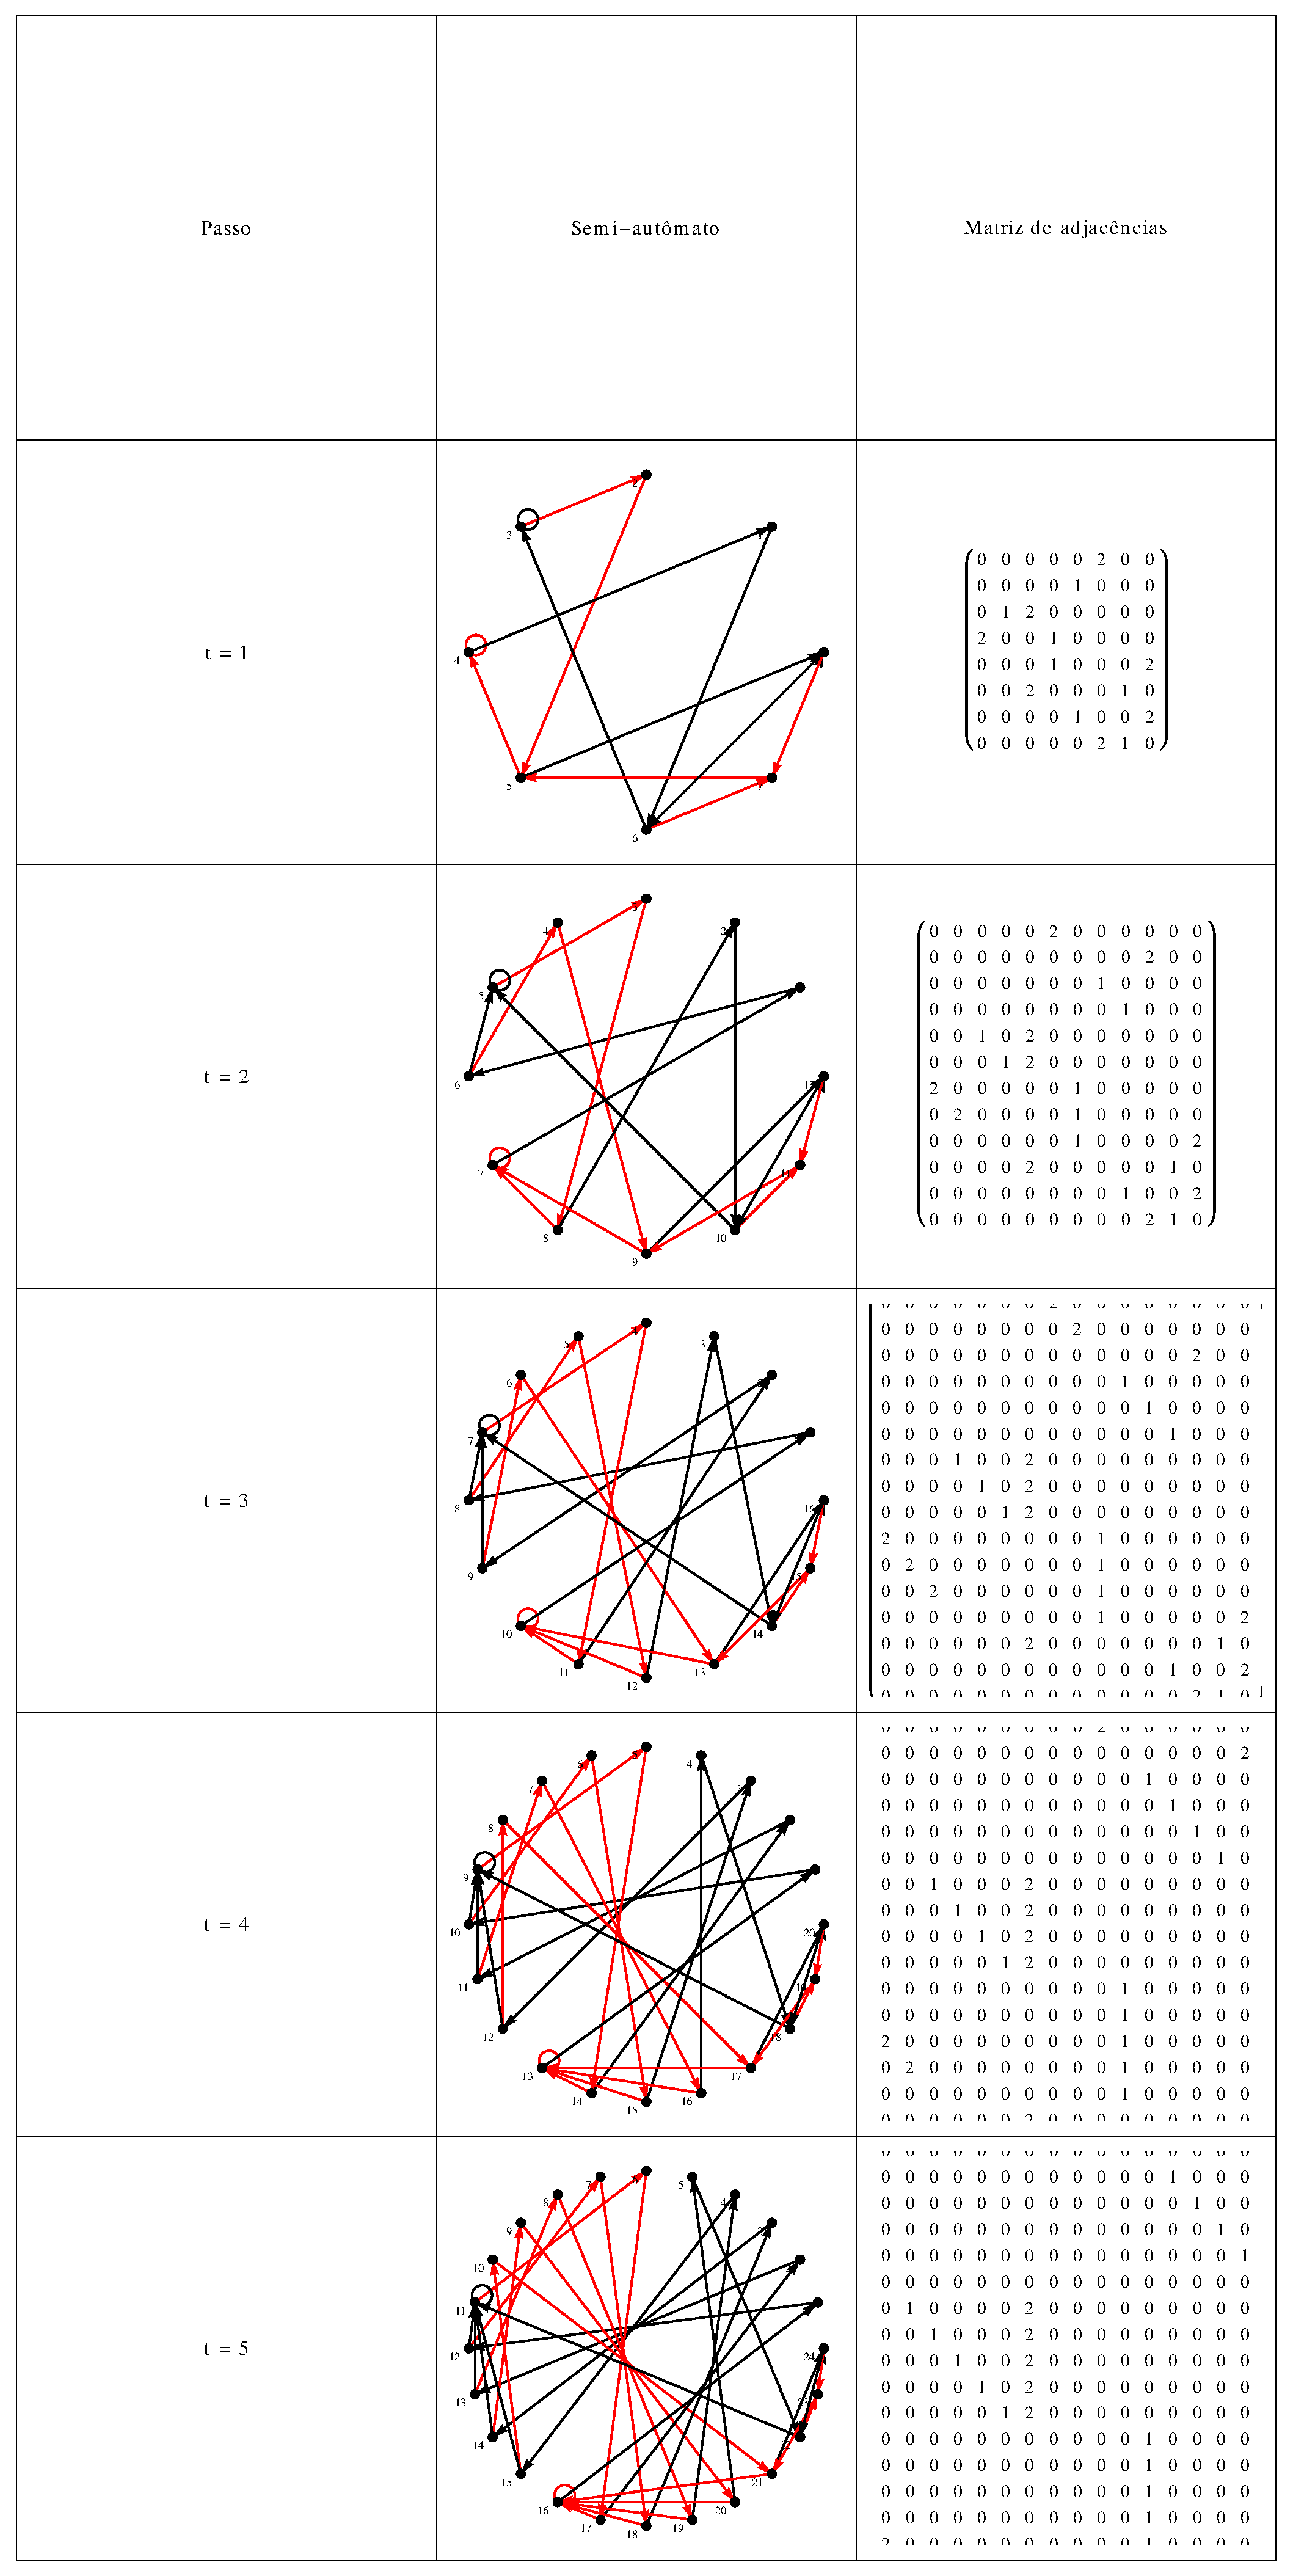
\includegraphics[scale=0.32]{img/mat/matr113.eps}
\caption{Regra 113.}
\label{tab:mr113}
\end{center}
\end{table}

\begin{table}[H]
\begin{center}
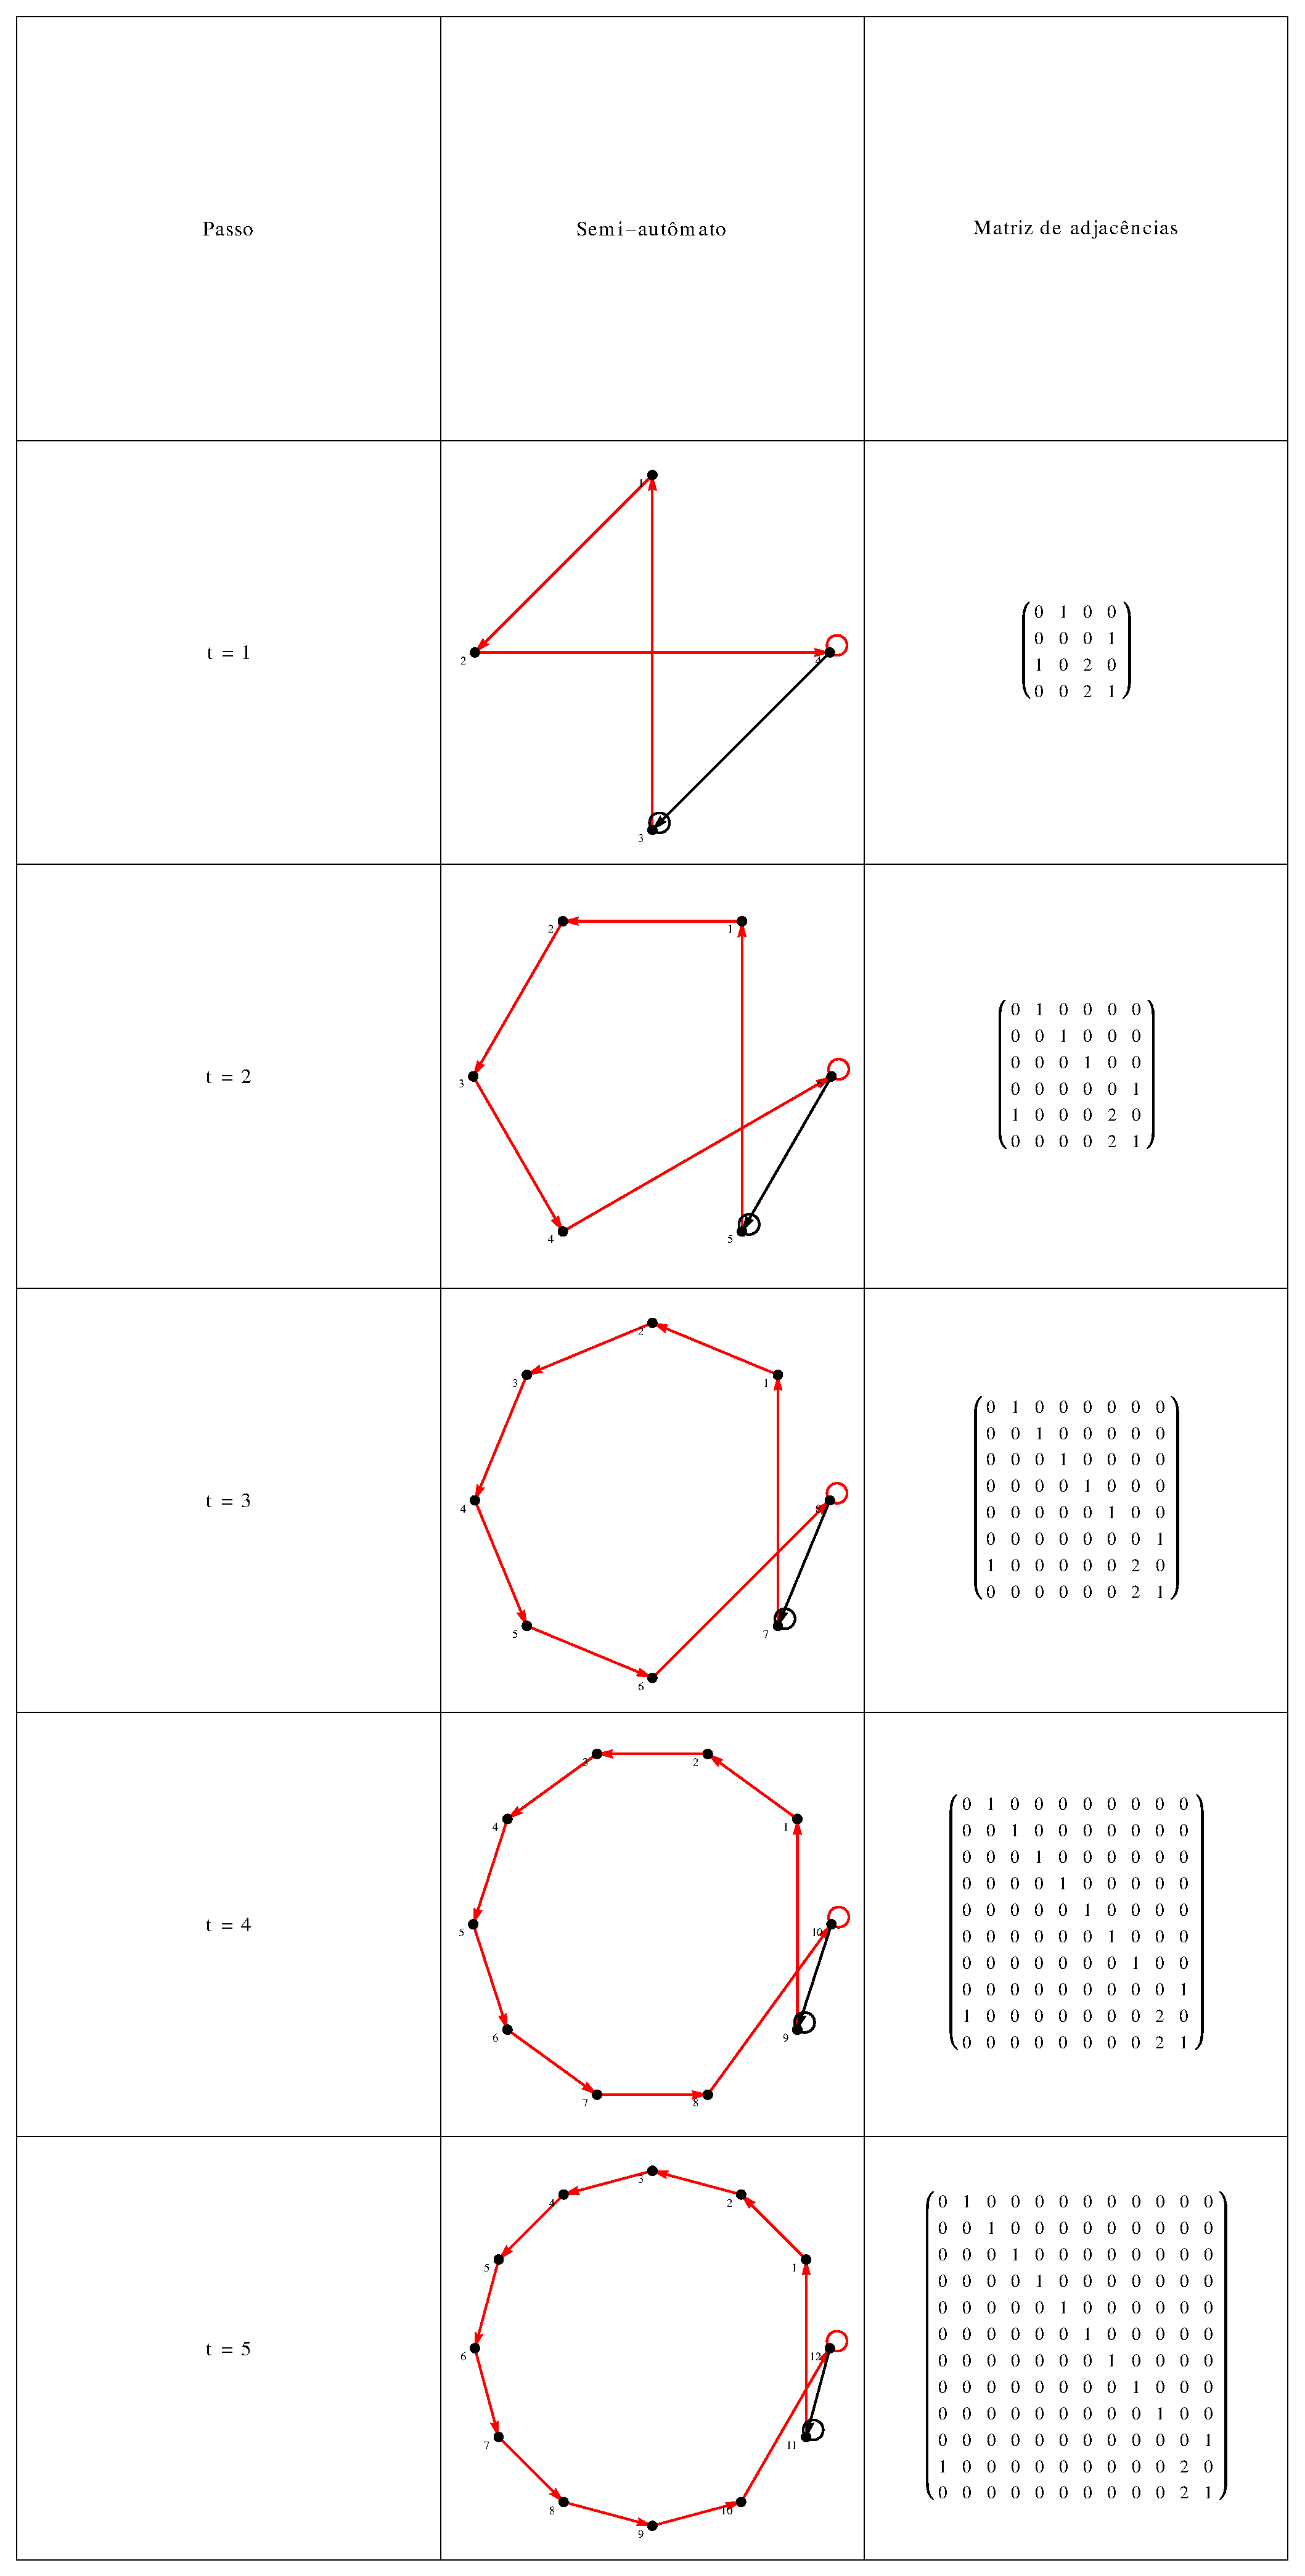
\includegraphics[scale=0.32]{img/mat/matr128.eps}
\caption{Regra 128.}
\label{tab:mr128}
\end{center}
\end{table}

\begin{table}[H]
\begin{center}
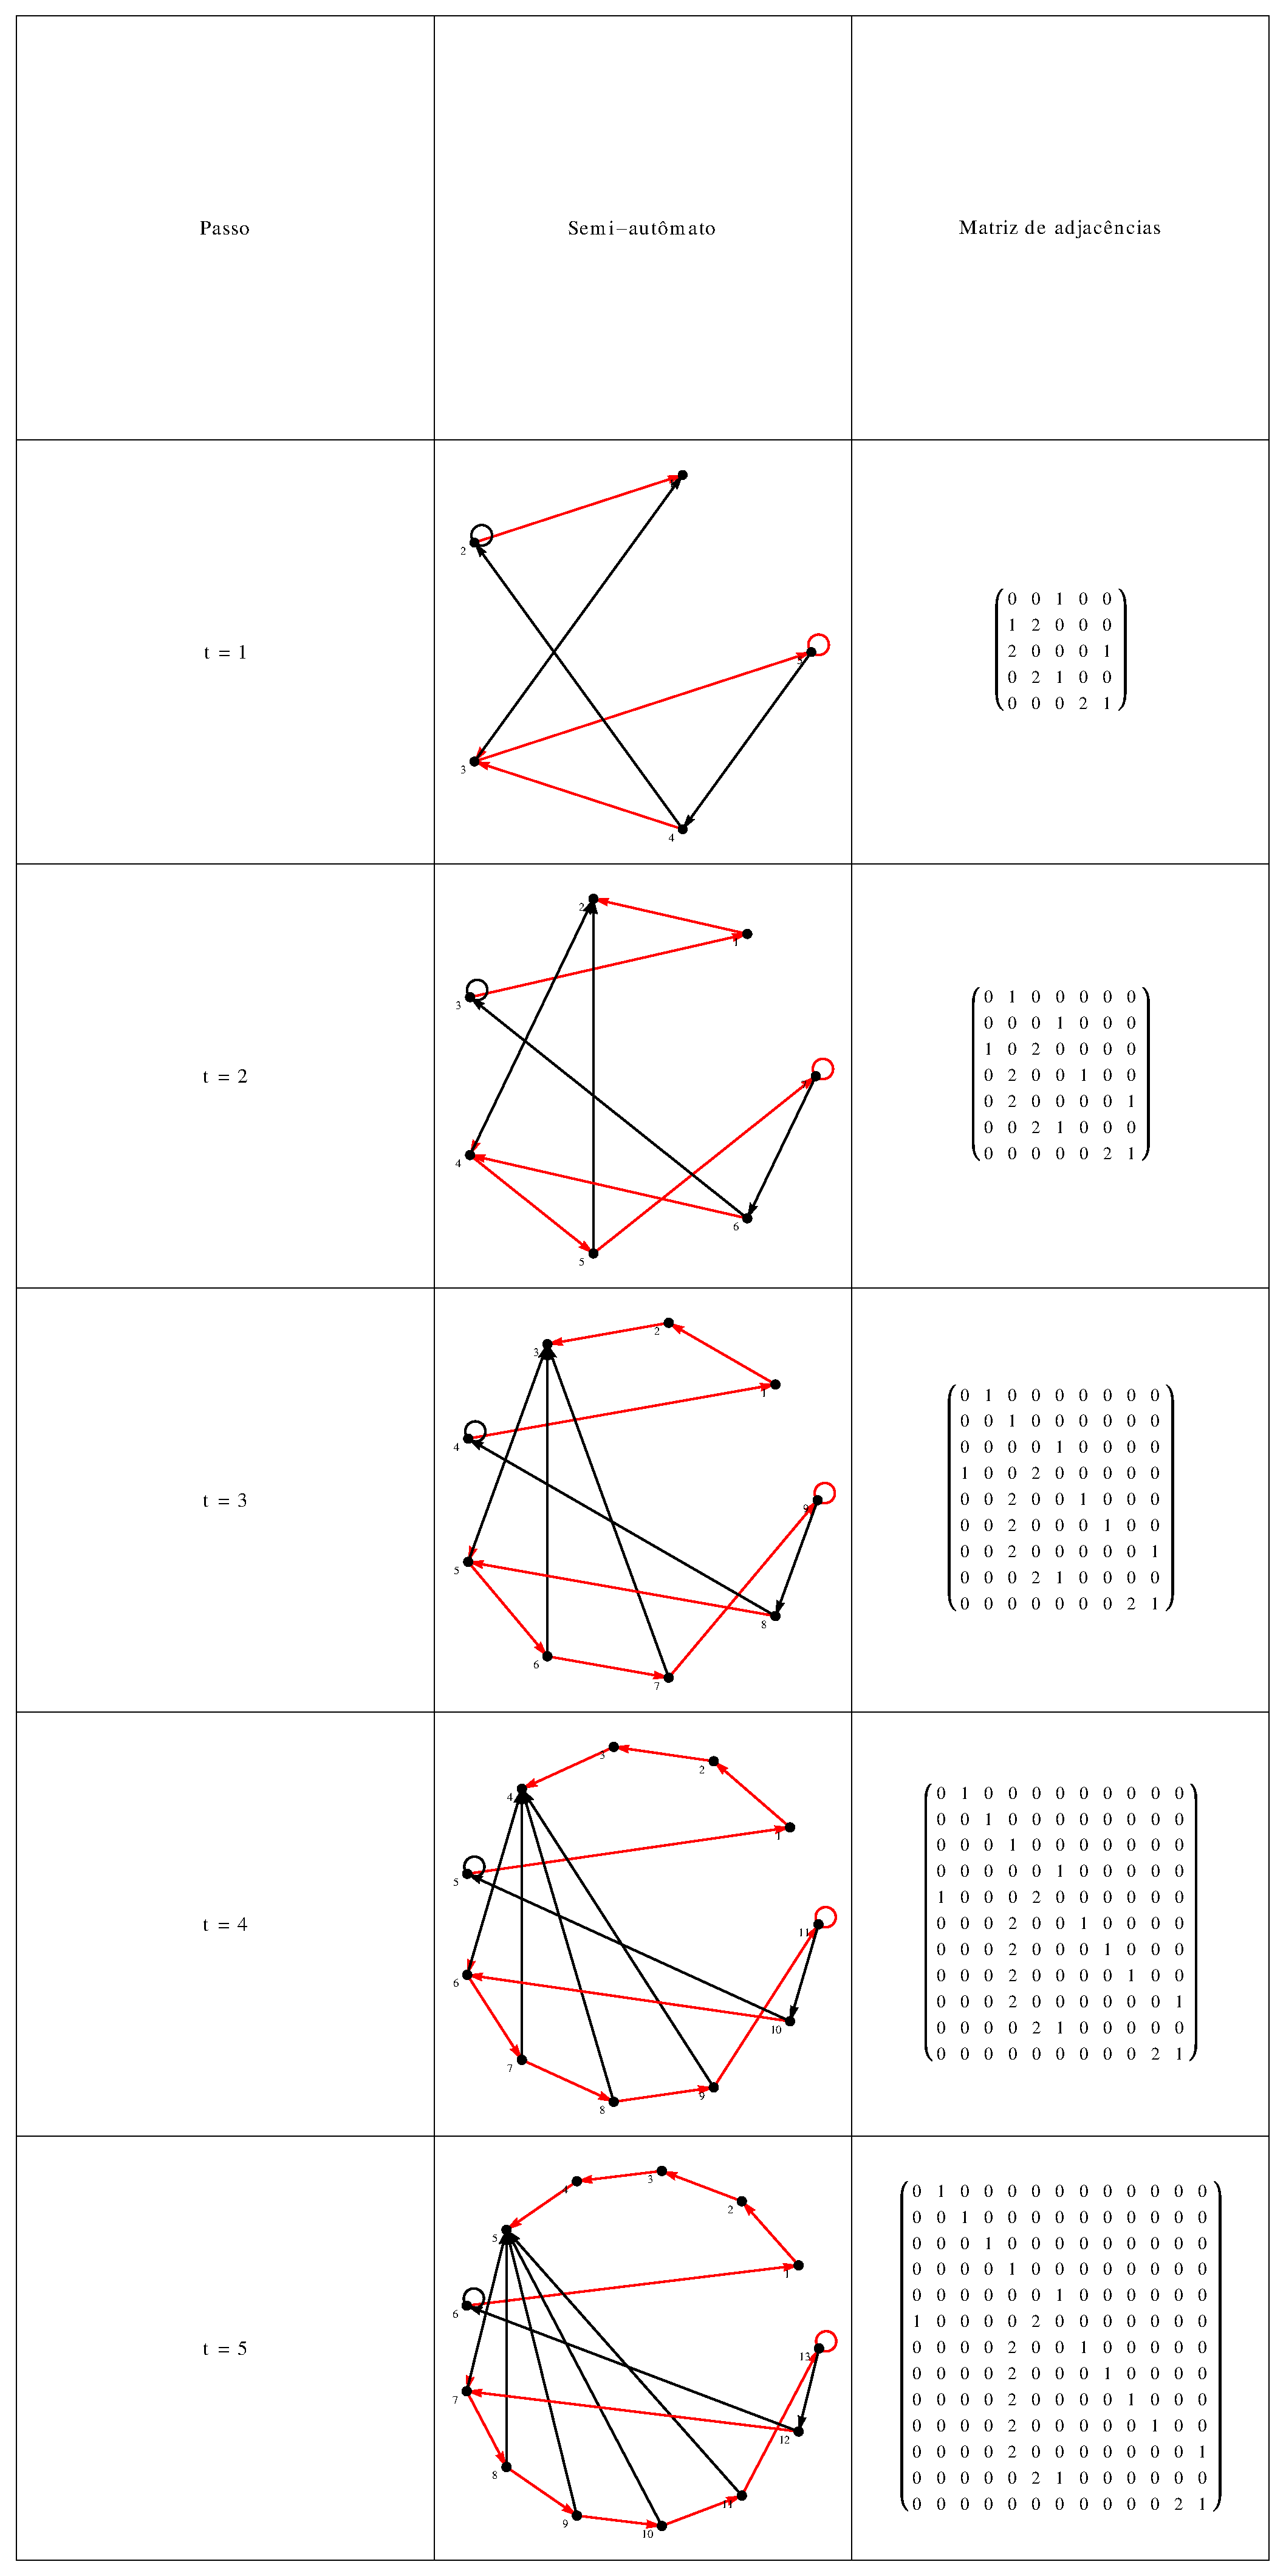
\includegraphics[scale=0.32]{img/mat/matr132.eps}
\caption{Regra 132.}
\label{tab:mr132}
\end{center}
\end{table}

\begin{table}[H]
\begin{center}
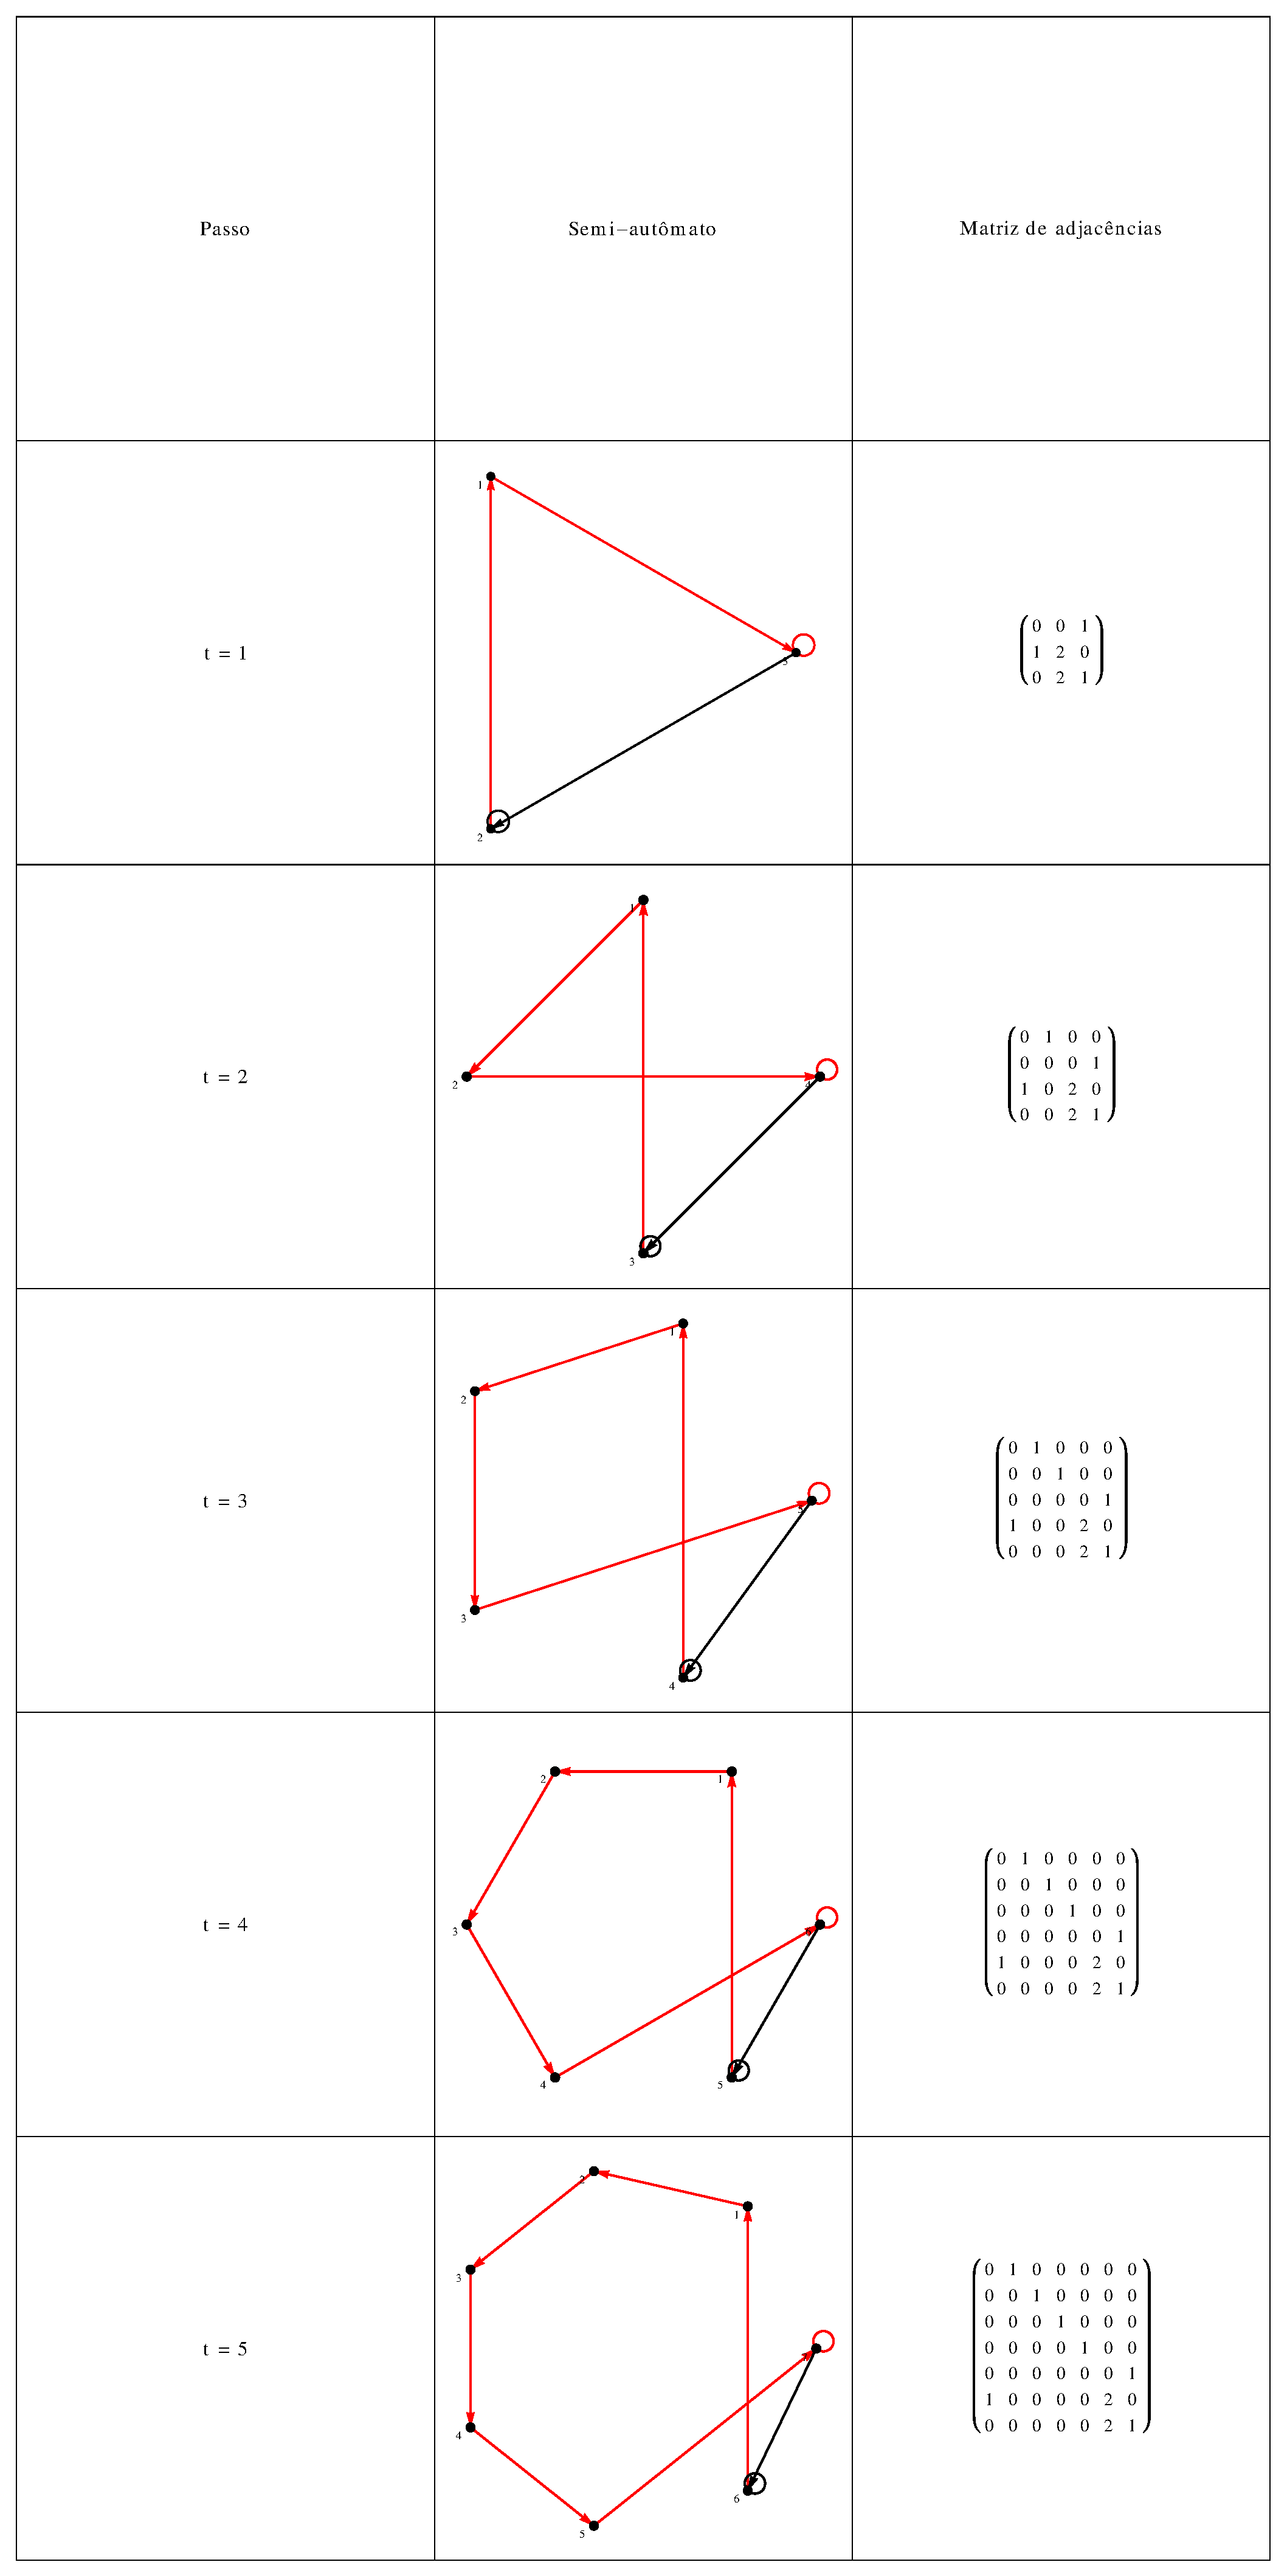
\includegraphics[scale=0.32]{img/mat/matr136.eps}
\caption{Regra 136.}
\label{tab:mr136}
\end{center}
\end{table}

\begin{table}[H]
\begin{center}
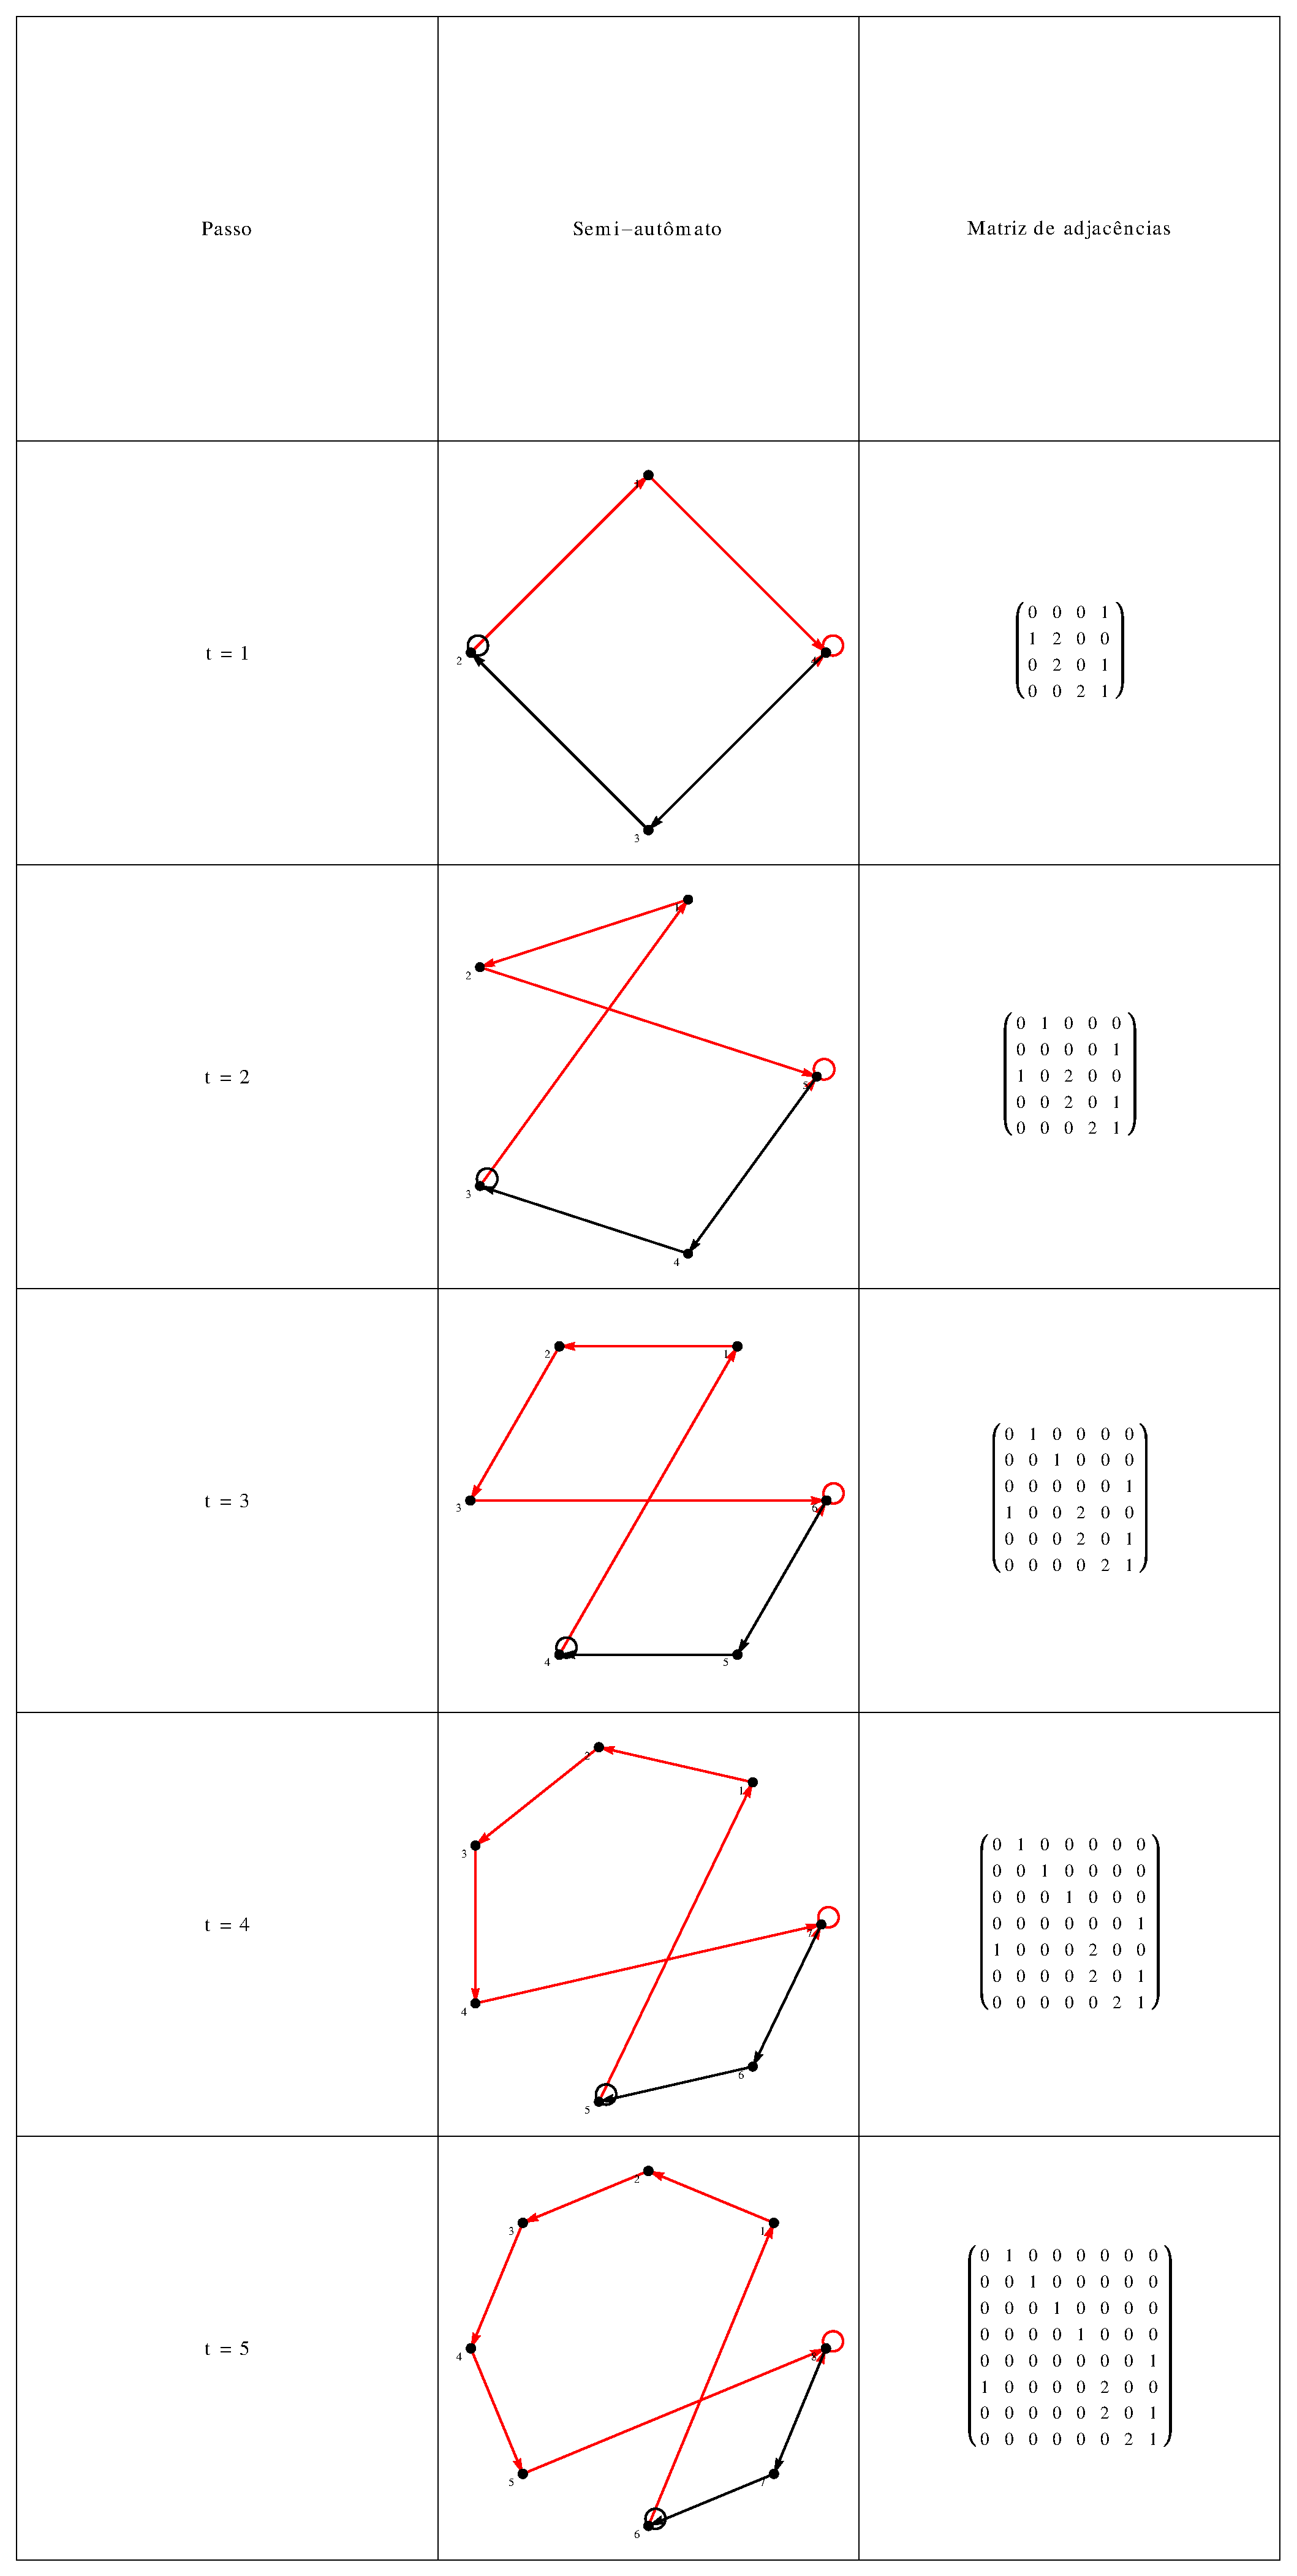
\includegraphics[scale=0.32]{img/mat/matr140.eps}
\caption{Regra 140.}
\label{tab:mr140}
\end{center}
\end{table}

\begin{table}[H]
\begin{center}
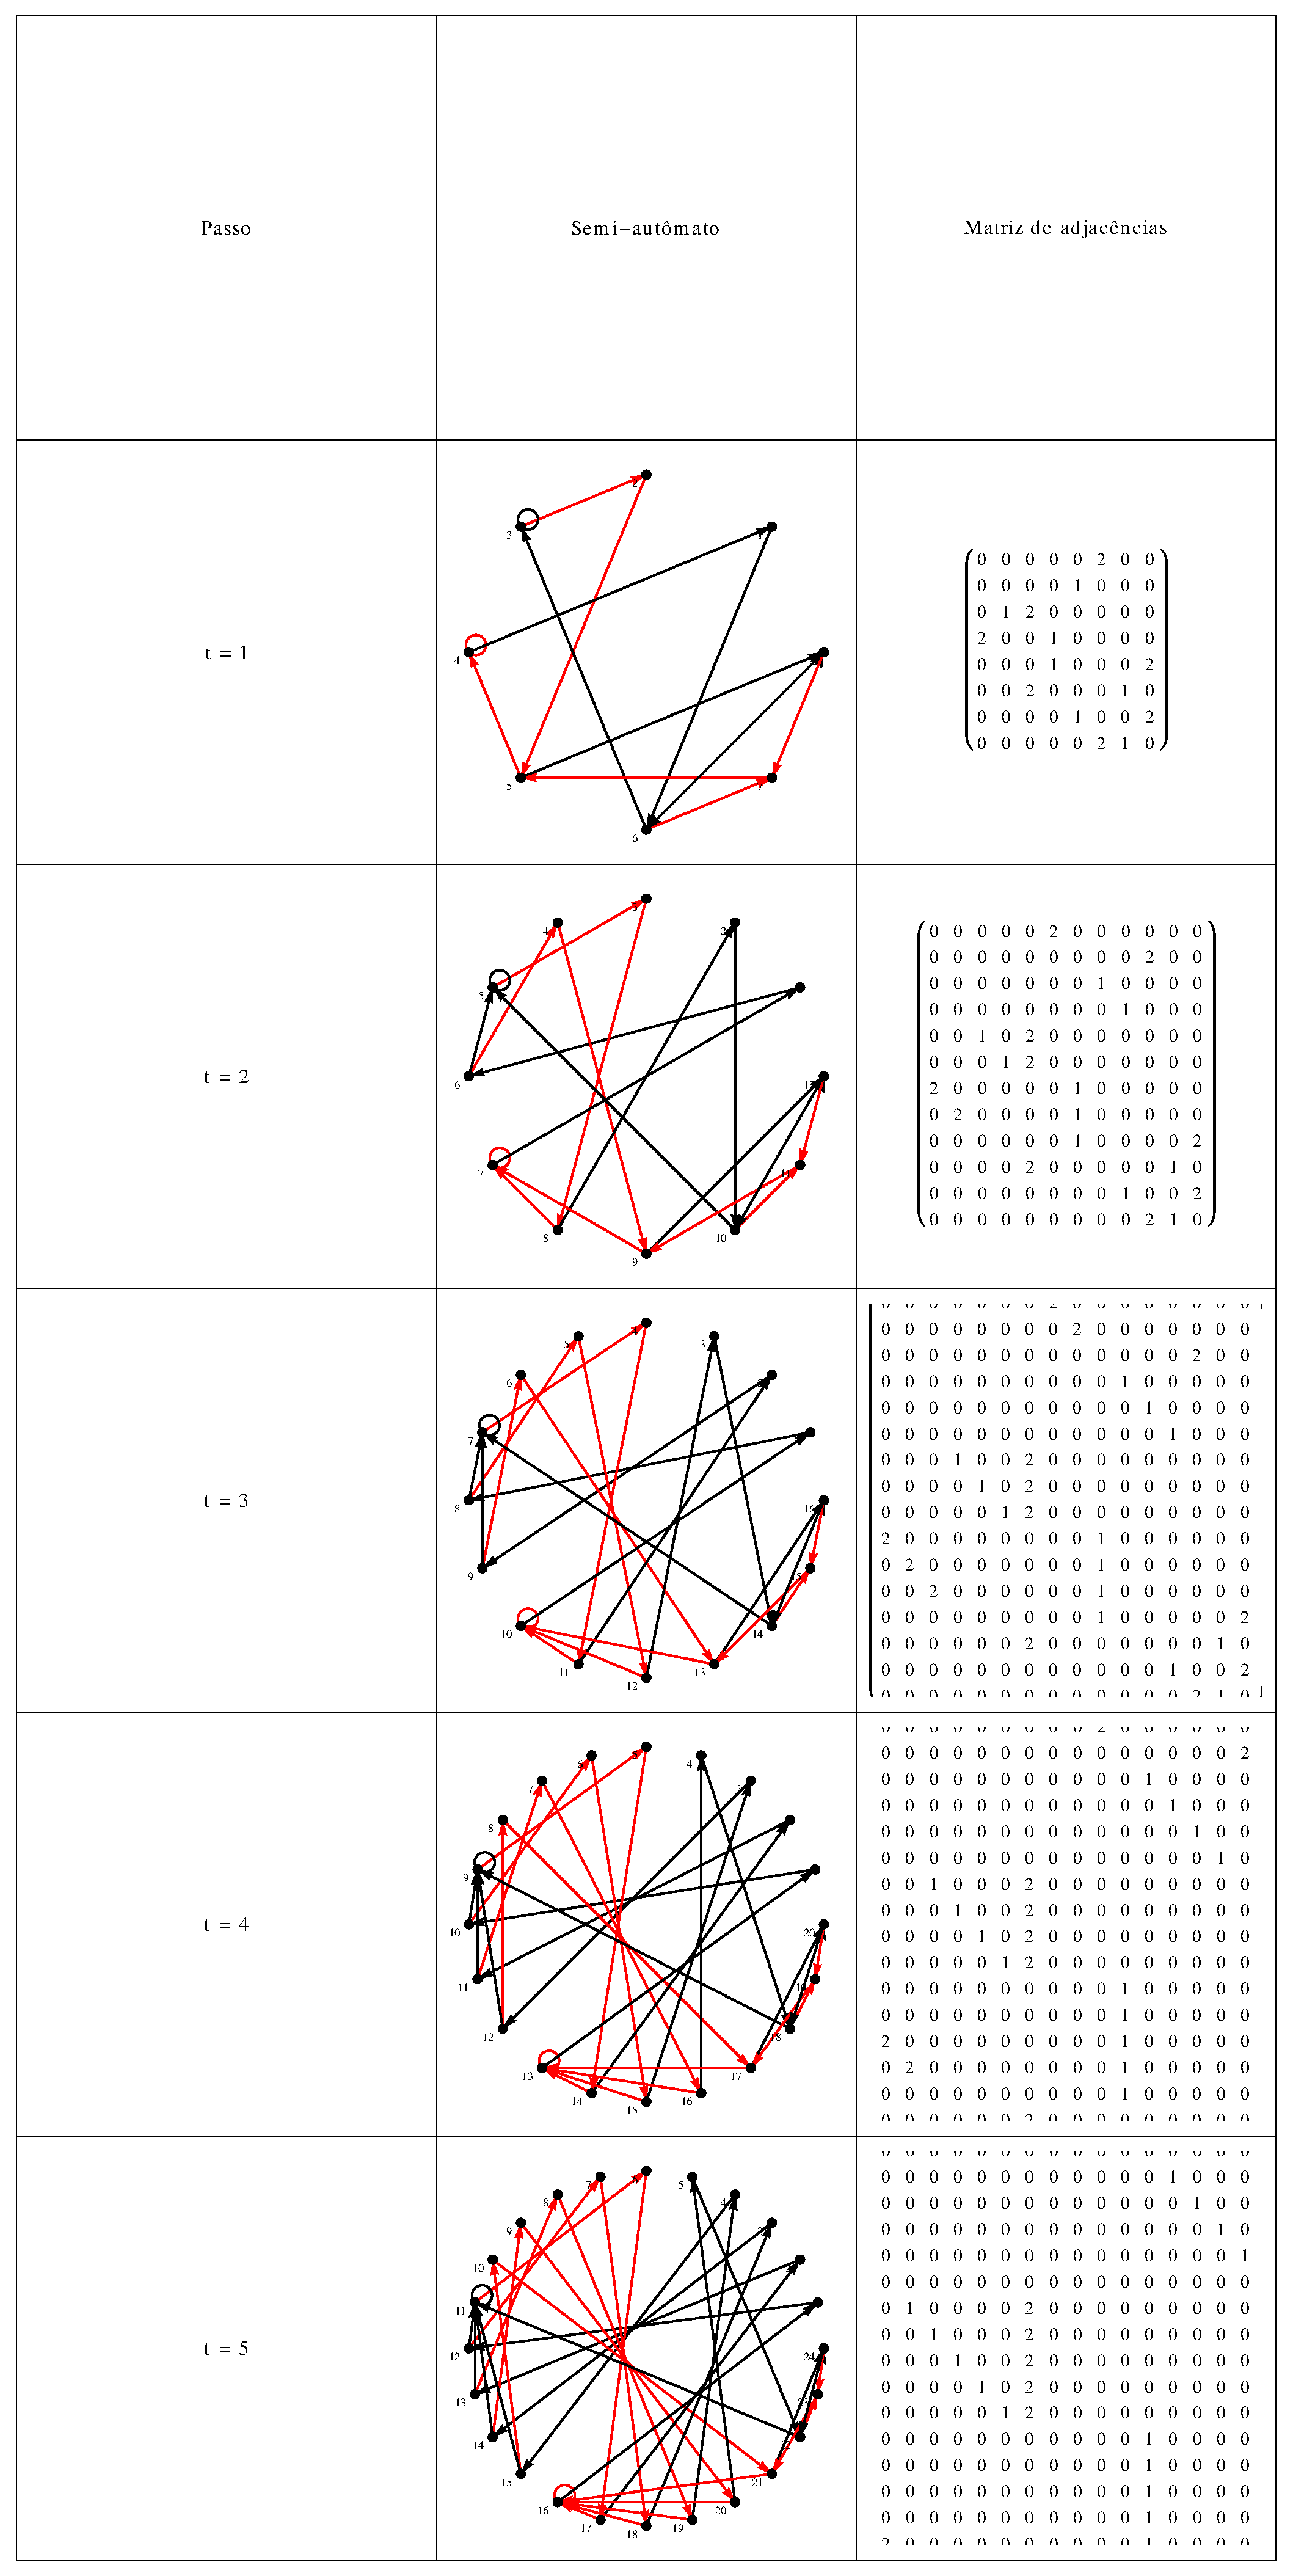
\includegraphics[scale=0.32]{img/mat/matr142.eps}
\caption{Regra 142.}
\label{tab:mr142}
\end{center}
\end{table}

\begin{table}[H]
\begin{center}
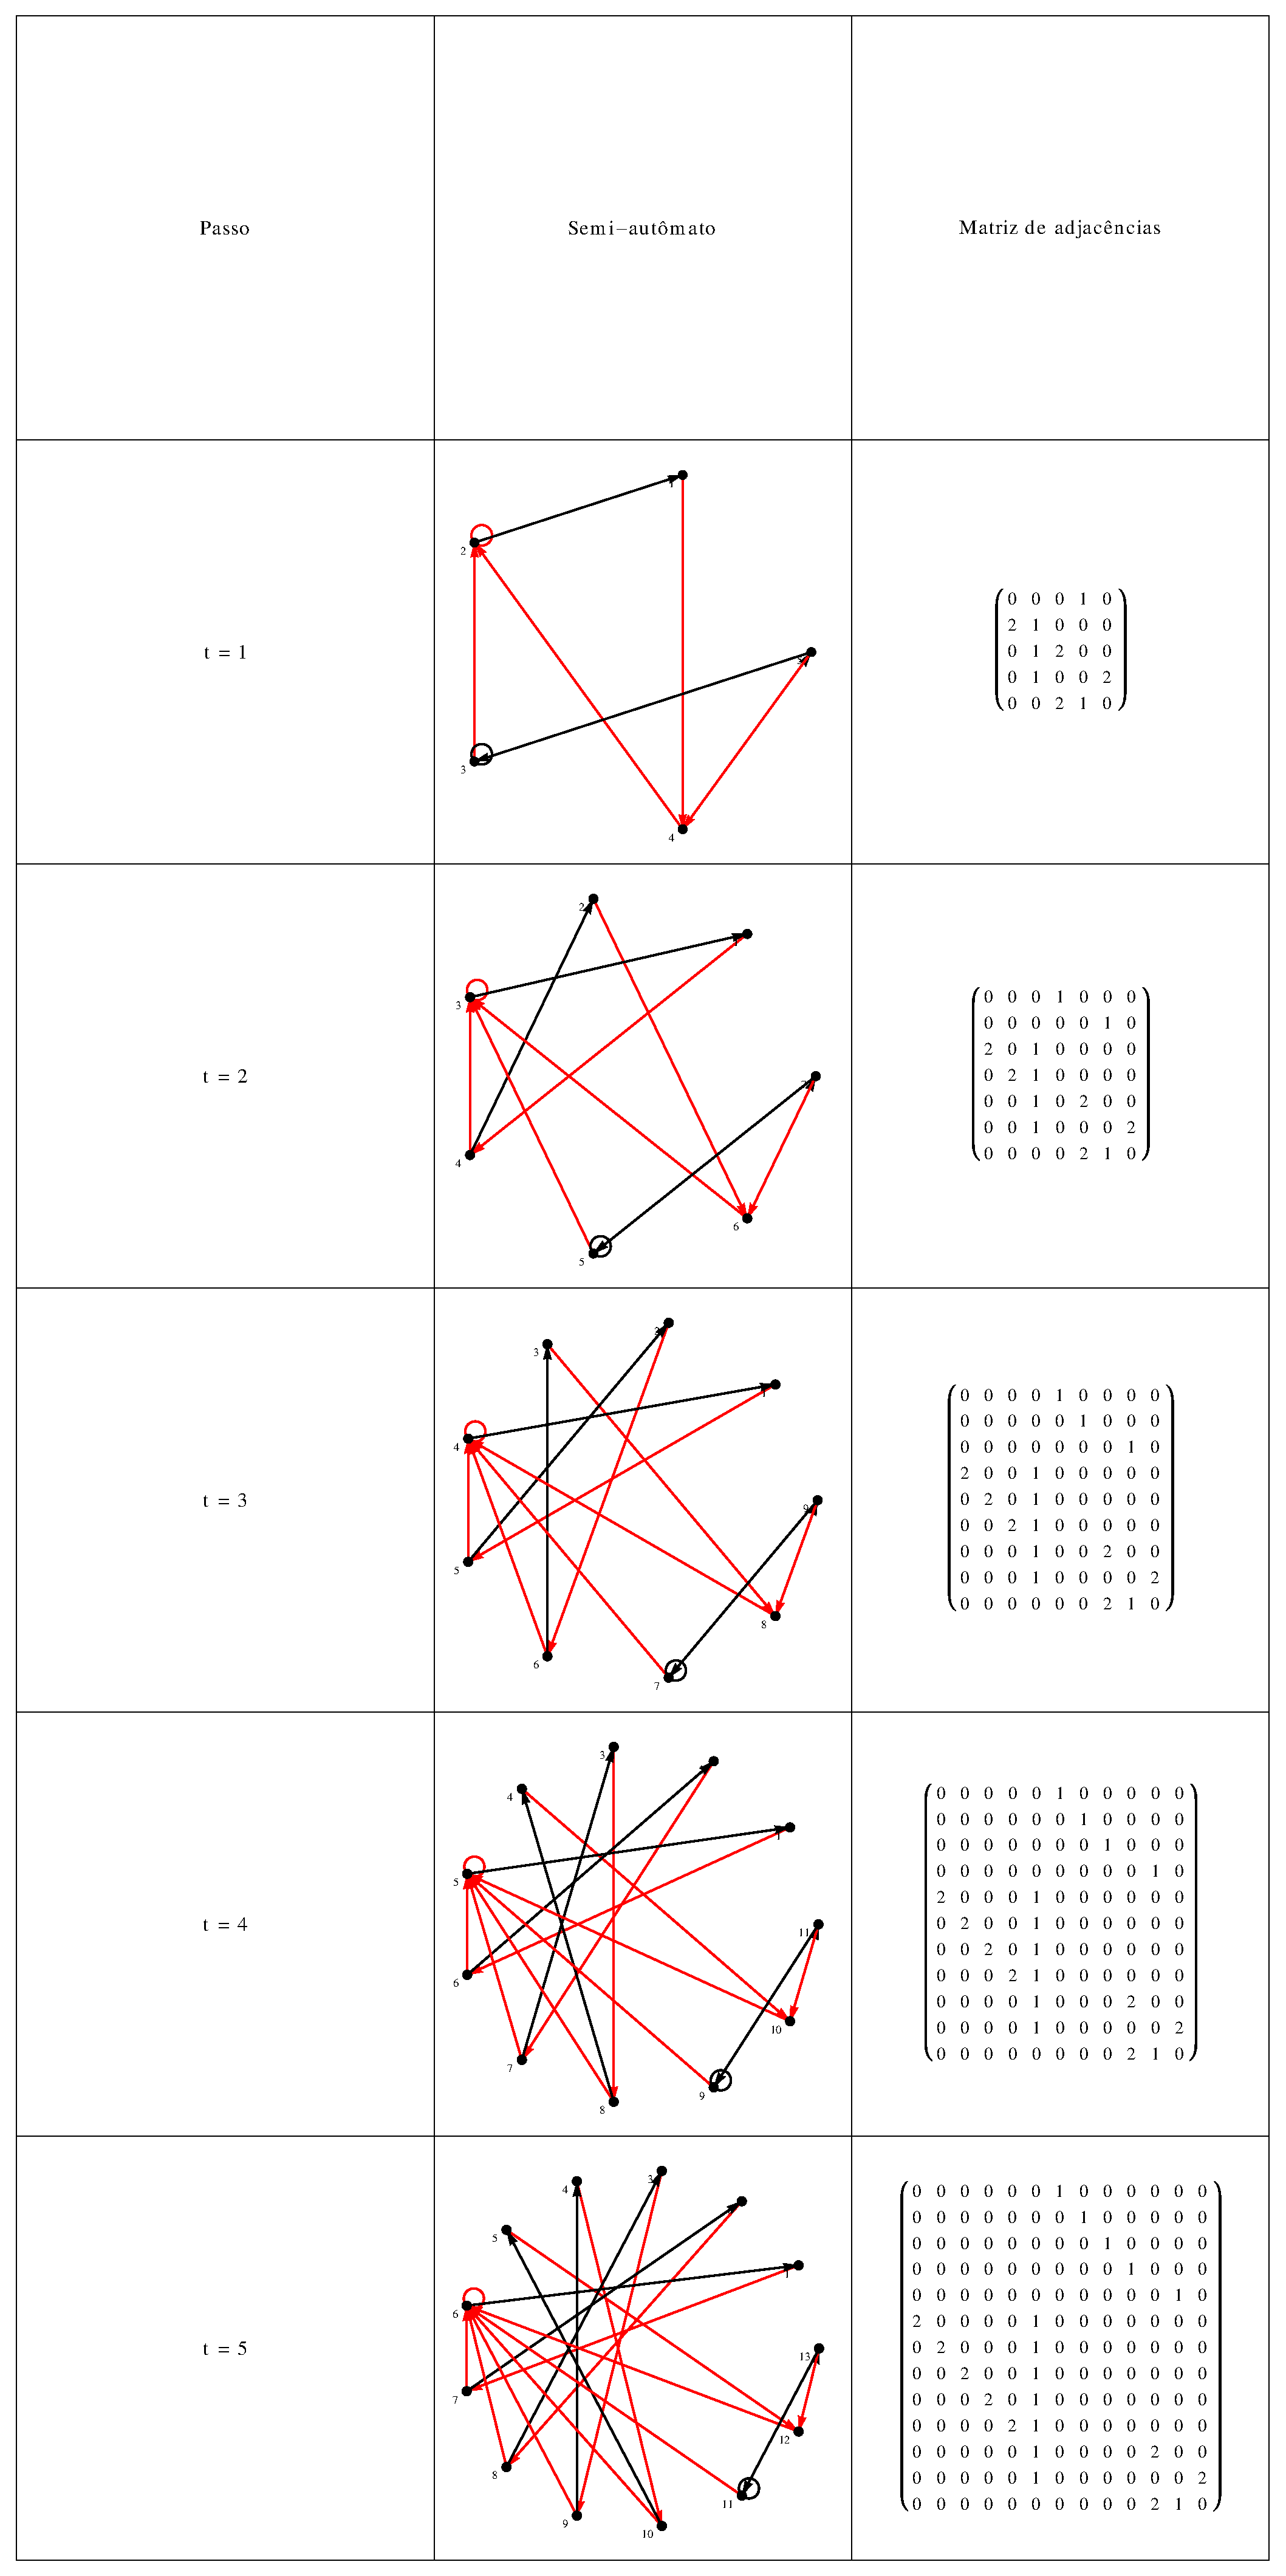
\includegraphics[scale=0.32]{img/mat/matr162.eps}
\caption{Regra 162.}
\label{tab:mr162}
\end{center}
\end{table}

\begin{table}[H]
\begin{center}
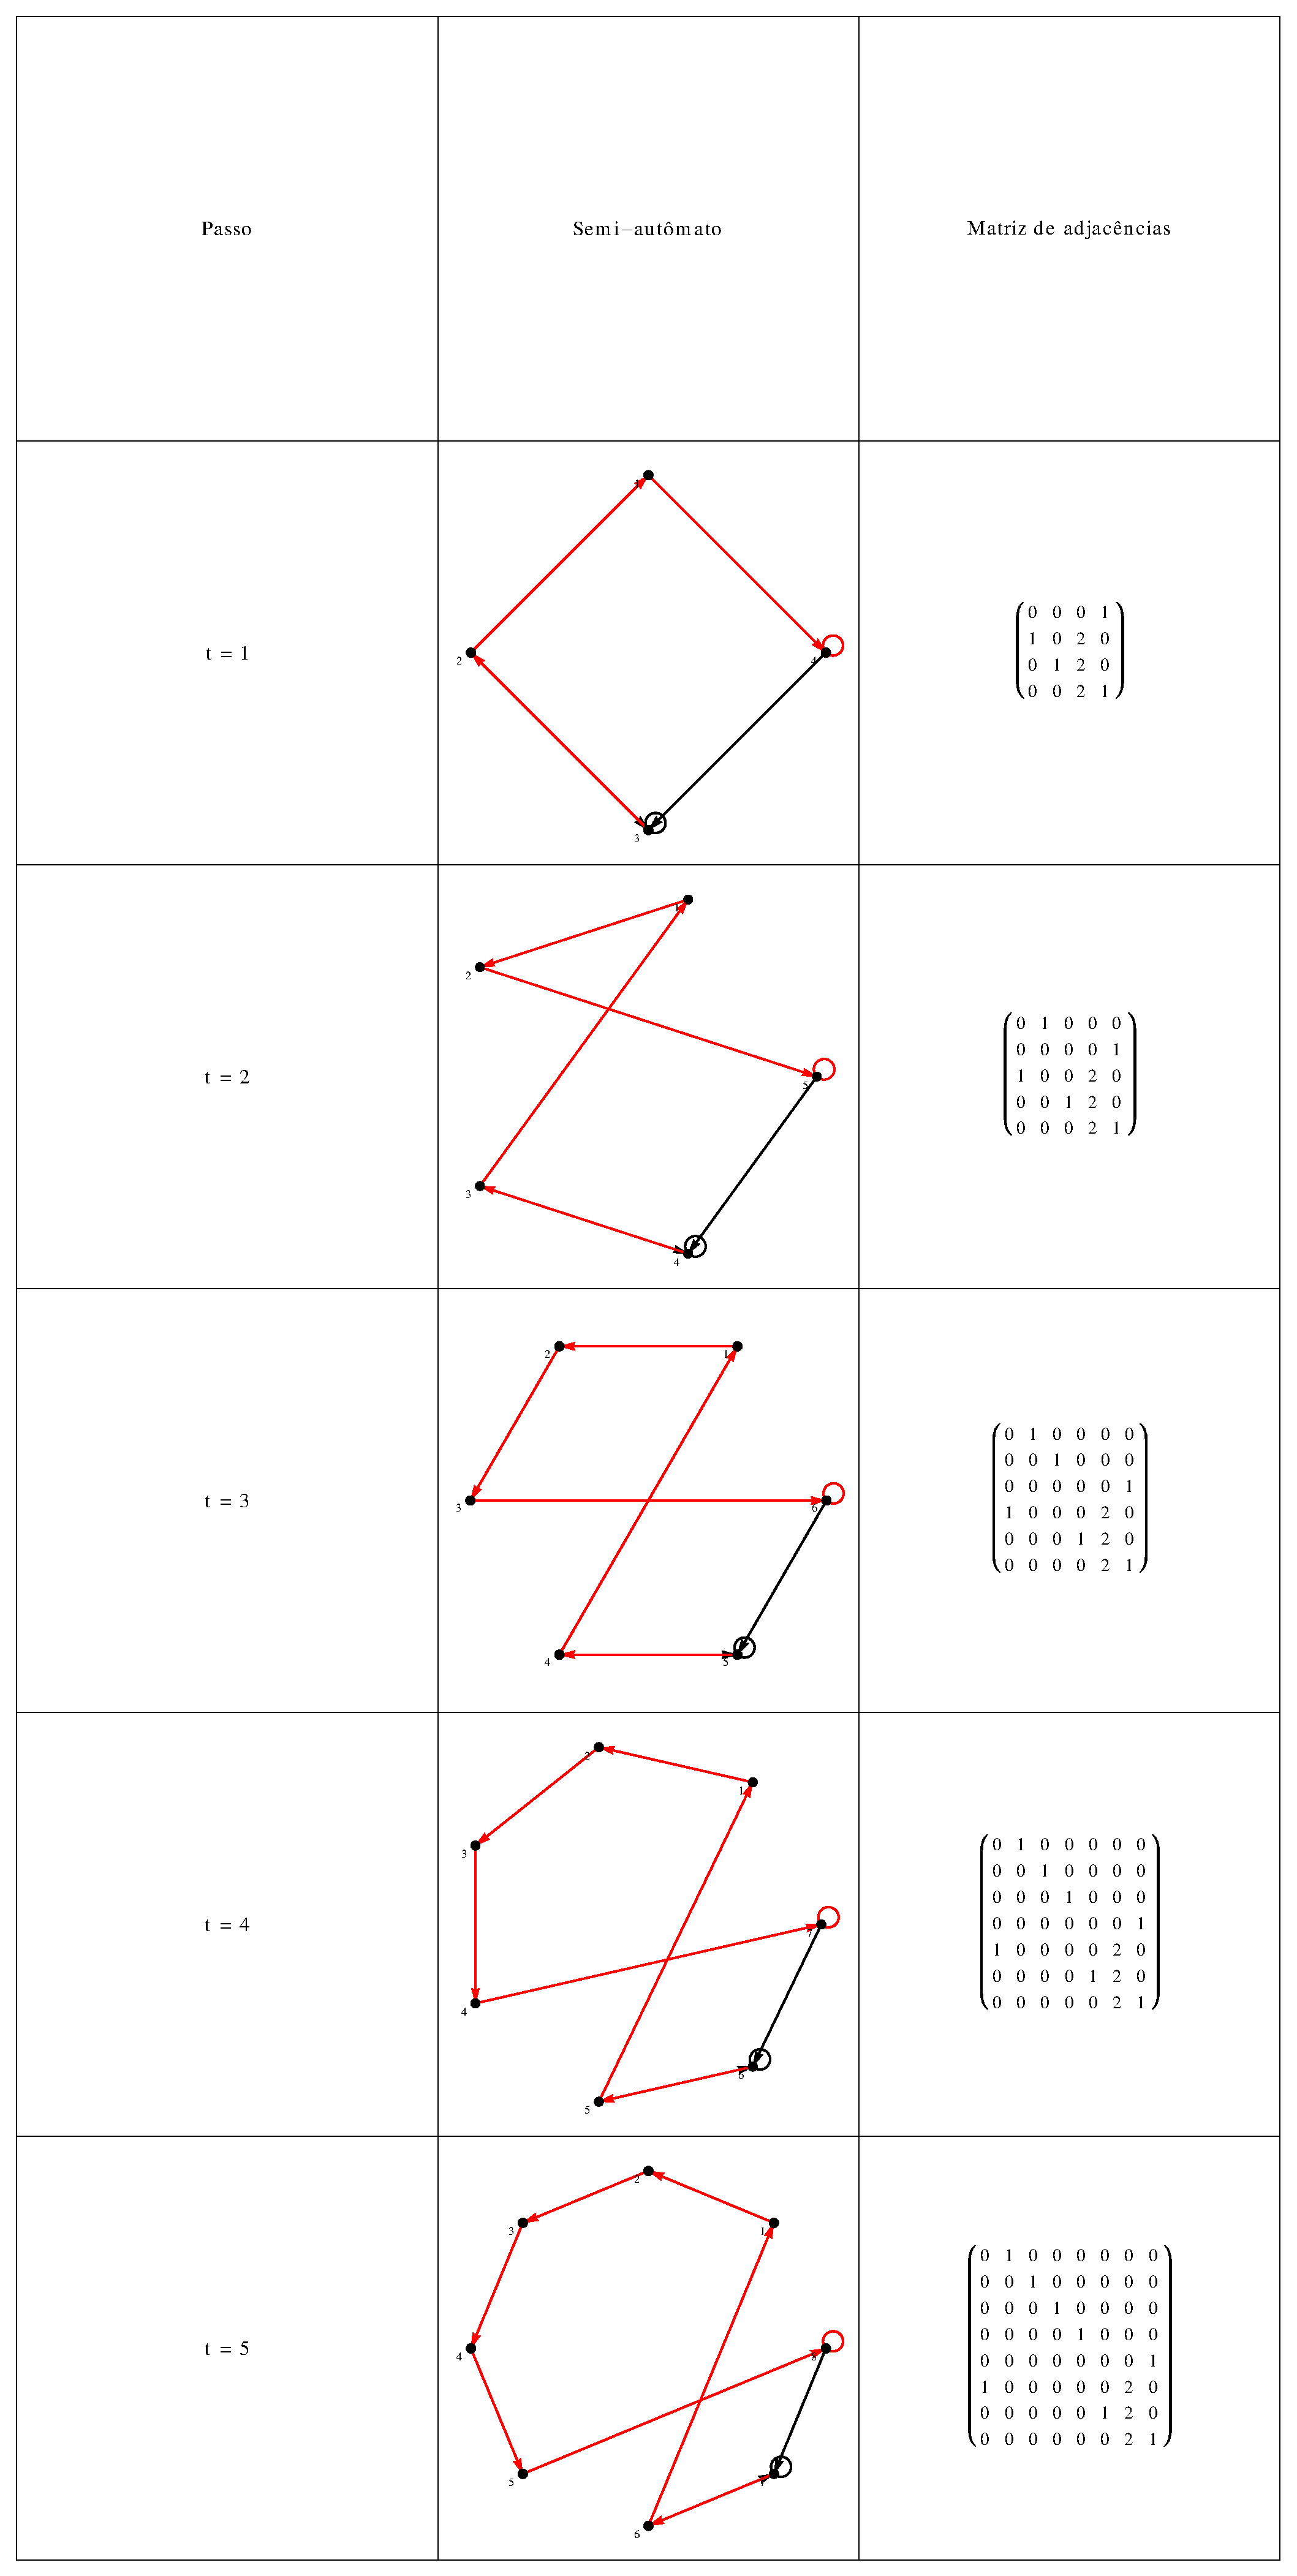
\includegraphics[scale=0.32]{img/mat/matr168.eps}
\caption{Regra 168.}
\label{tab:mr168}
\end{center}
\end{table}

\begin{table}[H]
\begin{center}
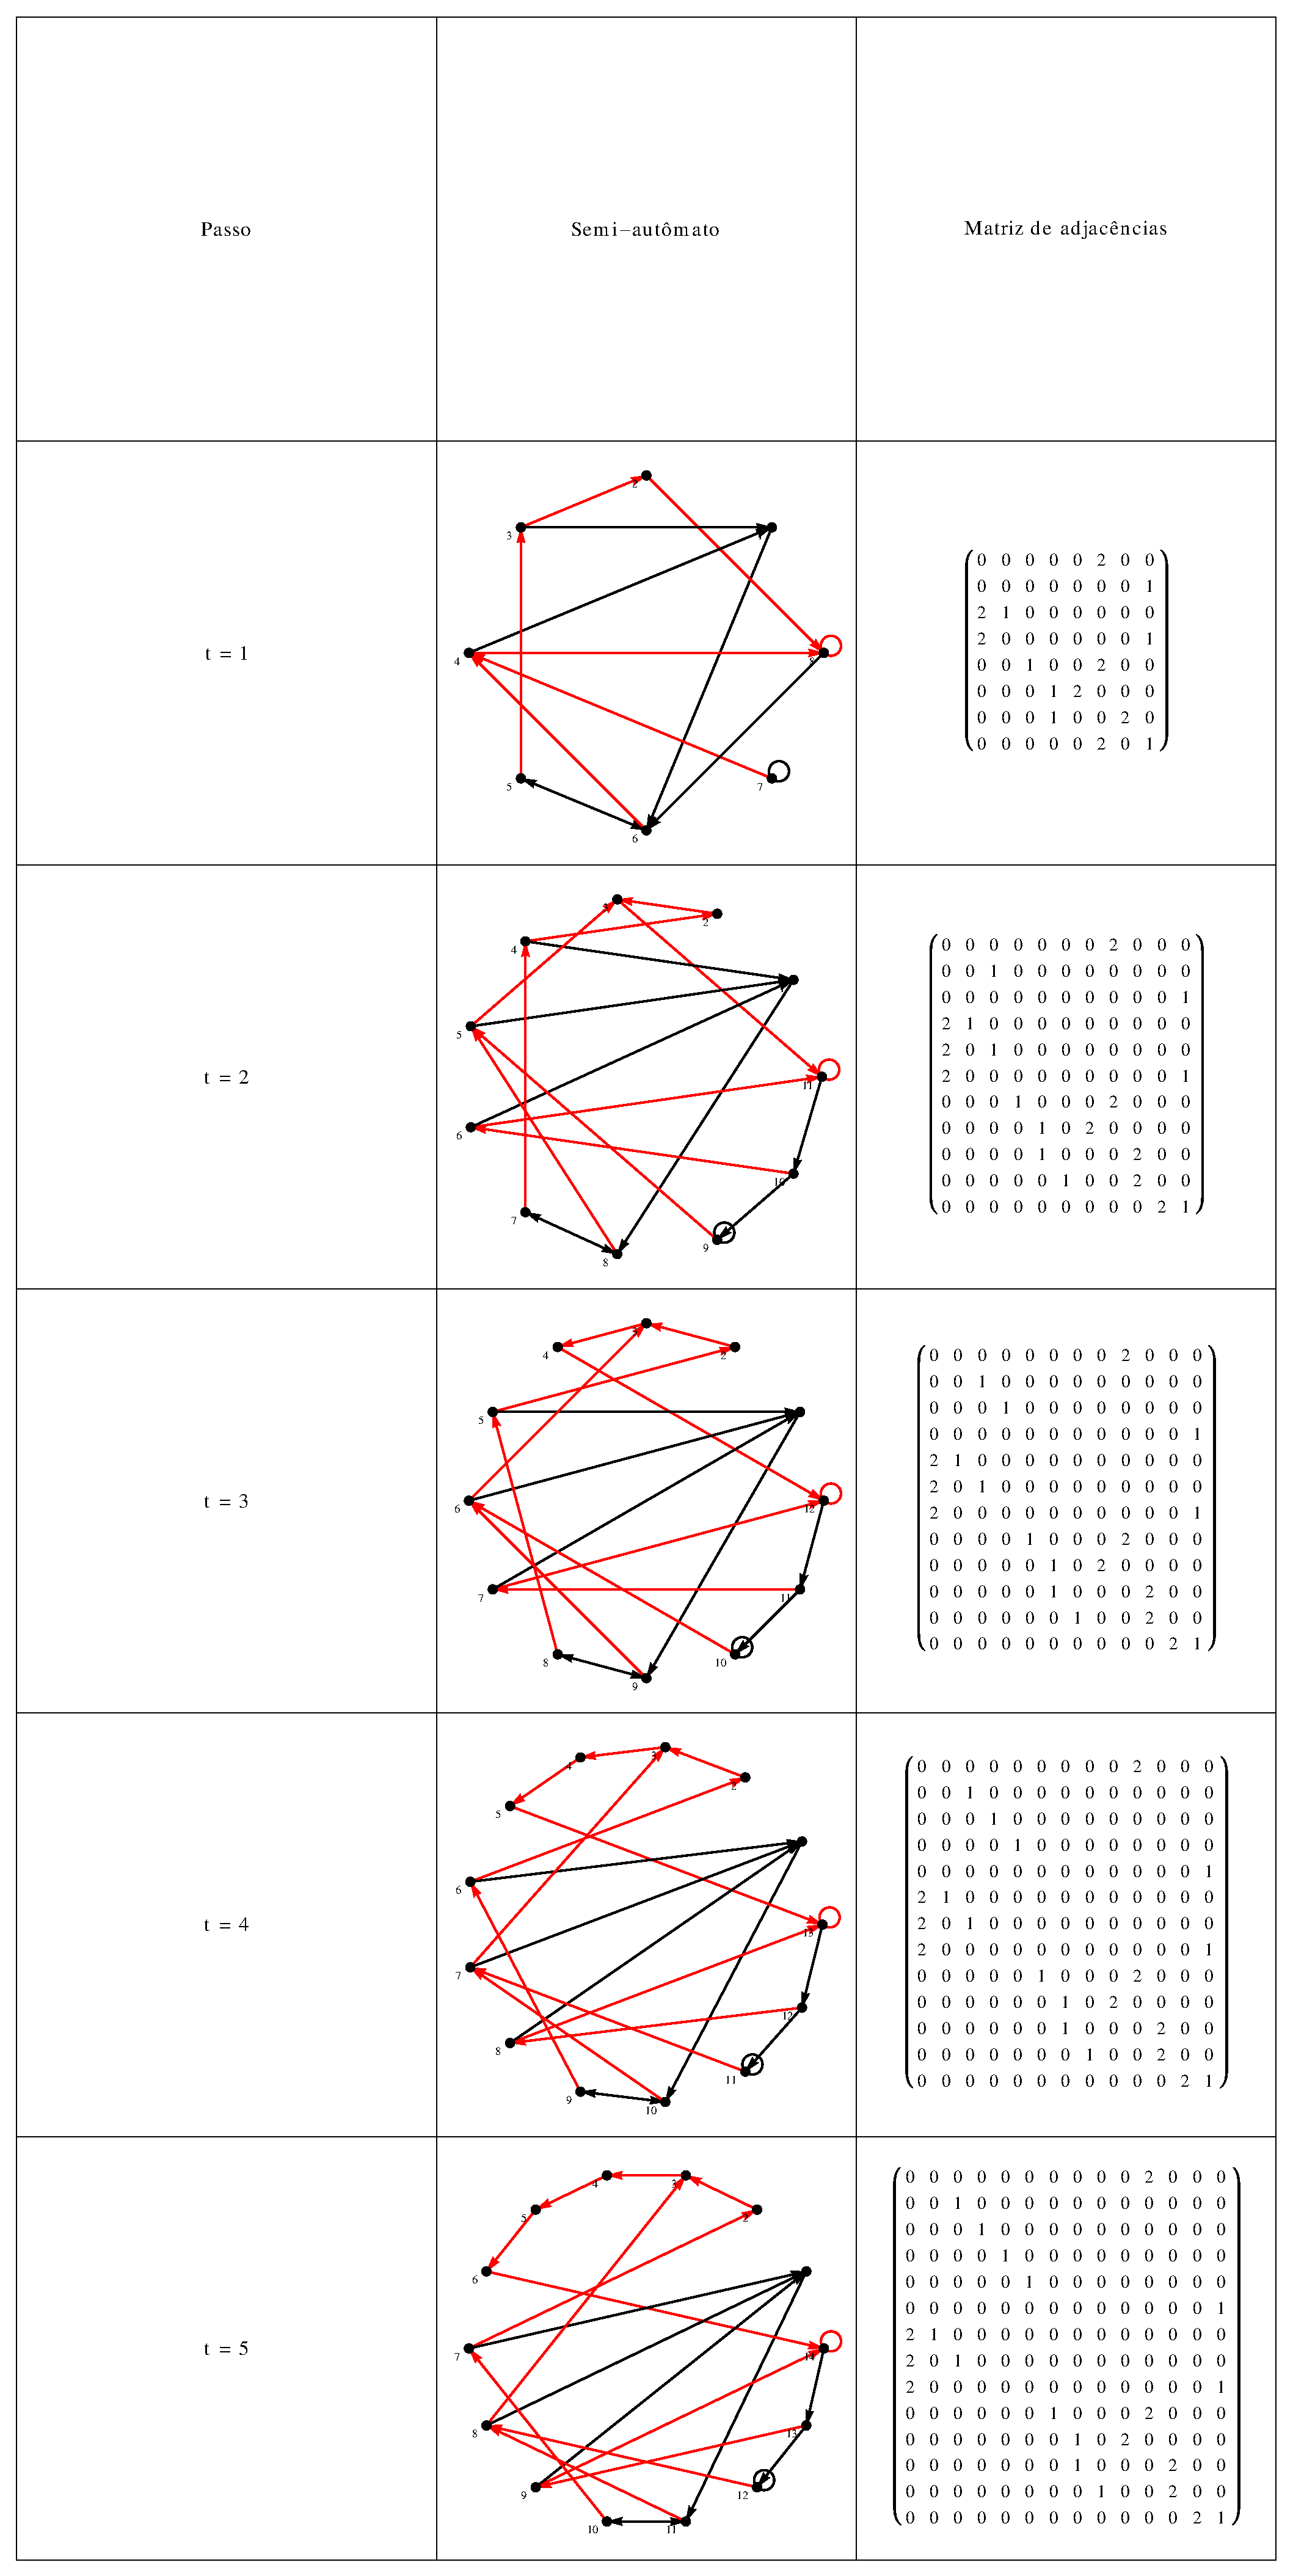
\includegraphics[scale=0.32]{img/mat/matr172.eps}
\caption{Regra 172.}
\label{tab:mr172}
\end{center}
\end{table}

\begin{table}[H]
\begin{center}
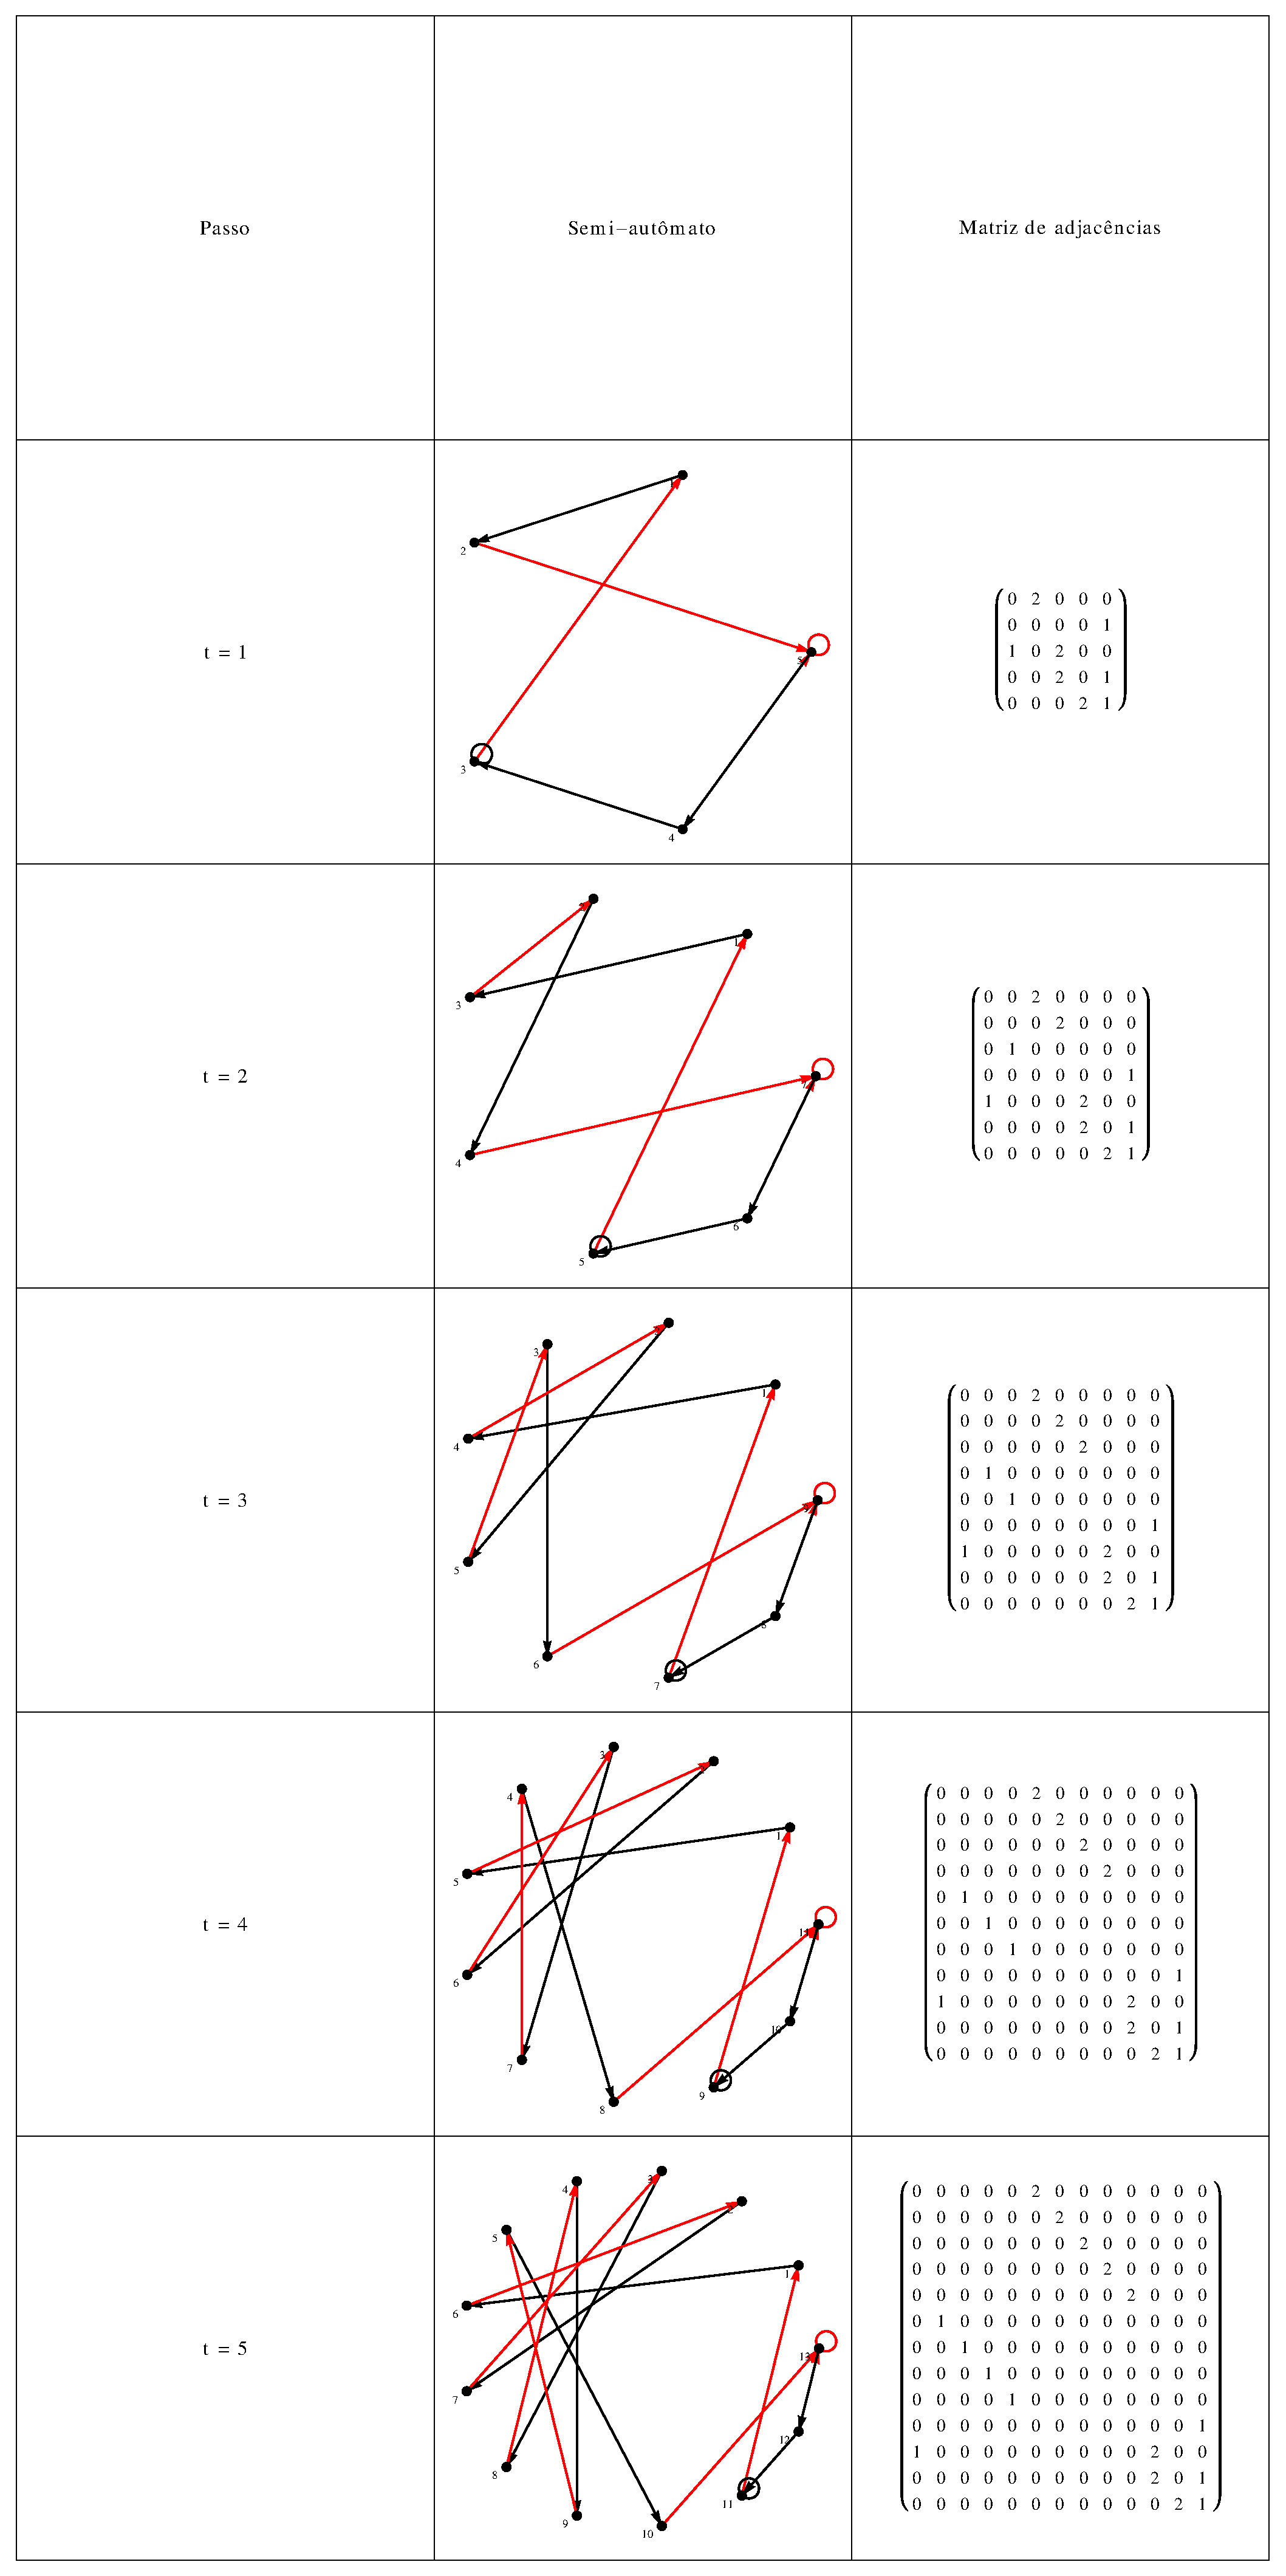
\includegraphics[scale=0.32]{img/mat/matr176.eps}
\caption{Regra 176.}
\label{tab:mr176}
\end{center}
\end{table}

\begin{table}[H]
\begin{center}
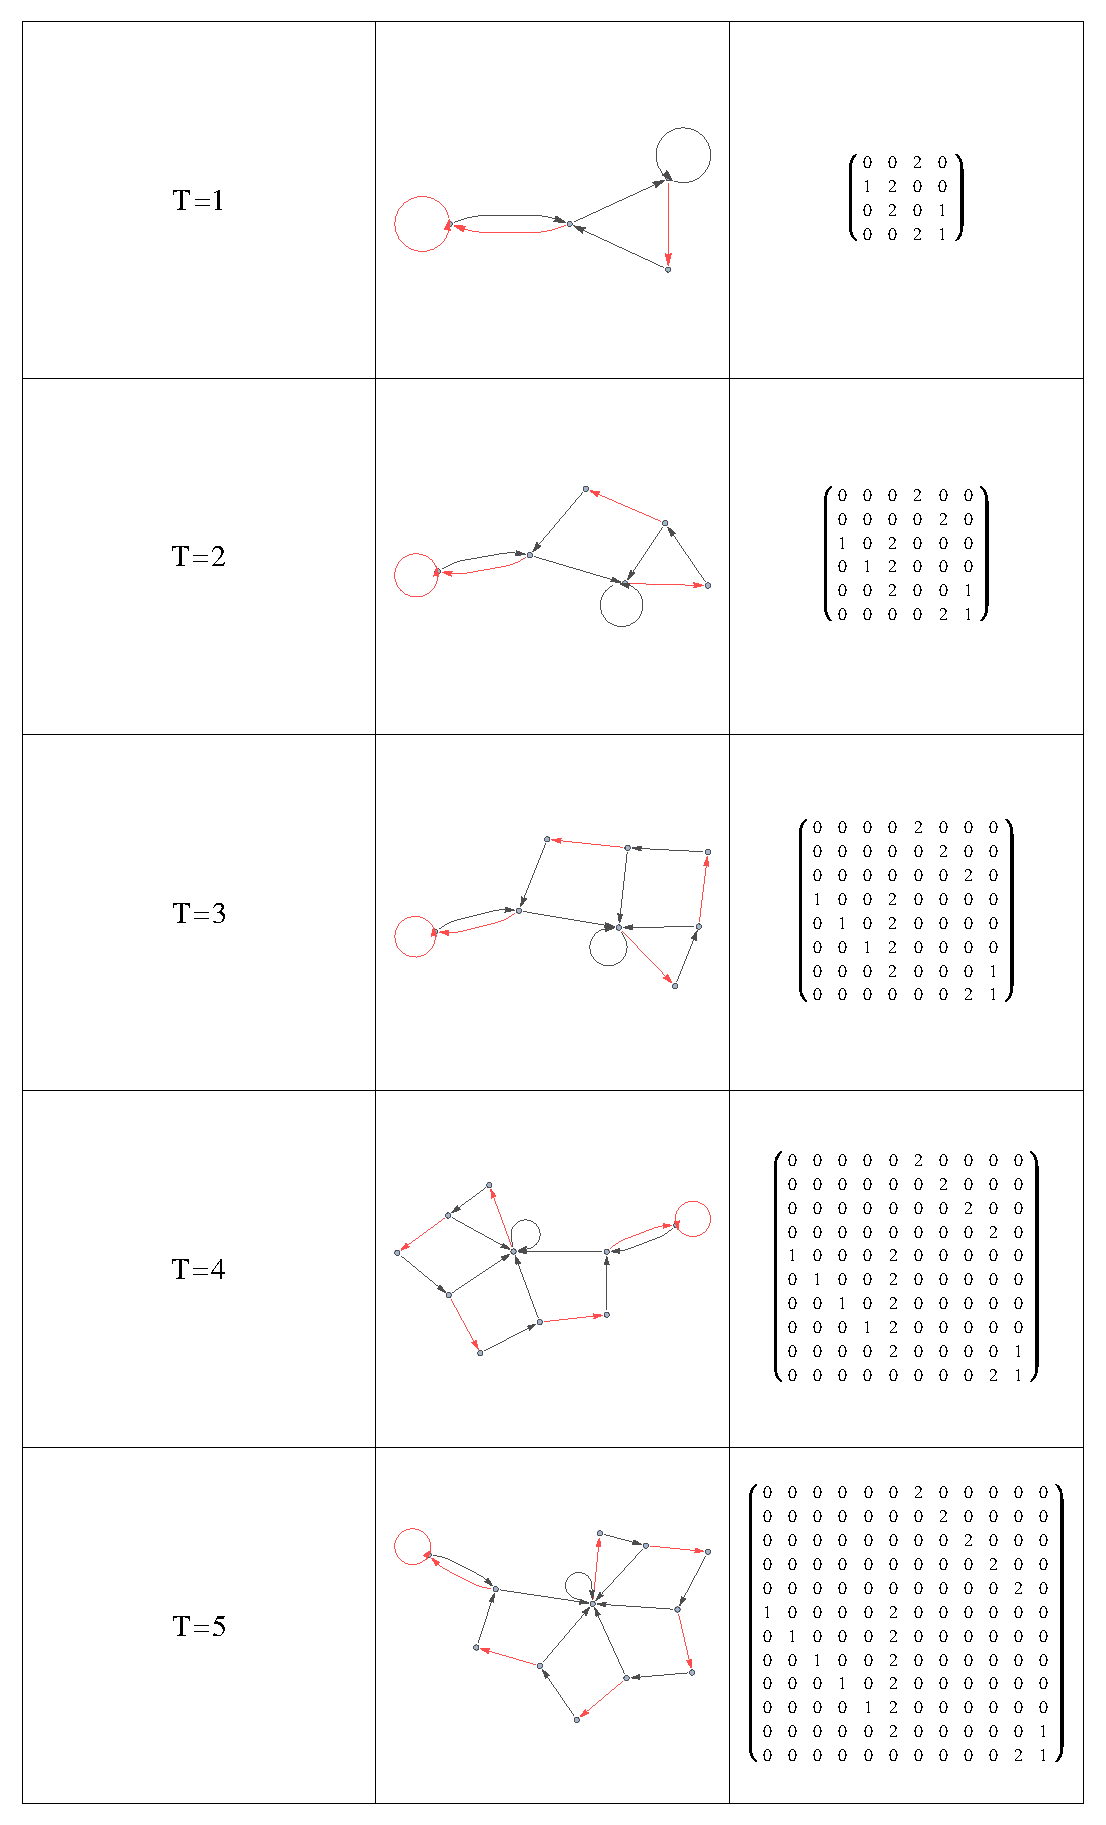
\includegraphics[scale=0.32]{img/mat/matr184.eps}
\caption{Regra 184.}
\label{tab:mr184}
\end{center}
\end{table}

\begin{table}[H]
\begin{center}
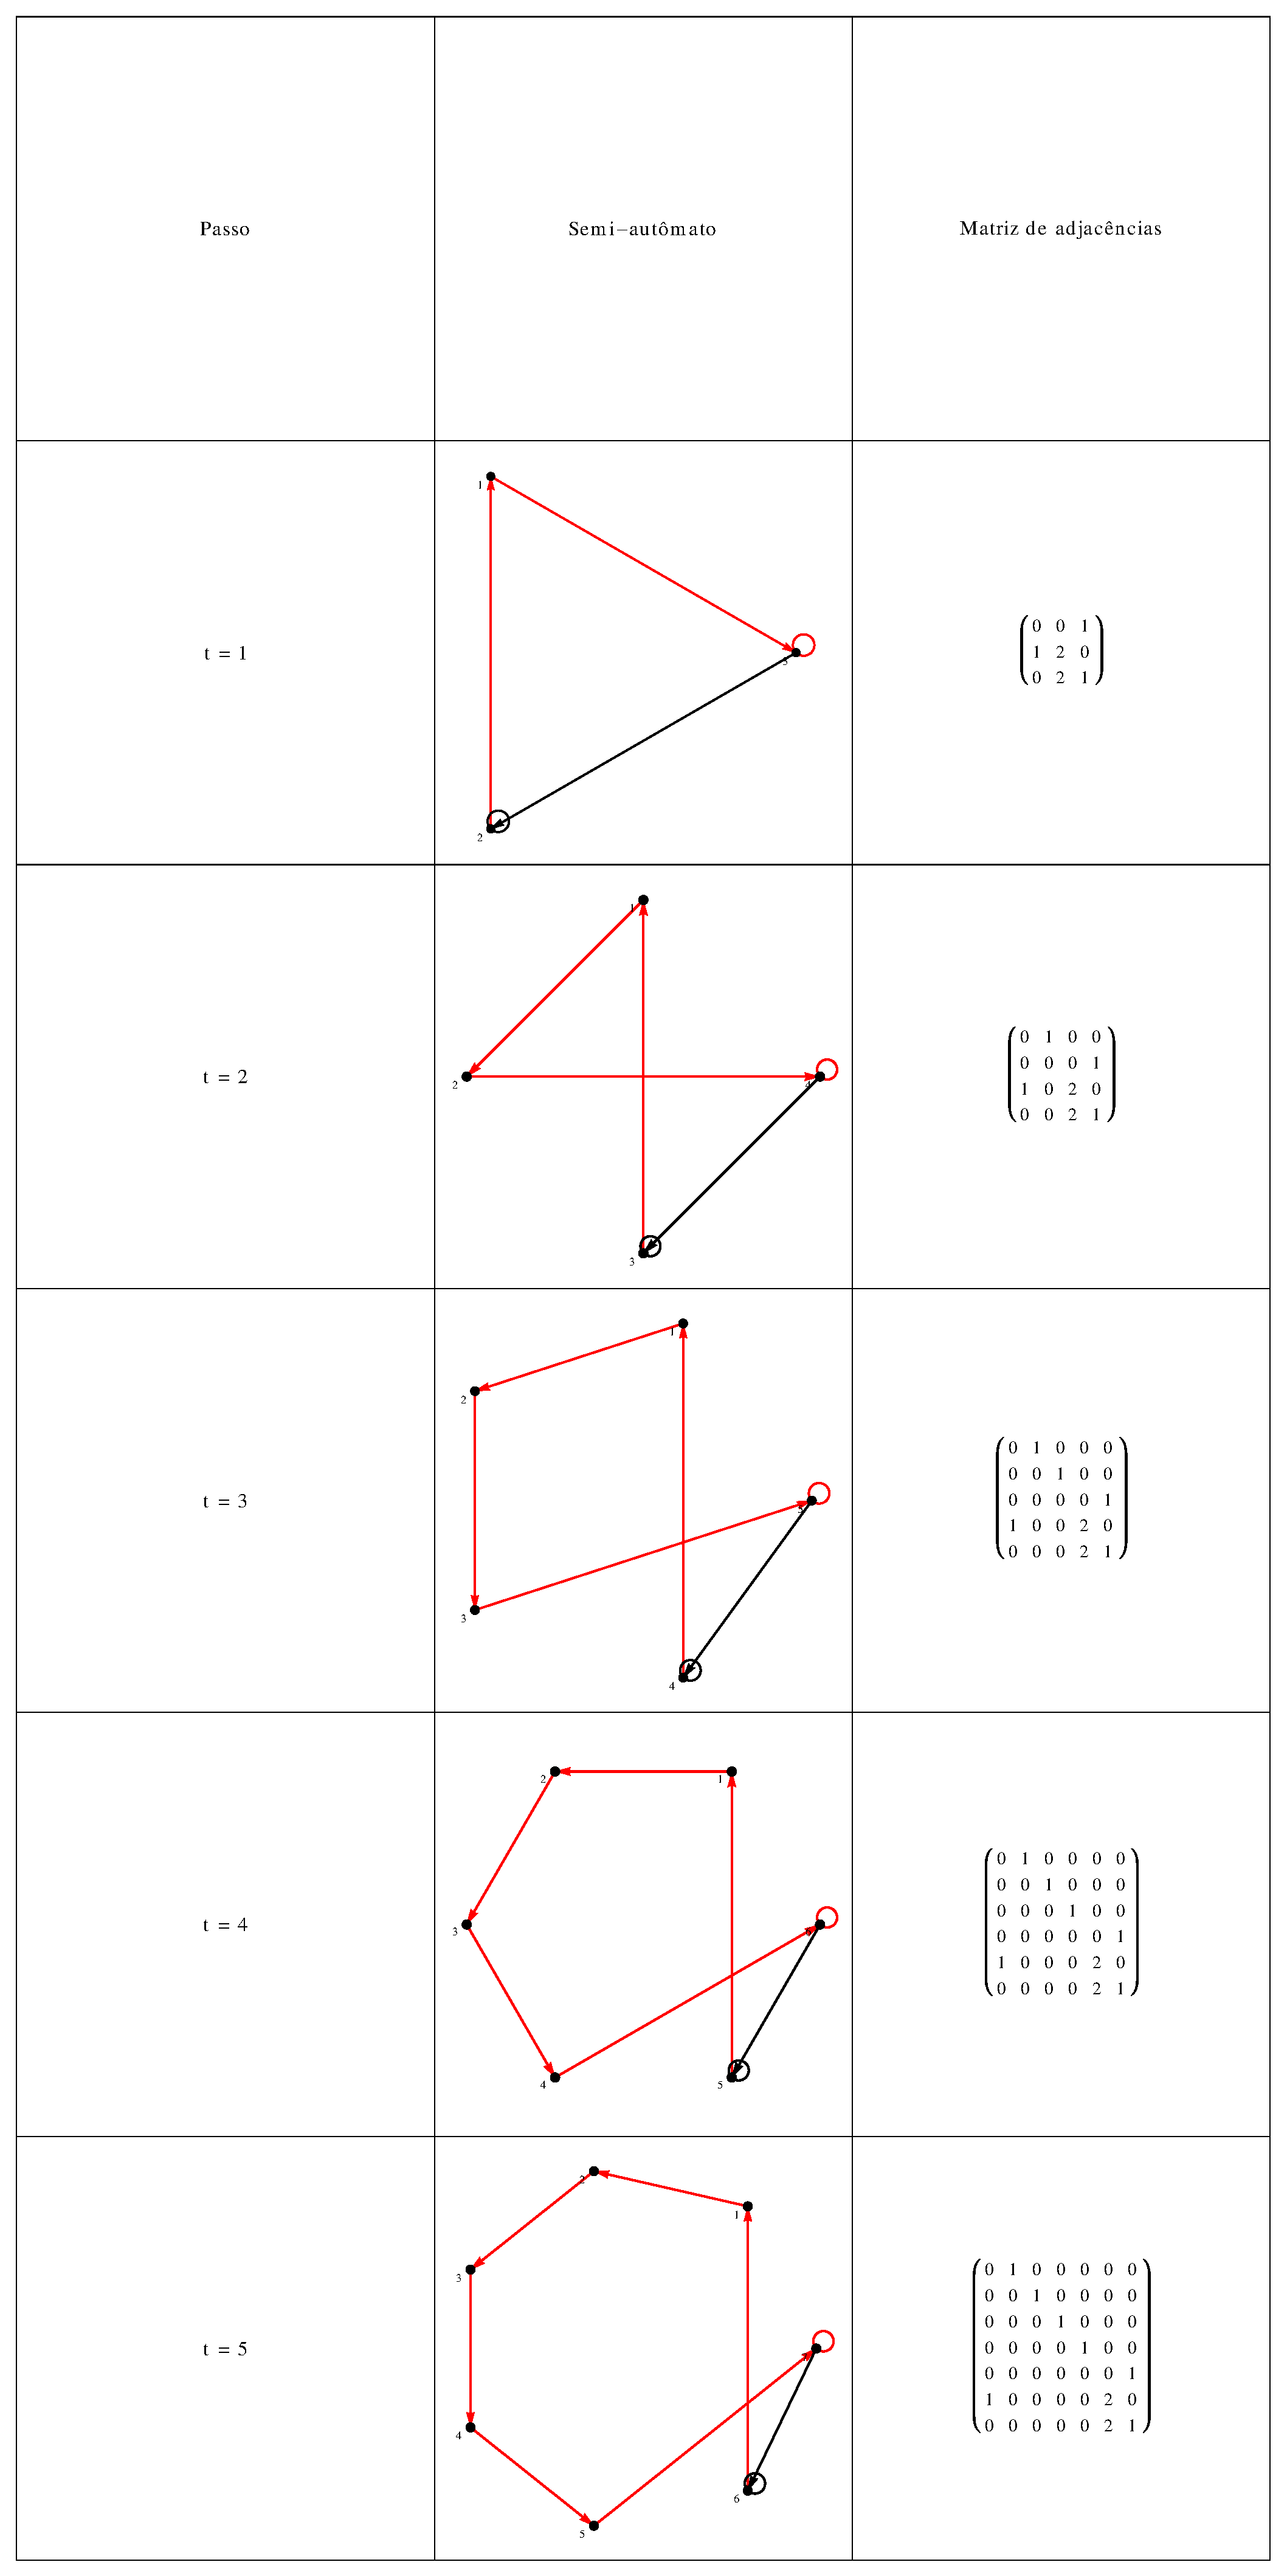
\includegraphics[scale=0.32]{img/mat/matr192.eps}
\caption{Regra 192.}
\label{tab:mr192}
\end{center}
\end{table}

\begin{table}[H]
\begin{center}
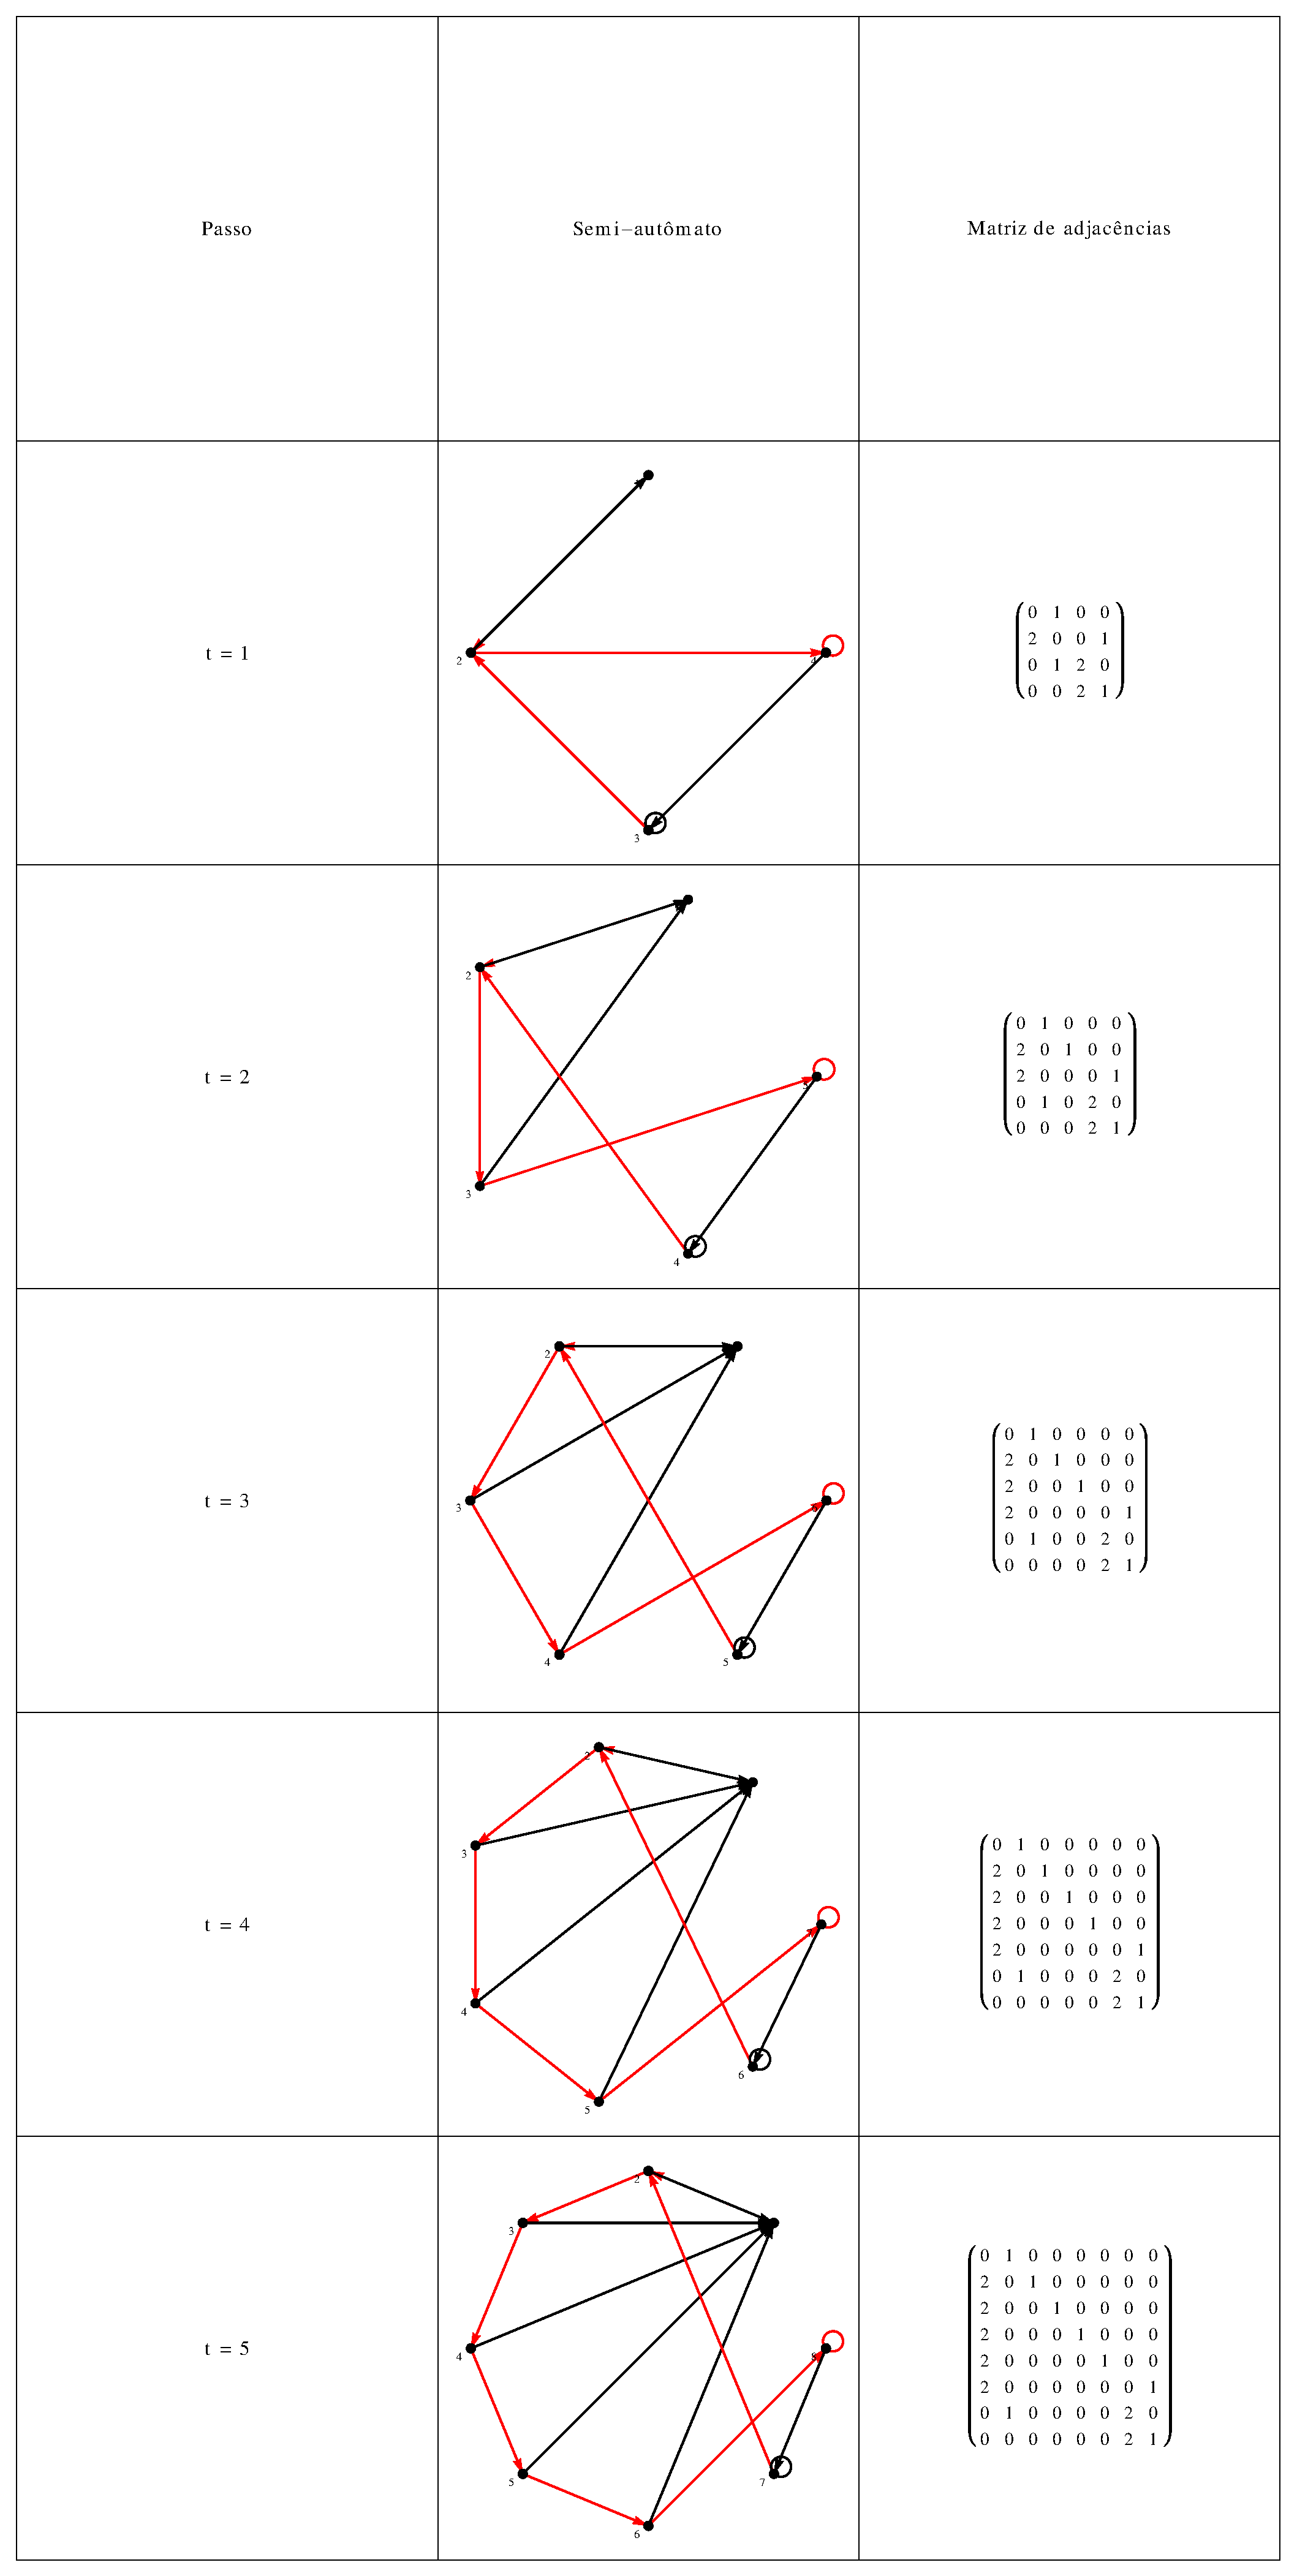
\includegraphics[scale=0.32]{img/mat/matr196.eps}
\caption{Regra 196.}
\label{tab:mr196}
\end{center}
\end{table}

\begin{table}[H]
\begin{center}
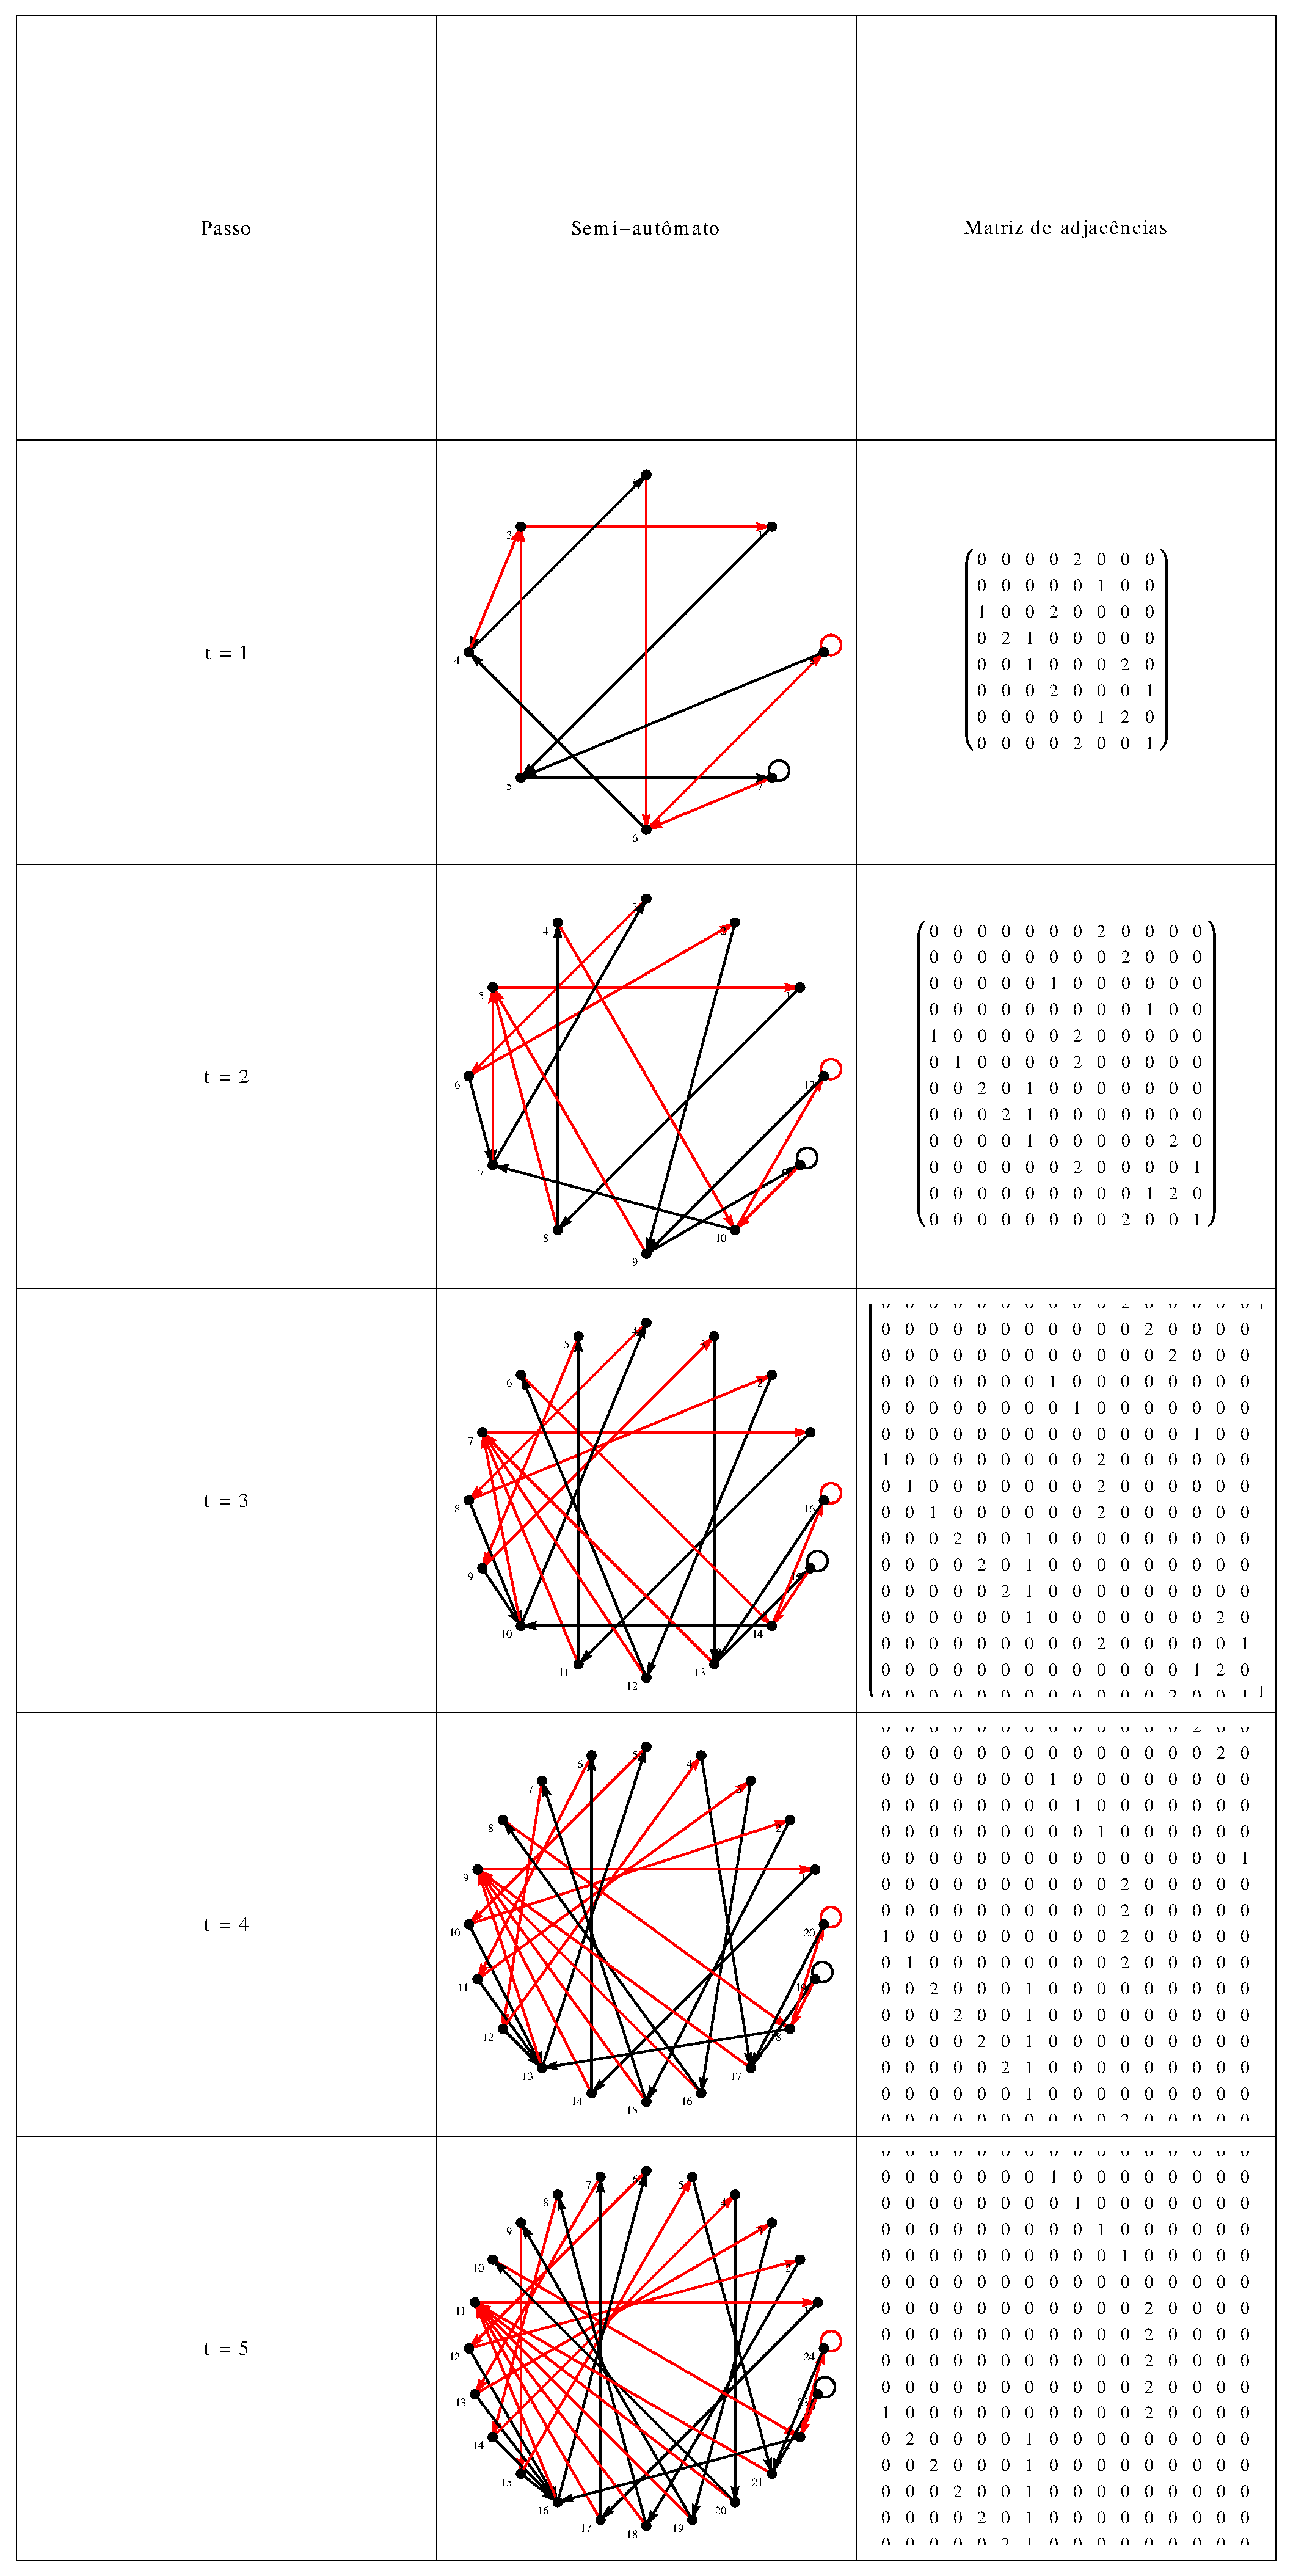
\includegraphics[scale=0.32]{img/mat/matr212.eps}
\caption{Regra 212.}
\label{tab:mr212}
\end{center}
\end{table}

\begin{table}[H]
\begin{center}
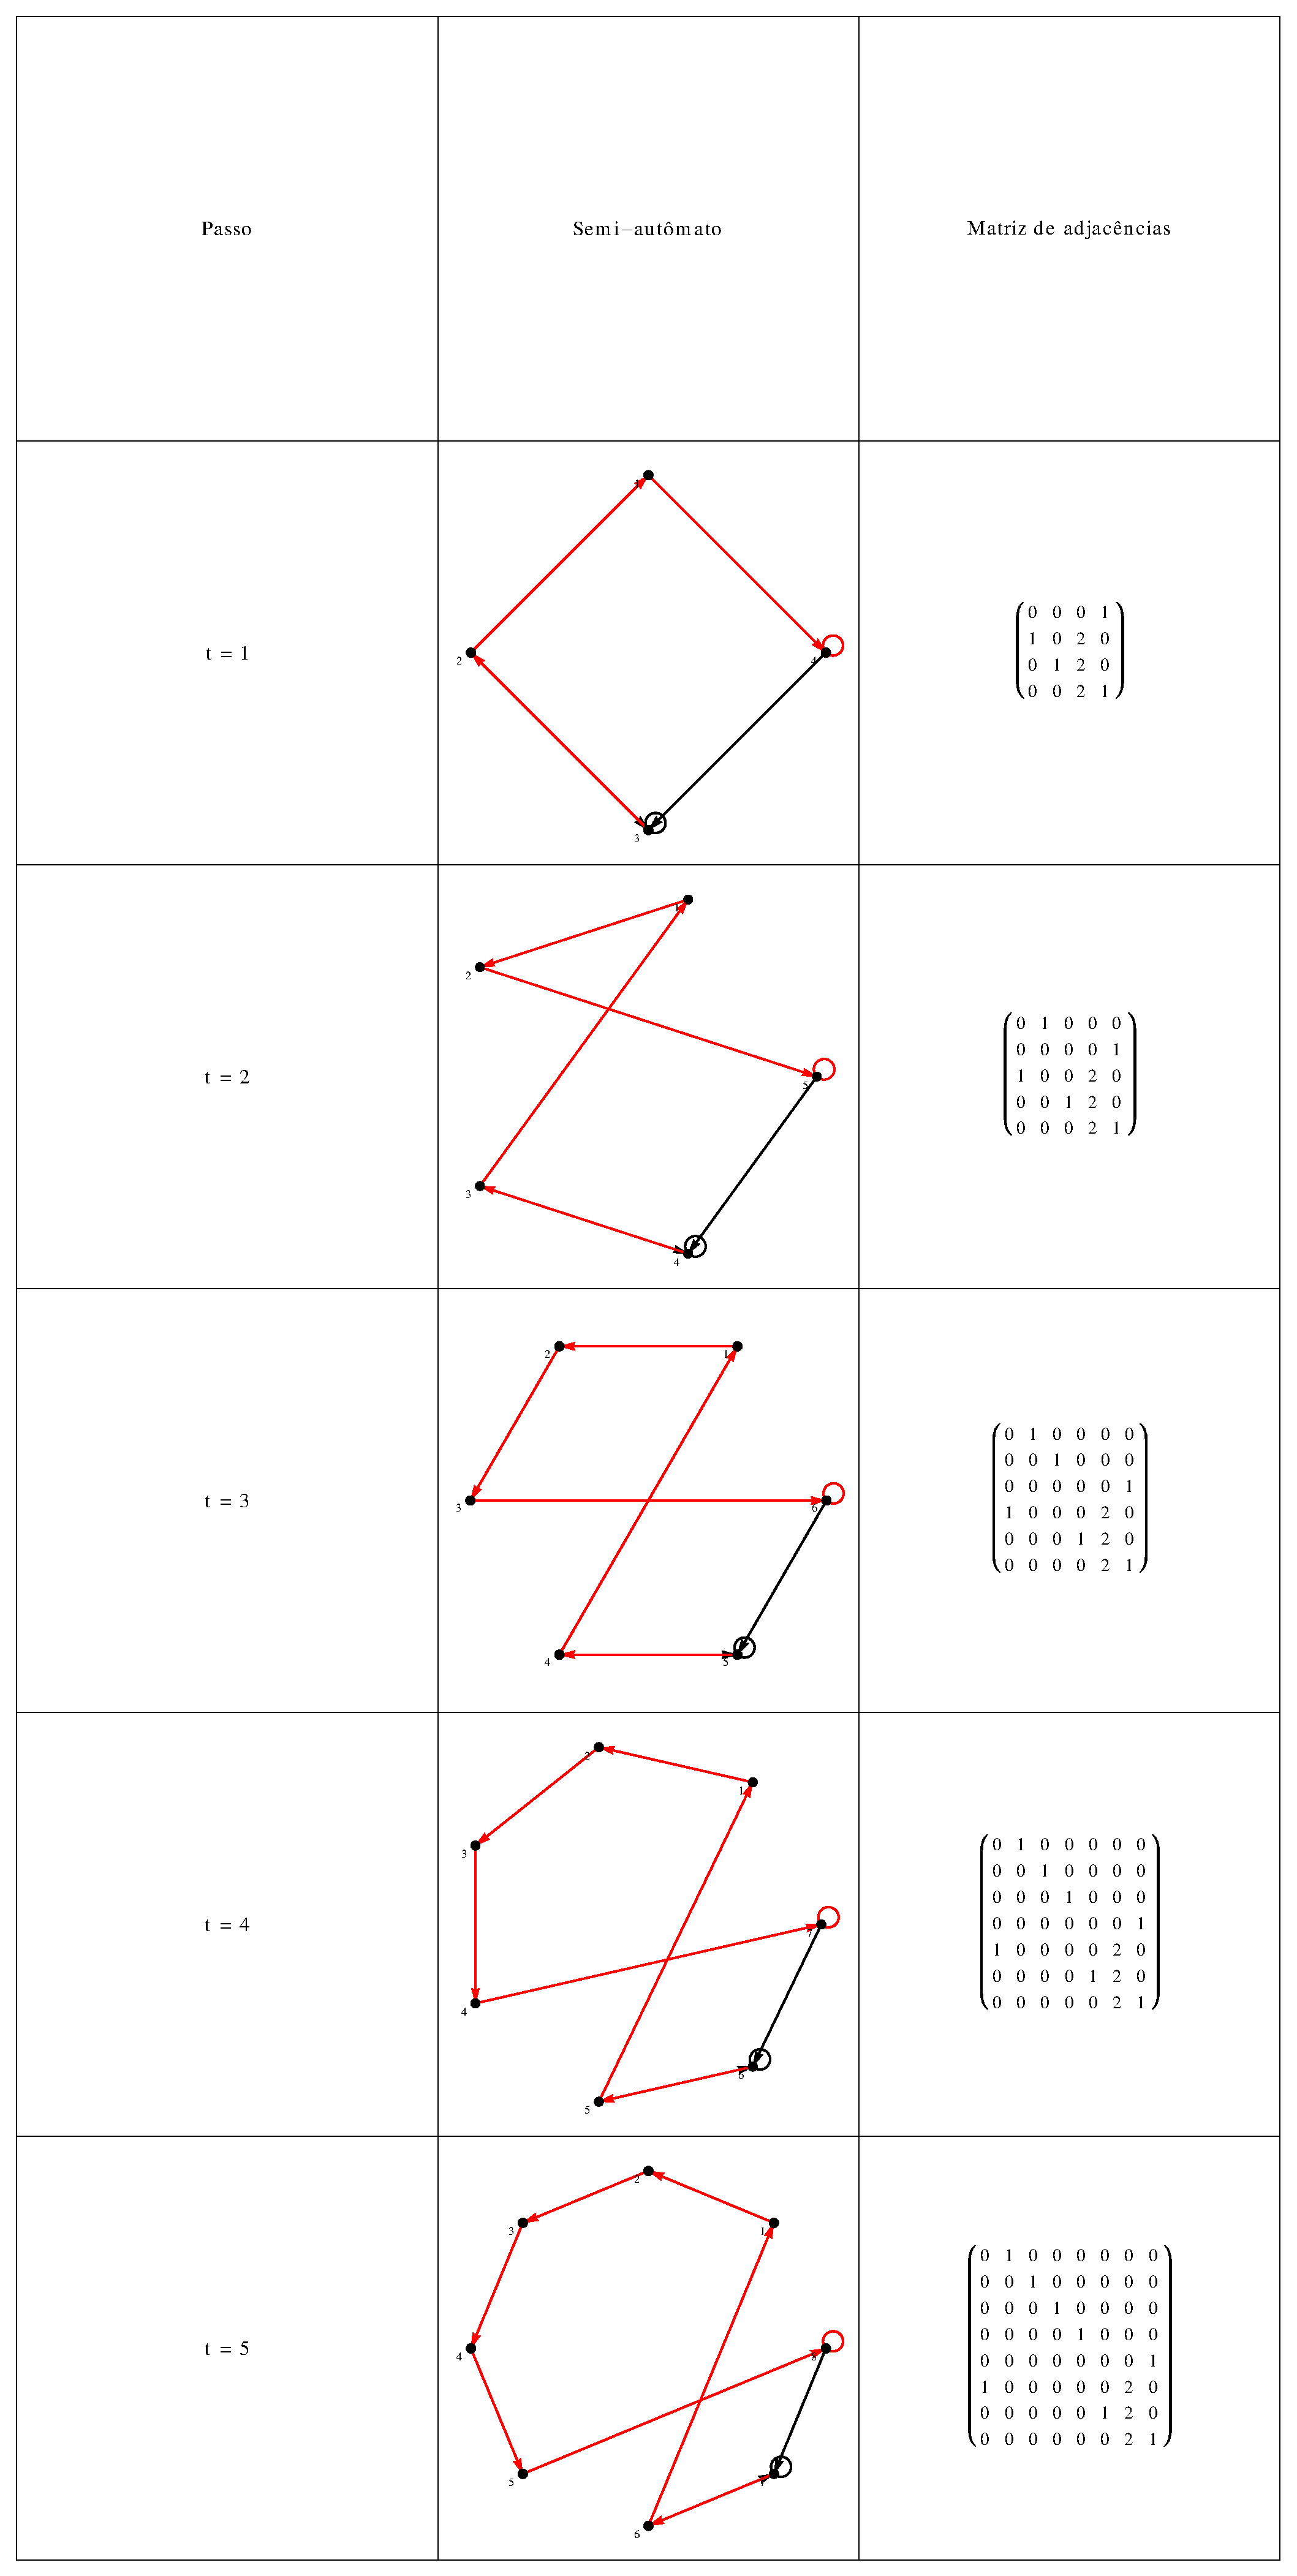
\includegraphics[scale=0.32]{img/mat/matr224.eps}
\caption{Regra 224.}
\label{tab:mr224}
\end{center}
\end{table}

\begin{table}[H]
\begin{center}
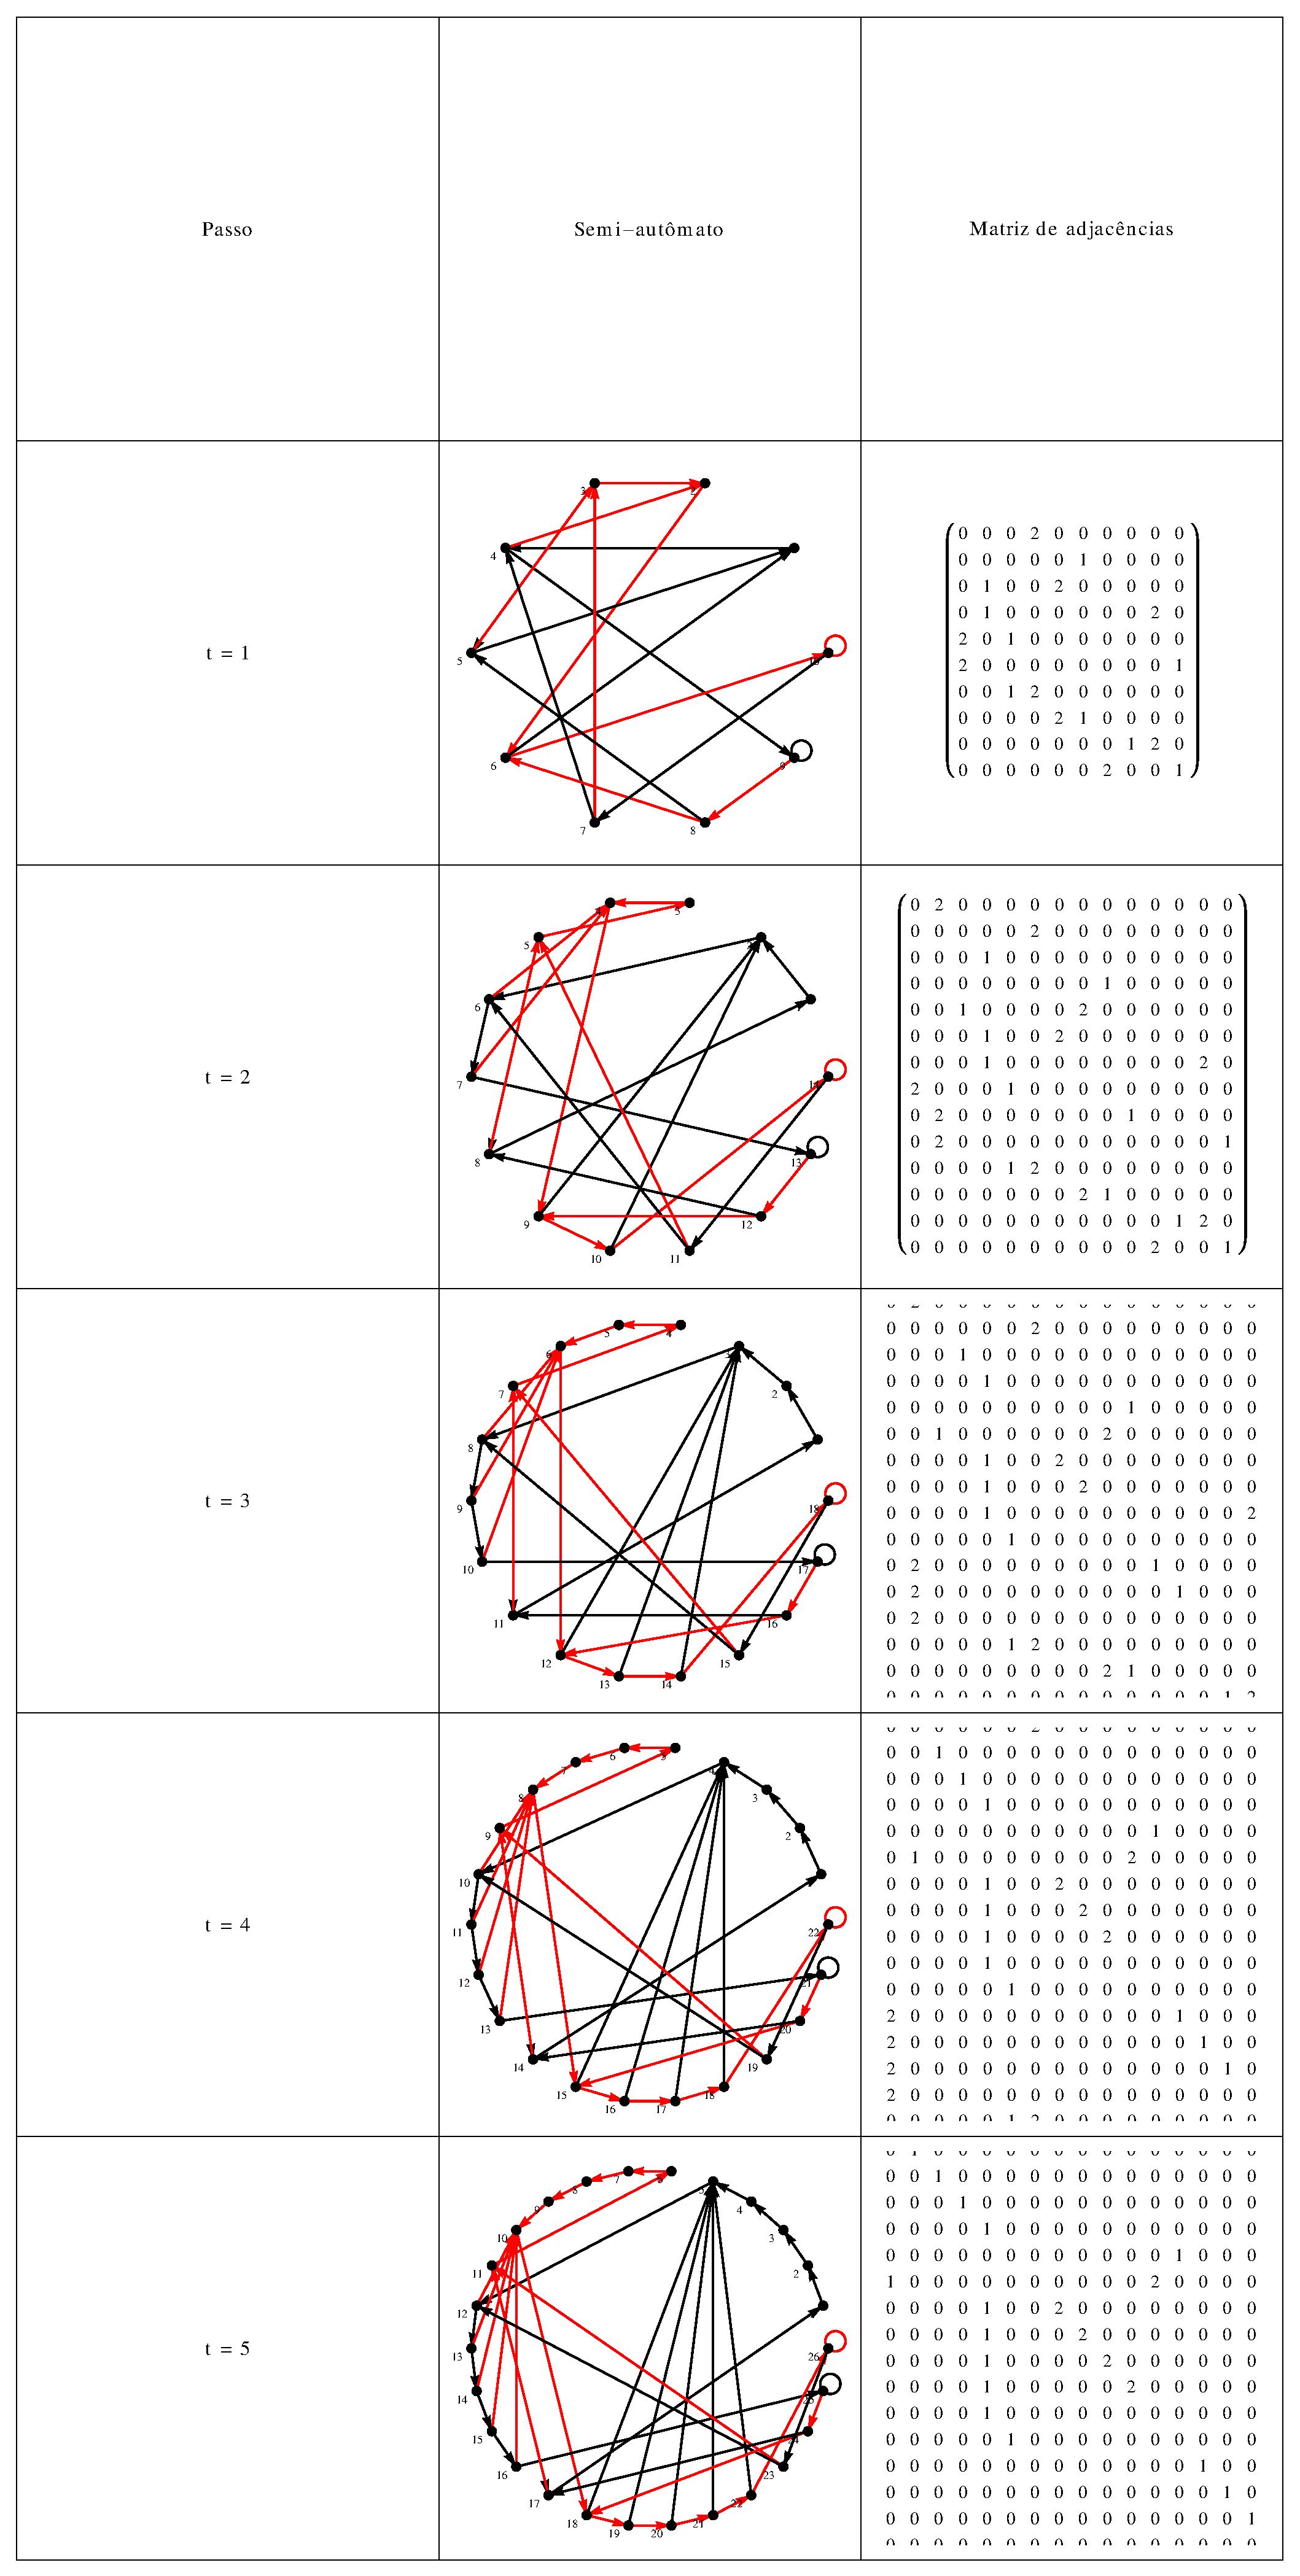
\includegraphics[scale=0.32]{img/mat/matr232.eps}
\caption{Regra 232.}
\label{tab:mr232}
\end{center}
\end{table}

\def\refname{Referências Bibliográficas}
\bibliography{masterthesis}
\addcontentsline{toc}{section}{Referências Bibliográficas} 
\bibliographystyle{abnt-alf}

\end{document}

% vim:set spell spelllang=pt
